\documentclass[apj]{emulateapj}
\usepackage{times}
%\newcommand{\mdot}{M$_{\odot}$\,}
\usepackage{natbib}

\usepackage[backref,breaklinks,colorlinks,citecolor=cyan]{hyperref} 
%\setlength{\parindent}{0pt}
\usepackage{booktabs}
\usepackage{graphicx}
\usepackage{bm}
%\usepackage{deluxetable}
\usepackage{multirow}
\usepackage{enumitem}
\usepackage{amsmath}

\shorttitle{Cosmic evolution of the \mbh-host relation}
\shortauthors{X. Ding et al.}

\begin{document}

\def\lcdm{$\Lambda$CDM}
\def\hst{{\it HST}}
\def\efr{$R_{\mathrm{eff}}$}
\def\galfit{{\sc Galfit}}
\def\mbh{$\mathcal M_{\rm BH}$}
\def\lhost{$L_{\rm host}$}
\def\jcap{Journal of Cosmology and Astroparticle Physics}
\def\halpha{${\it H}\alpha$}
\def\hbeta{${\it H}\beta$}
\def\sersic{S\'ersic}
\def\lenstronomy{{\sc Lenstronomy}}
\def\Reff{{$R_{\mathrm{eff}}$}}
\def\kms{km~s$^{\rm -1}$}
\def\sigstar{{$\sigma_*$}}
\def\smass{{$M_*$}}
\newcommand{\Mgii}{Mg$_{\rm II}$}
\newcommand{\Civ}{C$_{\rm IV}$}

\title{The mass relations between supermassive black holes and their host galaxies at $1< z<2$ with \hst-WFC3}

\author{Xuheng Ding\altaffilmark{1, 2}, John Silverman\altaffilmark{3}, Tommaso Treu\altaffilmark{1}, Andreas Schulze\altaffilmark{6}, Malte Schramm\altaffilmark{6}, Simon Birrer\altaffilmark{1},  Knud Jahnke, Federica Duras\altaffilmark{4, 5}, Angela Bongiorno\altaffilmark{5}, et al.
 }
 \email{dxh@astro.ucla.edu}
\altaffiltext{1}{Department of Physics and Astronomy, University of California, Los Angeles, CA, 90095-1547, USA}
\altaffiltext{2}{School of Physics and Technology, Wuhan University, Wuhan 430072, China}
\altaffiltext{3}{Kavli Institute for the Physics and Mathematics of the Universe, The University of Tokyo, Kashiwa, Japan 277-8583 (Kavli IPMU, WPI)}
\altaffiltext{4}{Dipartimento di Matematica e Fisica, Universit� Roma Tre, via della Vasca Navale 84, I-00146, Roma, Italy}
\altaffiltext{5}{INAF Osservatorio Astronomico di Roma, via Frascati 33, 00040 Monteporzio Catone, Italy}
\altaffiltext{6}{National Astronomical Observatory of Japan, Mitaka, Tokyo 181-8588, Japan}

\begin{abstract}

The tight correlations between the mass of a supermassive black hole (\mbh) and its host galaxy properties suggests an evolutionary connection. A powerful way to test this co-evolution hypothesis is to trace the correlations back in cosmic time. For this purpose, we obtained multi-band {\it Hubble Space Telescope} of  a sample of 32 X-ray-selected broad-line (type-1) AGN at $1.2<z<1.7$ (look-back time 8-10 Gyrs). By applying state-of-the art tools to the images we obtained accurate host galaxy luminosity and stellar mass. The black hole mass (\mbh) is based on published near-infrared spectroscopic observations of the broad \halpha~and \hbeta~emission lines, which avoids potential unknown systematic uncertainties associated with the less well calibrated UV lines \Civ\ or \Mgii, commonly used at these redshifts. We compare the \mbh-\lhost~and \mbh-\smass~relations to those of local active galaxies, accounting for selection effects, to infer their evolution. The \mbh-\lhost relation is inconsistent with the local one, accounting for passive evolution, indicating that the BHs at higher redshift resides in less luminous galaxies than today. The \mbh-\smass\ of our high redshift sample is consistent with the local \mbh-\smass$_{\rm bluge}$ relations. Considering that our sample are composed of bulge and disk components, we are forced to concluded that our results consistent to a scenario that the growth of the black hole predates that of the bulge.
\end{abstract}

\keywords{galaxies: active --- galaxies: evolution}

\section{Introduction}
\label{sec:introduction}
%\citep[e.g.,][]{Park15,Kormendy13}

Most galactic nuclei are thought to harbor a supermassive black hole (BH), whose mass (\mbh) is well known to be correlated with the host properties, such as \mbh-host luminosity (\lhost), \mbh-stellar mass (\smass) and \mbh-stellar velocity dispersion(\sigstar). These tight correlations indicate a connection between nuclear activity and galaxy formation and evolution \citep[e.g.,][]{Mag++98, F+M00, M+H03, Gul++09,Beifi2012, H+R04, Geb++01b, Gra++2011}.
Currently, the physical mechanism that can produce such a tight relationship is unknown, due to the daunting range of scales between the BHs dynamical sphere and their host galaxy. On the one hand, cosmological simulations of structure formation are able to reproduce the mean local correlations considering the active galactic nucleus (AGN) feedback as the physical driver \citep{Springel2005, Hopkins2008, Matteo2008, DeG++15}.
On the other hand, \citet{Peng2007, Jahnke2011, Hirschmann2010} show that, without the need of physical coupling, another possibility is a statistical convergence from the galaxy mergers which reproduces the observed correlations.

A powerful way to understand the origin of these correlations is to study them as a function of redshift, determining how and when they emerged and evolved over cosmic time \citep[e.g.,][]{TMB04,Sal++06,Woo++06, Jah++09,SS13}. During the past decade, there has been much progress on this front at $z<1$ using type 1 AGNs. For example, the work by \citet{Park15, Tre++07, Pen++06qsob} demonstrated that \mbh\ at fixed bulge luminosity compared to the local relations. This offset is consistent with a scenario in which supermassive BHs were built up first with galaxy then growing around their deep potential wells. Similarly, the works by \citet{Bennert11, Woo++08} agreed to this scenario by studying the \mbh-\smass and \mbh-\sigstar relations. Nevertheless, the evolution is detected at low significance given the considerable error bars, and some studies report results consistent with no evolution \citet{SS13, Sun2015, Cisternas2011}.

In order to make progress it is important to reduced as much as possible the uncertainties and take great care of selection effects and systematic errors. First, one needs to deal with the inherent uncertainties in BH mass estimates using the so-called "virial" method. In particular, many studies rely on \mbh\ estimates using the \Civ\ (or \Mgii) line that may have unknown systematics, such as non-virial component of the BLR gas, when compared to local samples with masses based on broad Balmer lines \citep[i.e. \halpha\ and \hbeta,][]{Schulze2018, Baskin2005, Trakhtenbrot2012}. Second, since the host information is swamped by the bright nuclear light, measuring the host galaxy properties is challenging. Great care is required for modeling the point spread function and whenever possible it is beneficial to study lensed quasars, since lensing magnifies the host image to lensed arcs \citep{Pen++06qsob, Ding2017a, Ding2017b}. Last but not least, the selection function needs to be taken into account when intepreting the observations \citep{Treu2007, Lauer2007}. For instance, it has been demonstrated \citep{Schulze2011, Schulze2014} that selecting bright AGNs at high redshift results in display steeper slopes than random ones, suggesting the selecting effects can exhibit faster evolution than a random sample. It is also important to consider the selection function when comparing the observed scaling relations with simulated ones \citep{DeG++15}.

In this study, we aim to make progress by making use of a large sample with high-quality data both for the measurement of both the host properties and the \mbh, extending to the highest redshifts where evolutionary effects should be strongest \citep{DeG++15}. In practice, we aim to determine whether AGNs have begun to couple to their host galaxy at $1.2<z<1.7$, an epoch when supermassive BH close to its peak accretion history \citep{Aird2015}.  In this redshift range, we measure 32 host galaxies properties using \hst\ imaging data, and estimate their \mbh\ based on the robust \halpha\ and \hbeta, using the multi-object spectrograph Subaru/FMOS. Our study overcomes the biases in the following way. First, to minimize selection bias, we select AGNs that fall below the knee of the black hole mass function. Second, we estimate \mbh\ using Balmer lines which avoids the systematics by \Mgii. Third, our X-ray selected sample have lower nuclear-to-host ratios which facilitate the galaxy mass measurements. Moreover, 21/32 systems in our sample have two-band \hst\ data (i.e. WFC3+ACS), whose multi-band information provides reliable K-correction and stellar mass inference. Given the high-quality data at such redshift, we can test whether the growth of BH predates that of the host by a factor of at least $1.7$ $(\sim0.23$ dex). 

The paper is organized as follows. We briefly describe the sample selection and the BH mass of the sample in Section~\ref{sec:data}. We describe the observation and collect the PSF library in Section~\ref{observation}. In Section~\ref{sec:analysis} we decompose our sample and study the host galaxy surface photometry. In Section~\ref{sec:result}, we use the multi-band host magnitudes to infer their stellar population, which we applied to derive the rest-frame R band \lhost\ and \smass and compared to the local samples. Discussion and conclusion are presented in Section~\ref{sec:dis} and Section~\ref{sec:sum}. 

Throughout this paper, we adopt a standard concordance cosmology with $H_0= 70$ km s$^{-1}$ Mpc$^{-1}$, $\Omega{_m} = 0.30$, and $\Omega{_\Lambda} =
0.70$. Magnitudes are given in the AB system.

%\section{Observations and data reduction}
%\label{sec:data}
%In this section, we summarize the sample selection, observations, and data reduction of our sample. 

\section{Sample selection and \mbh}
\label{sec:data}
%How the samples are selection.\\
%Where are they from?
%\\The redshift range? In a table?

%We aim to study the relation between the BH masses (\mbh) and their host galaxy properties including luminosities (\lhost) and stellar mass (\smass) to redshift at $z>1$. For this propose, 



We focus on the broad-line (type-1) AGNs as provided by the X-ray coverage of COSMOS \citep{Civano2016}, (E)-CDFS-S \citep{Lehmer2005, Xue2011}, and SXDS \citep{Ueda2008} fields. We select the broad-line AGNs at redshift region $1.2<z<1.7$ which cover a BH range $7.5<{\rm log}$\mbh $<8.5$. The Near IR spectra of AGNs are available from the survey of Subaru's Fiber Multi-Object Spectrograph \citep[FMOS, ][]{Kimura2010, Schulze2018}, a near-infrared (0.9-1.8 $\mu m$) spectrograph have with 400 apertures. The FMOS survey provides the best \mbh\ estimates by \halpha\ and \hbeta\ lines out to $z\sim1.7$ \citep{Greene2005, Matsuoka2013, Nobuta2012}. Overall, our final sample is composed of 32 new observations by HST/WFC3. Table~\ref{tab:objlist} list all the AGN systems analyzed in this work.

The \mbh\ of type-1 AGNs can be inferred using the so-called virial method \citep{Peterson2004, Shen2013}. The kinematics of the broad-line region (BLR) trace the gravitational field of the central supermassive black hole, assuming the gravity dominates the motion of the BLR gas. In this scenario, the width of the emission-line provided the scale of the velocity, while the AGN continuum luminosity establish an empirical scale of the BLR size. As a result, the estimation of the \mbh\ is achieved by these measurements.

For our targets, the \halpha\ and \hbeta\ emission-line properties have been investigated by \citet{Schulze2018} using the multi-object spectrograph Subaru/FMOS. We referred to that paper for the details of continuum fitting and emission line modeling. Since the other compared AGNs in the literature used different calibrations of the virial method, we compare the difference among the recipes by \citet{Schulze2018, McG++08, Ding2017b} and adopt a list of consistent ones to cross-calibrate the \mbh\ for all the samples, in order to avoid any systematic bias in Section~\ref{mbh}.

\subsection{Comparison sample}
\textcolor{blue}{
We aim to collect the \mbh-\lhost\ and \mbh-\smass\ relations of our samples and comparing to the ones at different redshift. 
For calibrating with the local relation, we use the local AGN measurements by \citet{Ben++10} and \citet{Bennert++2011} (hereafter, B10 and B11a) to define our zero-point. The sample by B10 consistent 19 \mbh-\lhost\ relations with reliable \mbh\ measured using reverberation-mapped (uncertainty level $\sim0.15$ dex). The work of B11 contains 25 \mbh-\smass\ local active AGN analysis, where the \mbh\ are measured from the single-epoch method (\mbh\ uncertainty level $\sim0.4$ dex). To increase the local \smass\ and \mbh\ to the higher range, we also include the inactive galaxies (mainly ellipticals or S0) as done by \citet{H+R04}. It is worth note that in the local comparison sample, the bulge mass is equivalent to the total stellar mass for the local comparison sample. In other words, it is the local \mbh-\smass$_{Bulge}$ relation that we compared. }

\textcolor{blue}{
Including the compared samples at the intermediate redshift range would help to understand the redshift evolution of these correlations. We compared intermediate redshift AGNs for the \mbh-\lhost\ relation include 52 sample by \citet{Park15} at $0.36<z<0.57$ and 27 sample by \citet{Bennert11, SS13} at $0.5<z<1.9$. Moreover, \citet{SS13} also derive the \smass\ which enable us to compare to the \mbh-\smass\ relation at $0.5<z<1.2$. }


\subsection{BH masses}
\label{mbh}
 %Our selected systems are broad-line (type-1) AGNs whose \mbh\ can be estimated from single-epoch spectroscopy using the so-called virial method \textcolor{blue}{FMOS (e.g. McLure 2002; Shen 2013)}. This estimation is achieved by the assumption that the empirical scaling size of the BLR and the line-of-sight velocity width can be inferred in turn continuum luminosity ($L _{\lambda_{\rm line}}$) and emission line width (FWHM), respectively.
To avoid any systematic bias between our samples and the literature ones, we compared the recipes as introduced by \citet{Schulze2018, Ding2017b}. We find that the \hbeta\ estimator is very consistent ($<0.03$~dex) between the two references. Moreover, in \citet{Schulze2018}, the cross-calibrate between the \halpha\ and \hbeta\ are consistent. Thus, we adopt the virial formalism from \citet{Schulze2018}:

\begin{eqnarray}
\label{eq:Ha}
\log \left(\frac{\mathcal M_{\rm BH} (H\alpha)}{M_{\odot}}\right)&~=~& 6.71+0.48 \log \left(\frac{ \lambda \rm L _{H\alpha}}{10^{42}{\rm erg~s^{-1}}}\right) \nonumber\\
&~+~& 2.12 \log \left(\frac{\rm FWHM(H\alpha)}{1000 ~{\rm km~s^{-1}}}\right).
\end {eqnarray}

and

\begin{eqnarray}
\label{eq:Hb}
\log \left(\frac{\mathcal M_{\rm BH}(H\beta) }{M_{\odot}}\right)&~=~& 6.91+0.50\log \left(\frac{ \lambda \rm L _{\lambda_{5100}}}{10^{44}{\rm erg~s^{-1}}}\right) \nonumber\\
&~+~& 2.0 \log \left(\frac{\rm FWHM(5100)}{1000 ~{\rm km~s^{-1}}}\right) , 
\end {eqnarray}

Having defined the recipes, we estimate the \mbh\ by adopting the emission line properties measured by \citet{Schulze2018}. 14 of the overall systems have both \halpha\ and \hbeta\ emission line information; we adopt the averaged \mbh\ value. We summarized the inference of the \mbh\ together with the properties of the emission line in Table~\ref{tab:result_mbh}.

\section{\hst\ observations}
\label{observation}
%\subsubsection{HST image Observation}
% The AGN surface photometry in IR Channel Filters.\\
The high spatial resolution of the host image is required for the decomposition of the nuclear/host emission and the accurate estimate of the host stellar mass. All the new 32 AGN systems were observed with the HST/WFC3 infrared channel, as the HST program GO-15115, PI: John Silverman. We selected to use the filters F125W $(1.2<z<1.44)$ and F140W $(1.44<z<1.7)$ according to the redshift of the targets. This selection ensures that the broad \halpha\ line ($4000\AA$) is not present in the bandpass so as not to contaminate the host emissions due to the broad wings of the PSF.

%Drizzling, background noise...
For each of the 32 new AGNs we took six separate exposures with $\sim399s$ (i.e. total exposure time $\sim2394s$). Table~\ref{tab:objlist} lists the details of the observation. The six exposures for each dither image were combined with the {\sc astrodrizzle} software package, with an output pixel scale of 0\farcs{0642} by setting \texttt{pixfrac} parameter as 0.8 using the \texttt{gaussian} kernel. 
To accurately estimate the background light which could come from both the sky and the detector, we adopt the {\sc photutils} to measure the photometry.

Multi-band information provides the spectral energy distributions (SED) at a more precise level. 21/32 of our sample have rest-frame UV images by \citet{Scoville2007}. Images were taken through the wide ACS/F814W filter at four dither pointing with $507s$ exposures. The final image is drizzled to 0\farcs{03} pixel scale. Given the multi-band image for these systems, we are able to infer their host color and assess the contribution of both the young and old stellar population to the stellar mass budge \citet{Gallazzi2009} which insures an accurate inference of rest-frame R-band luminosity by K-correction, stellar mass and star formation rate (SFR). 

%\subsubsection{AGN Emission Line}
%\label{sec:bh_mass}
% The introduction of the BH inferred by the board emission line.

 
%\section{Analysis}
\subsection{PSF library}
\label{sec:psf_library}
%Introduce the PSF library
The knowledge of the PSF is crucial for the AGN imaging decomposition, especially when the nuclear image is unresolved with light distributed as the point source. The PSF is known to be vary across the detector and with time, due to the effect of aberrations and breathing. Simulated PSF, such as {\sc TinyTim} ones, are usually insufficient matches to observations for our purposes \citet{Mechtley2012}. Stars within the fields provide a better description than the simulated PSF, since they were observed simultaneously with the science targets and reduced and analyzed in the same way \citet{Kim2008, Park15}

To minimize the impact of the mismatch, we build a PSF library by selecting all the isolated, unsaturated PSF-stars with high S/N from our entire program. The selection consists of the following steps. We first adopt the identified stars as candidates from the COSMOS2015 catalog by \citet{Laigle2016}. A lot of bright stars with intensity similar to the AGNs were excluded by \citet{Laigle2016}; in the second step, we manually select the PSF-like objects as candidates. We then remove the non-ideal PSF candidates based on their intensity, FWHM, central symmetry and any that were contaminated by nearby objects. In the end, the PSF library contains 78 and 37 PSFs for F140W and F125W, respectively.

We assume that the stars in the library are representative of the possible PSFs in our program. Therefore, we assume that the PSF library gives a good representation of the dominant source of uncertainty as well as the best fit.
%In the next subsection, we carry out the AGN decomposition using each PSF. We rank their performance based on the goodness (i.e. $\chi^2$) so that the final inference of the host properties are weighted from the top-rank PSFs.



%\label{sec:analysis}

%\subsection{Surface Photometry}
%\subsubsection{PSF library}    
%\subsubsection{Surface Photometry modeling method}
\section{AGN-host Decomposition}
\label{sec:analysis}
%Introduce the lenstronomy. Model the PSF in each library.\\
%Inspired by Simon's work, we rank the performance of the each PSF and weight for the final fitting result. 
We simultaneously fit the two-dimensional flux distribution of the center nuclear and the underlying host galaxy. Following common practice, we assume the unresolved nuclear as a scaled point source, while the host galaxy as a \sersic\ profile. Note that the actual morphologies of the host galaxies could be more complicated (e.g. bulge+disk). However, the purpose of adopting the \sersic\ model is a simplified a first-order approximation of the surface brightness distribution with a flexible parameterization which provides sufficient freedom to infer the host flux, given the high redshift range of our sample. Furthermore, we fit other galaxies that happen to be close to the AGN as additional \sersic\ model, to account for any potential contamination. \textcolor{blue}{The systems CID206 and ECDFS-358 have nearby objects which could not be described by \sersic\ model, we thus mask these objects in the fitting.}

%Introduce Lenstronomy:
We adopt the imaging modeling tool \lenstronomy\ \citep{lenstronomy} to perform the decomposition of the host and nuclear light. \lenstronomy\ is a multi-purpose open-source gravitational lens image modeling python package. 
Its flexibility enables us to turn off the lensing channel and focus on the AGN decomposition\footnote{For a sanity check, we compared the performance of \lenstronomy\ to the most commonly used galaxy modeling software {\sc Galfit} and confirm that the consistent result could be obtained with the same fitting ingredients provided.}. The maim advantage over {\sc Galfit} is that \lenstronomy returns the full posterior of the parameter and not just the best fit model and the Laplace approximation of the uncertanties. The input ingredients to \lenstronomy\ include:
\begin{enumerate}
\item AGN imaging data. \\
-- Using aperture photometry, we find that an aperture size with radius $\sim1\farcs{}5$ covers sufficient AGN light our samples. By default, we cut out the AGN image to a $61\times61$ pixels box (i.e. $4''\times 4''$). If needed, the larger size box would be sufficient to include the nearby objects. 
\item Noise level map.\\
-- The origin of the noise in each pixel stems from the read noise, background noise and Poisson noise by the astronomical sources themselves. To take them into account, we measure the read noise and background noise level directly from the empty regions of the data. We calculate the effective exposure time of each pixel based on the drizzled \texttt{WHT} array maps to infer the Poisson noise level. 
\item PSF. \\
-- 
The PSF is directly taken from the PSF library. Usually, a mismatch exists when subtracting the AGN as the scaled PSF, especially at the central parts. While modeling multiply imaged AGN, this mismatch can be mitigated with PSF reconstruction by the iterative method \citep{Chen2016, Birrer2018}.  However, this approach requires multiple images which are not available in our case.  We remedy this deficiency by using a broad library which should contain sufficient information to cover all the possible PSF. 
\end{enumerate}

%Introduce the final inference using fitting:
The host properties of one AGN system is inferred via the following steps. First, we model the AGN and host using each PSFs in the library. Inputting the fitting ingredients to \lenstronomy, the posterior distribution of the parameter space is calculated and optimized by adopting the Particle Swarm Optimizer (PSO)\footnote{Note that, the \lenstronomy\ enables one to further infer the parametric confidence interval using MCMC. However, in our case, given a fixed PSF, the $1-\sigma$ inference of each parameter are extremely narrow.}.
To avoid any unphysical inferences, we set the upper and lower limit for the key parameters as effective radius \Reff$\in[0\farcs{}1,1\farcs{}]$, and Sersic index $n\in[1,7]$. Then, we rank the performance of each PSF based on the $\chi^2$ value and select the top-eight PSFs as representative of the best fit PSFs. We infer the host property (i.e., host flux, \Reff, Sersic index $n$) using a weighted arithmetic mean. The weight is calculated by:
\begin{eqnarray}
\label{eq:weights}
w_i = exp \big(- \alpha \frac{ (\chi_i ^2 - \chi_{best} ^2 )}{2 \chi_{best} ^2} \big),
\end{eqnarray} 
where the $\alpha$ is an inflation parameter so that when $i=8$:
\begin{eqnarray}
\label{eq:alpha}
\alpha \frac{ \chi_{i=8} ^2 - \chi_{best} ^2 }{2 \chi_{best} ^2} = 2,
\end{eqnarray} 
The goal of this recipe is to weight each PSF based on their relative goodness of fit, while ensuring at least eight are used to capture the range of systematic uncertainties. The answers would not change significantly if we had chosen a different number of PSFs, as we show below.

Note that since each AGN system was observed in different location of the detector and at a different time, the top-eight PSFs usually vary from one AGN system to another. Given the weights, the inferred value of host properties and the root-mean-square ($\sigma$) are calculated as:
\begin{eqnarray}
\label{eq:infer_value}
\bar{x}  =  \frac{  \sum_{i=1}^{8}   x_i * w_i  }{\Sigma w_i} ,
\end{eqnarray} 
\begin{eqnarray}
\sigma =   \sqrt{ \frac{  \sum_{i=1}^{8}   (x_i -  \bar{x} ) ^2 * w_i  }{\Sigma w_i} }.
\end{eqnarray} 

In Figure~\ref{fig:AGN_decomp}, we demonstrate the optimized results inferred by \lenstronomy, including the AGN images, best-fit models, image subtract point source (i.e. host) and the residuals. As an example, the weights adopted in the analysis of system COSMOS-CID1174 are listed in Table~\ref{tab:weight_CID1174}. In order to quickly overview our inference, we summarize the relations of the properties between effective radius \Reff, 2) \sersic\ index $n$ and 3) host to total flux ratio in Figure~\ref{fig:flux_r_n_corner}.

The inference of the host properties is weighted by eight top-ranked PSFs. For a smaller number of PSFs one tends to underestimate the uncertainties. To understand how the choice of the number of top-ranked PSF affects our inference, we compare to the one inferred by five and ten top-ranked PSFs. As shown in Figure~\ref{fig:hist_compare}, the results are very consistent, meaning that the host inference is solid when the amount of selected PSF exceeds five. 

%The inference of F814w data.
18/32 systems in the COSMOS field have ACS/F184W imaging data. We infer their host properties using the same approach used for the WFC3-IR data. The field of view by ACS are larger than WFC3, and we collected in total 174 ACS PSFs in the library. In principle, the host inference by IR band is superior to the one by UV band, giving that the effects of dust extinction and contrast between the (blue) AGN and (red) host. Thus, we fix the \Reff\ and \sersic\ $n$ as the value inferred by IR band, assuming that the morphology of the galaxy is consistent between ACS and WFC3.

We list all the inference of the host galaxy properties in the Table~\ref{tab:result_sersic}.

\section{Results}
\label{sec:result}

\subsection{Host galaxy properties}
We derive the rest-frame R band magnitude ($M_R$) and luminosity ($L_R$) of our sample based on their filter magnitude. 18/32 systems have multi-band host magnitude which ables us to select the best stellar population that could fit the overall sample. We find that the 1~Gyr stellar population with solar metallicity by Chabrier initial mass function (IMF) \citep{Bruzual2003} could well match the color between the WFC3 and ACS band magnitude of these samples. Adopting the color information, we perform the K-correction and derive the rest-frame R band magnitude of our sample. Given that the WFC3 filter we selected is very close to the rest-frame R band, we expect the $M_R$ uncertainty level raised by this K-correction is within 0.05~mag. We derive the rest-frame R band luminosity by $\log L_R/L_{R, \odot} = 0.4 (M_{R, \odot}-M_R)$, where $M_{R, \odot}=4.61$ \citep{Blanton07}.

Taking the stellar population, we estimate the stellar mass content of each host galaxy according to the mass-to-light ratio of the stellar population we adopted. The raised uncertainty level to the stellar mass is expected to be within 0.1~dex.

%\textcolor{red}{Need to add the uncertainty level of their inference}.

The inferred $L_R$ and $M_*$ are listed in Table~\ref{tab:result_sersic}. In the rest of this section, we compare their relations to to the \mbh.

\subsection{\mbh-\lhost\ relation}
We show our measurements of the \mbh-\lhost\ relation together with the comparison sample in Figure~\ref{fig:ML}, panel (a). Following common practice, we fit the local relation as a linear relation,
\begin{eqnarray}
\label{eq:MLlocal}
\log \big( \frac{\mathcal M_{\rm BH}}{10^{7}M_{\odot}})= \alpha + \beta \log(\frac{L_R}{10^{10}L_{\odot}}),
\end {eqnarray}
which enables direct comparison to the distant sample. The figure shows that the observed \mbh-\lhost\ relation for our measurements is nearly identical to the local and intermediate ones, indicating that the black hole mass and the host luminosity located at a similar relation at different galaxy age. However, considering that both the black hole and host galaxy are expected to evolve over cosmic time, it is essential to transfer high-$z$ measurements to their values at today so as to compare them in an equivalent frame. Especially, in a passive evolution scenario, we expect \lhost\ to fade over time. 

We follow \citet{Ding2017b} and parametrize the luminosity evolution with the functional form as
$d{\rm mag}_{\rm R} \sim d\log(1+z)$, i.e.,
\begin{eqnarray}
\label{eq:L_relation}
\log(L_{R,0})=\log(L_{R}) - 1.48 \log (1+z).
\end{eqnarray} 
This formalism is more accurate to fit a broad range redshift comparing to a single slope as $d$mag$/dz$. We refer to \citet[][section 5.4]{Ding2017b} for more details. Transferring the \lhost\ to today, we show the evolution-corrected \mbh-\lhost\ relation in Figure~\ref{fig:ML}, panel (b) and find that, at fixed \mbh, the BH in the more distant universe tends to reside in less luminous hosts.

To quantitatively understand this trend, we fit the offset as a function of redshift in form as:
\begin{eqnarray}
\label{eq:offset}
\Delta \log \mathcal M_{\rm BH}= \gamma \log (1 + z),
\end{eqnarray} 
where $\Delta \log \mathcal M_{\rm BH} = \log \big( \frac{\mathcal M_{\rm  BH}}{10^{7}M_{\odot}}) -\alpha-\beta\log(\frac{L_{R,0}}{10^{10}L_{\odot}})$. The best-fit and  1-$\sigma$ inference are $\gamma = 0.69 \pm 0.15$.

Given that the current result does not take into account selection effects yet, we will draw the conclusion in section~\ref{select_eff}.

\subsection{\mbh-\smass\ relation}
Analyzing the correlation of the \mbh-\smass\ would be more efficient to help directly understand the connection between their coevolution. In Figure~\ref{fig:MM}, we plot the \mbh-\smass\ relation and compare to the local and intermediate sample. We visually see that the mass distributions for the three samples are very similar. Similarly, we consider the local as linear relation to fit offset (i.e., $\Delta\log \mathcal M_{\rm BH}$) as a function of $\gamma \log (1 + z)$. We obtain the $\gamma  = 0.49 \pm 0.19$ which slightly indicates as the positive, see Figure~\ref{fig:MM-vz}, panel (a). We also show the ratio of \mbh-\smass of the three samples at different redshift in Figure~\ref{fig:MM-vz}, panel (b). We highlight that our results are less biased in both the measurement of \mbh\ and \smass. 

We highlight that the local sample employed are bulge-dominated galaxies and the adopted \smass\ are equivalent to their bulge masses. That is, we are comparing the \mbh-\smass$_{,total}$ at the distant universe to the \mbh-\smass$_{,bulge}$ at the local. Considering that a major part of the distant systems has indicated the disk component (i.e., the systems with fitted \sersic\ index close to 1), the \smass$_{,bluge}$ of them are supposed to be even less.

Without taking into account the selection effect, the direct comparison shows that the growth of the black hole predates that of the host bulge.

\subsection{Selection effect}
\label{select_eff}
\textcolor{red}{To be written after Daeseong's analysis.}.

\section{discussion}
\label{sec:dis}
\subsection{Systematic error}


In our analysis, we adopt one stellar population to the overall sample. We note that adopting the private stellar populations for these samples which have both multi-band host magnitude could be more robust in principle. However, considering that the host magnitude in ACS band is faint (host-total flux ratio $< 30\%$), the fidelity of the SED fitting is actually lost. Perhaps the best way to derive the stellar population is to combining our measurements to the ground-based photometry. \textcolor{red}{Describe the ground-based data}. In this paper, we focus on the decomposing of the AGN and carry out a rapid analysis of the \mbh-host relations. The measurements incorporating the ground-based photometry and the comparison with the simulations are presented in our companion paper.

\subsection{Comparison to the inactive galaxies}
We compared the morphology of AGNs host galaxies to the inactive galaxies in CANDLES imaging survey. We select 4401 inactive galaxies in a comparable redshift range ($1.2<z<1.7$) whose \sersic\ properties are inferred by \citet{VDwel++2012} by \galfit, and their stellar masses are derived by 3-D-HST spectroscopic survey \citep{Momcheva2016, Brammer2012}.

In Figure~\ref{fig:Mstar-rn}, we plot the \smass\ versus the \Reff\ and \sersic\ index. The color coding is based on the filter flux ratio between WFC3 and ACS. The distribution of \smass-\Reff\ relation show that our AGN hosts concentrate at the high end of the stellar mass, close to the red sequence. 

We also compare the histogram of the inferred \Reff\ and \sersic\ n to the inactive galaxies in Figure~\ref{fig:hist_rn}, where there is no significant difference between their distribution and median value. We perform the Kolmogorov?Smirnov test to interpret the p-value as 0.42 and 0.04 for \Reff\ and $n$, respectively.

%high
%The distribution shows that our AGN host are located at a higher end of the stellar mass at region where 

\subsection{JWST}

\section{Summary}
\label{sec:sum}
%We presented the study of the \mbh\ and host property's evolution to high redshift until 1.7.


\section*{Acknowledgments}
Based in part on observations made with the NASA/ESA Hubble Space Telescope, obtained at the Space Telescope Science Institute, which is operated by the Association of Universities for Research in Astronomy, Inc., under NASA contract NAS 5-26555. These observations are associated with programs
\#15115.

The authors fully appreciate the discussions with Vardha N. Bennert, Takahiro Morishita.

SB, TT and AJS acknowledge support by the Packard Foundation through a Packard Research fellowship to TT.

This work has made use of lenstronomy \citep{lenstronomy}, Astropy \citep{Astropy}, photutils, TOPCAT \citep{TOPCAT}, Matplotlib \citep{Matplotlib} and standard Python libraries.

\bibliographystyle{apj.bst}
\bibliography{references}

\begin{deluxetable}{llccccc}
\tablecolumns{7}
\tablewidth{0pt}
\tablecaption{Details of Observation} 
\tablehead{ 
\colhead{Object ID} &
\colhead{$z$} & 
\colhead{WFC3/Filter} &
\colhead{$RA$}&
\colhead{$DEC$}&
\colhead{Observing date}&
\colhead{Expousre time (s)}
\\ 
\colhead{(1)} &
\colhead{(2)} &
\colhead{(3)} &
\colhead{(4)} &
\colhead{(5)} &
\colhead{(6)} &
\colhead{(7)}
} 
\startdata
%\multicolumn{5}{c}{Sample presented in \citet{Treu+07}}\\
%\\
COSMOS-CID1174 & 1.552 & F140W & 150.2789 & 1.9595 & 2017-10-26 & 2395.4\\
COSMOS-CID1281 & 1.445 & F140W & 150.4160 & 2.5258 & 2018-11-26 & 2395.4\\
COSMOS-CID206 & 1.483 & F140W & 149.8371 & 2.0088 & 2017-10-23 & 2395.4\\
COSMOS-CID216 & 1.567 & F140W & 149.7918 & 1.8729 & 2017-10-23 & 2395.4\\
COSMOS-CID237 & 1.618 & F140W & 149.9916 & 1.7243 & 2018-06-03 & 2395.4\\
COSMOS-CID255$^a$ & 1.664 & F140W & 150.1017 & 1.8483 & 2019-03-16 & 2395.4\\
COSMOS-CID3242 & 1.532 & F140W & 149.7113 & 2.1452 & 2017-10-26 & 2395.4\\
COSMOS-CID3570 & 1.244 & F125W & 149.6411 & 2.1076 & 2017-10-27 & 2395.4\\
COSMOS-CID452 & 1.407 & F125W & 150.0045 & 2.2371 & 2017-10-25 & 2395.4\\
COSMOS-CID454 & 1.478 & F140W & 149.8681 & 2.3307 & 2018-02-26 & 2395.4\\
COSMOS-CID50 & 1.239 & F125W & 150.2080 & 2.0833 & 2017-10-23 & 2395.4\\
COSMOS-CID543 & 1.301 & F125W & 150.4519 & 2.1448 & 2018-04-30 & 2395.4\\
COSMOS-CID597 & 1.272 & F125W & 150.5262 & 2.2449 & 2018-11-25 & 2395.4\\
COSMOS-CID607 & 1.294 & F125W & 150.6097 & 2.3231 & 2017-10-25 & 2395.4\\
COSMOS-CID70 & 1.667 & F140W & 150.4051 & 2.2701 & 2017-10-27 & 2395.4\\
COSMOS-LID1273 & 1.617 & F140W & 150.0565 & 1.6275 & 2017-10-31 & 2395.4\\
COSMOS-LID1538 & 1.527 & F140W & 150.6215 & 2.1588 & 2018-05-01 & 2395.4\\
COSMOS-LID360 & 1.579 & F140W & 150.1251 & 2.8617 & 2017-10-30 & 2395.4\\
COSMOS-XID2138 & 1.551 & F140W & 149.7036 & 2.5781 & 2017-11-01 & 2395.4\\
COSMOS-XID2202 & 1.516 & F140W & 150.6530 & 1.9969 & 2017-11-05 & 2395.4\\
COSMOS-XID2396 & 1.600 & F140W & 149.4779 & 2.6425 & 2017-11-12& 2395.4\\
CDFS-1 & 1.630 & F140W & 52.8990 & -27.8600 & 2018-04-03 & 2395.4\\
CDFS-229 & 1.326 & F125W & 53.0680 & -27.6580 & 2018-04-04 & 2395.4\\ 
CDFS-321 & 1.570 & F140W & 53.0486 & -27.6239 & 2018-08-18& 2395.4\\ 
CDFS-724 & 1.337 & F125W & 53.2870 & -27.6940 & 2018-04-05 & 2395.4\\ 
ECDFS-358 & 1.626 & F140W & 53.0850 & -28.0370 & 2018-02-09& 2395.4\\ 
SXDS-X1136 & 1.325 & F125W & 34.8925 & -5.1498 & 2018-01-29& 2395.4\\ 
SXDS-X50 & 1.411 & F125W & 34.0267 & -5.0602 & 2018-03-01& 2395.4\\ 
SXDS-X717 & 1.276 & F125W & 34.5400 & -5.0334 & 2018-07-02 & 2395.4\\ 
SXDS-X735 & 1.447 & F140W & 34.5581 & -4.8781 & 2017-11-14 & 2395.4\\ 
SXDS-X763 & 1.412 & F125W & 34.5849 & -4.7864 & 2018-07-03 & 2395.4\\ 
SXDS-X969 & 1.585 & F140W & 34.7594 & -5.4291 & 2018-07-02 & 2395.4\\ 
\enddata
\label{tab:objlist}
\tablecomments{
Column 1: Object field and ID.
Column 2: Redshifts.
Column 3: WFC3 filter. Note that the targets from the COSMOS field also have ACS/F814W imaging.
Column 4 and 5: J2000 $RA$ and $DEC$ coordinates.
Column 6: The observing start date.
\\
$^a$For CID255, 3/6 of the dither WFC3 images are corrupted. We analyze this sample by a same approach, taking the 3 avalible frames.
}
\end{deluxetable}

\begin{deluxetable*}{ccccccc}
\tablecolumns{7}
\tablewidth{0pt}
\tablecaption{The host inference of CID1174} 
\tablehead{ 
\colhead{PSF rank} &
\colhead{total $\chi ^2$} & 
\colhead{weights $w_i$} &
\colhead{host flux (counts)} &
\colhead{host flux ratio}&
\colhead{\Reff (arcsec)}&
\colhead{\sersic\ $n$}
 \\ 
\colhead{(1)} &
\colhead{(2)} &
\colhead{(3)} &
\colhead{(4)} &
\colhead{(5)} &
\colhead{(6)} &
\colhead{(7)} 
} 
\startdata
%\multicolumn{5}{c}{Sample presented in \citet{Treu+07}}\\
%\\
1 & $8584.429$ & $1.000$ & $82.2$ & $35\%$ & $0\farcs{}345$ & $1.1$ \\
2 & $8646.711$ & $0.920$ & $99.1$ & $42\%$ & $0\farcs{}298$ & $1.9$ \\
3 & $8816.947$ & $0.734$ & $76.7$ & $33\%$ & $0\farcs{}365$ & $1.1$ \\
4 & $9304.841$ & $0.383$ & $128.6$ & $55\%$ & $0\farcs{}231$ & $2.8$ \\
5 & $9652.575$ & $0.241$ & $187.5$ & $79\%$ & $0\farcs{}116$ & $6.2$ \\
6 & $9917.101$ & $0.170$ & $100.2$ & $42\%$ & $0\farcs{}287$ & $2.1$ \\
7 & $10018.324$ & $0.148$ & $75.1$ & $32\%$ & $0\farcs{}365$ & $1.2$ \\
8 & $10087.456$ & $0.135$ & $79.8$ & $34\%$ & $0\farcs{}358$ & $1.2$ \\
\hline\\
Weighted value & & & $97.322\pm28.336$ & $42\%\pm12\%$& $0\farcs{}309\pm0\farcs{}065$  & $1.9\pm1.3$  \\
\enddata
\label{tab:weight_CID1174}
\tablecomments{
Column~1: Rank of the PSF from the library.
Column~2: Total $\chi ^2$ for the corresponding PSF.
Column~3: Weights for the inference.
Column~4-7: Fitted value for the host flux, host/total flux ratio, effective radius, and \sersic\ index.
For this sample, the inflation parameter $\alpha$ calculated by Eq.~\ref{eq:alpha} is 16.671.
}
\end{deluxetable*}

\tabcolsep=0.03cm
\begin{deluxetable*}
{@{\extracolsep{4pt}}lcccccccccc}   % need for the gap between the clines.
\tablecolumns{9}
\tablewidth{0pt}
\tablecaption{Inferred host galaxy properties for the 32 systems.} 
\tablehead
{ 
\colhead{Target ID}&
  \multicolumn{5}{c}{WFC3}&
  \multicolumn{3}{c}{ACS/F814W} &
   \multicolumn{2}{c}{host properties} \\
  \cline{2-6}  \cline{7-9} \cline{10-11}  \\
\colhead{}& 
\colhead{reduced $\chi ^2$}& \colhead{host-total flux ratio}& 
\colhead{\Reff}& \colhead{\sersic\ $n$}& 
\colhead{magnitude}&
\colhead{reduced $\chi ^2$}& \colhead{host-total flux ratio}& \colhead{magnitude} &
\colhead{$\log L_R$} &\colhead{$\log M_*$} \\
\colhead{}& 
\colhead{}& \colhead{}& 
\colhead{($\arcsec$)}& \colhead{}& 
\colhead{(AB system)}& \colhead{}& 
\colhead{}& \colhead{(AB system)} &\colhead{($L_{\odot,R}$)} & \colhead{(M$_{\odot}$)}\\
\colhead{(1)}& 
\colhead{(2)}& \colhead{(3)}& 
\colhead{(4)}& \colhead{(5)}& 
\colhead{(6)}& \colhead{(7)}& 
\colhead{(8)}& \colhead{(9)}&
\colhead{(10)}& \colhead{(11)}
}
\setlength{\tabcolsep}{20pt}
\renewcommand{\arraystretch}{1.5}
\startdata 
CID1174 & $2.307$ & $42\%\pm12\%$ & $0\farcs{}31\pm0\farcs{}07$ & $1.9\pm1.3$ & $21.48\substack{+0.37\\-0.28}$ & $2.496$ & $11\%\pm1\%$ & $23.21\substack{+0.11\\-0.10}$ & $11.13\substack{+0.15\\-0.11}$ &$10.85\substack{+0.18\\-0.15}$\\[3pt]
CID1281 & $1.322$ & $49\%\pm14\%$ & $0\farcs{}24\pm0\farcs{}09$ & $3.2\pm1.5$ & $22.88\substack{+0.36\\-0.27}$ & $1.378$ & $19\%\pm8\%$ & $24.83\substack{+0.60\\-0.38}$ & $10.49\substack{+0.15\\-0.11}$ &$10.21\substack{+0.18\\-0.15}$\\[3pt]
CID206 & $2.054$ & $35\%\pm24\%$ & $0\farcs{}29\pm0\farcs{}15$ & $3.1\pm2.5$ & $21.82\substack{+1.30\\-0.58}$ & $1.903$ & $8\%\pm2\%$ & $23.67\substack{+0.40\\-0.29}$ & $10.95\substack{+0.52\\-0.23}$ &$10.66\substack{+0.53\\-0.25}$\\[3pt]
CID216 & $1.514$ & $94\%\pm5\%$ & $0\farcs{}25\pm0\farcs{}06$ & $6.2\pm1.2$ & $21.51\substack{+0.05\\-0.05}$ & $1.425$ & $35\%\pm2\%$ & $23.45\substack{+0.05\\-0.05}$ & $11.13\substack{+0.03\\-0.03}$ &$10.85\substack{+0.10\\-0.10}$\\[3pt]
CID237 & $2.349$ & $30\%\pm6\%$ & $0\farcs{}87\pm0\farcs{}17$ & $4.7\pm1.7$ & $21.28\substack{+0.26\\-0.21}$ & $2.354$ & $3\%\pm2\%$ & $23.72\substack{+1.04\\-0.52}$ & $11.26\substack{+0.11\\-0.09}$ &$10.98\substack{+0.14\\-0.13}$\\[3pt]
CID255 & $1.625$ & $19\%\pm5\%$ & $0\farcs{}19\pm0\farcs{}06$ & $4.2\pm1.5$ & $21.61\substack{+0.37\\-0.28}$ & 2.858 & $4\%\pm2\%$ & $22.89\substack{+0.60\\-0.39} $& $11.17\substack{+0.15\\-0.11}$ &$10.89\substack{+0.18\\-0.15}$\\[3pt]
CID3242 & $2.751$ & $46\%\pm13\%$ & $0\farcs{}20\pm0\farcs{}16$ & $6.1\pm1.9$ & $21.16\substack{+0.35\\-0.26}$ & $2.596$ & $5\%\pm1\%$ & $23.60\substack{+0.34\\-0.26}$ & $11.25\substack{+0.14\\-0.11}$ &$10.97\substack{+0.17\\-0.15}$\\[3pt]
CID3570 & $1.665$ & $77\%\pm2\%$ & $0\farcs{}70\pm0\farcs{}01$ & $0.7\pm0.1$ & $21.16\substack{+0.02\\-0.02}$ & $1.332$ & $86\%\pm2\%$ & $22.97\substack{+0.01\\-0.01}$ & $11.07\substack{+0.02\\-0.02}$ &$10.79\substack{+0.10\\-0.10}$\\[3pt]
CID452 & $1.684$ & $75\%\pm4\%$ & $0\farcs{}37\pm0\farcs{}02$ & $1.4\pm0.2$ & $21.18\substack{+0.06\\-0.06}$ & $1.452$ & $38\%\pm1\%$ & $22.73\substack{+0.02\\-0.02}$ & $11.21\substack{+0.03\\-0.03}$ &$10.93\substack{+0.10\\-0.10}$\\[3pt]
CID454 & $2.203$ & $36\%\pm3\%$ & $0\farcs{}39\pm0\farcs{}02$ & $0.6\pm0.1$ & $21.20\substack{+0.08\\-0.07}$ & $1.291$ & $9\%\pm1\%$ & $23.35\substack{+0.06\\-0.06}$ & $11.19\substack{+0.04\\-0.04}$ &$10.91\substack{+0.10\\-0.10}$\\[3pt]
CID50 & $5.576$ & $17\%\pm9\%$ & $0\farcs{}16\pm0\farcs{}11$ & $3.2\pm2.2$ & $20.93\substack{+0.86\\-0.48}$ & $4.940$ & $5\%\pm3\%$ & $22.50\substack{+1.15\\-0.55}$ & $11.15\substack{+0.35\\-0.19}$ &$10.87\substack{+0.36\\-0.21}$\\[3pt]
CID543 & $1.902$ & $31\%\pm10\%$ & $0\farcs{}10\pm0\farcs{}00$ & $0.5\pm0.3$ & $21.99\substack{+0.41\\-0.30}$ & $1.435$ & $5\%\pm2\%$ & $23.77\substack{+0.53\\-0.36}$ & $10.79\substack{+0.16\\-0.12}$ &$10.51\substack{+0.19\\-0.15}$\\[3pt]
CID597 & $1.565$ & $42\%\pm17\%$ & $0\farcs{}17\pm0\farcs{}06$ & $1.8\pm0.8$ & $21.87\substack{+0.54\\-0.36}$ & $1.254$ & $12\%\pm1\%$ & $23.56\substack{+0.13\\-0.11}$ & $10.81\substack{+0.22\\-0.15}$ &$10.53\substack{+0.24\\-0.18}$\\[3pt]
CID607 & $1.692$ & $44\%\pm18\%$ & $0\farcs{}21\pm0\farcs{}09$ & $3.4\pm1.1$ & $21.19\substack{+0.58\\-0.37}$ & $2.590$ & $5\%\pm2\%$ & $23.57\substack{+0.51\\-0.35}$ & $11.10\substack{+0.23\\-0.15}$ &$10.82\substack{+0.25\\-0.18}$\\[3pt]
CID70 & $2.041$ & $20\%\pm5\%$ & $0\farcs{}42\pm0\farcs{}10$ & $3.6\pm1.0$ & $21.86\substack{+0.30\\-0.24}$ & $2.361$ & $2\%\pm1\%$ & $24.63\substack{+0.68\\-0.41}$ & $11.07\substack{+0.12\\-0.10}$ &$10.79\substack{+0.16\\-0.14}$\\[3pt]
LID1273 & $1.697$ & $53\%\pm9\%$ & $0\farcs{}30\pm0\farcs{}04$ & $1.2\pm0.5$ & $20.94\substack{+0.21\\-0.18}$ & $2.137$ & $6\%\pm1\%$ & $23.29\substack{+0.15\\-0.13}$ & $11.40\substack{+0.09\\-0.07}$ &$11.12\substack{+0.13\\-0.12}$\\[3pt]
LID1538 & $2.362$ & $44\%\pm8\%$ & $0\farcs{}18\pm0\farcs{}04$ & $2.8\pm0.5$ & $21.25\substack{+0.22\\-0.18}$ & $2.173$ & $8\%\pm1\%$ & $23.09\substack{+0.19\\-0.16}$ & $11.21\substack{+0.09\\-0.08}$ &$10.93\substack{+0.13\\-0.12}$\\[3pt]
LID360 & $3.918$ & $18\%\pm2\%$ & $0\farcs{}63\pm0\farcs{}02$ & $0.8\pm0.4$ & $21.46\substack{+0.14\\-0.12}$ & $4.914$ & $4\%\pm1\%$ & $23.25\substack{+0.17\\-0.15}$ & $11.17\substack{+0.06\\-0.05}$ &$10.88\substack{+0.11\\-0.11}$\\[3pt]
XID2138 & $1.597$ & $39\%\pm6\%$ & $0\farcs{}50\pm0\farcs{}03$ & $1.2\pm0.4$ & $21.87\substack{+0.17\\-0.15}$ & $2.731$ & $5\%\pm1\%$ & $23.90\substack{+0.31\\-0.24}$ & $10.98\substack{+0.07\\-0.06}$ &$10.70\substack{+0.12\\-0.12}$\\[3pt]
XID2202 & $3.23$ & $33\%\pm8\%$ & $0\farcs{}10\pm0\farcs{}00$ & $4.0\pm1.0$ & $21.16\substack{+0.30\\-0.24}$ & $3.852$ & $8\%\pm2\%$ & $22.59\substack{+0.29\\-0.23}$ & $11.24\substack{+0.12\\-0.10}$ &$10.96\substack{+0.16\\-0.14}$\\[3pt]
XID2396 & $3.669$ & $24\%\pm11\%$ & $0\farcs{}58\pm0\farcs{}09$ & $0.8\pm1.4$ & $21.40\substack{+0.65\\-0.40}$ & $5.346$ & $2\%\pm1\%$ & $23.36\substack{+0.24\\-0.20}$ & $11.20\substack{+0.26\\-0.16}$ &$10.92\substack{+0.28\\-0.19}$\\[3pt]
CDFS-1 & $1.358$ & $65\%\pm20\%$ & $0\farcs{}14\pm0\farcs{}07$ & $4.8\pm1.1$ & $22.47\substack{+0.40\\-0.29}$ & ... & ... & ... & $10.80\substack{+0.16\\-0.12}$ &$10.52\substack{+0.19\\-0.15}$\\[3pt]
CDFS-229 & $4.329$ & $18\%\pm2\%$ & $0\farcs{}51\pm0\farcs{}03$ & $0.5\pm0.2$ & $21.57\substack{+0.14\\-0.13}$ & ... & ... & ... & $10.98\substack{+0.06\\-0.05}$ &$10.70\substack{+0.12\\-0.11}$\\[3pt]
CDFS-321 & $3.998$ & $25\%\pm12\%$ & $0\farcs{}38\pm0\farcs{}12$ & $2.3\pm2.0$ & $20.34\substack{+0.70\\-0.42}$ & ... & ... & ... & $11.61\substack{+0.28\\-0.17}$ &$11.33\substack{+0.30\\-0.20}$\\[3pt]
CDFS-724 & $1.355$ & $35\%\pm15\%$ & $0\farcs{}12\pm0\farcs{}03$ & $1.6\pm1.1$ & $23.70\substack{+0.58\\-0.38}$ & ... & ... & ... & $10.14\substack{+0.23\\-0.15}$ &$9.86\substack{+0.25\\-0.18}$\\[3pt]
ECDFS-358 & $2.012$ & $56\%\pm14\%$ & $0\farcs{}36\pm0\farcs{}04$ & $1.7\pm0.5$ & $21.34\substack{+0.30\\-0.24}$ & ... & ... & ... & $11.25\substack{+0.12\\-0.10}$ &$10.97\substack{+0.16\\-0.14}$\\[3pt]
SXDS-X1136 & $1.937$ & $41\%\pm8\%$ & $0\farcs{}10\pm0\farcs{}00$ & $2.0\pm0.5$ & $21.92\substack{+0.23\\-0.19}$ & ... & ... & ... & $10.84\substack{+0.09\\-0.08}$ &$10.56\substack{+0.14\\-0.13}$\\[3pt]
SXDS-X50 & $1.423$ & $41\%\pm9\%$ & $0\farcs{}19\pm0\farcs{}04$ & $1.7\pm0.6$ & $21.99\substack{+0.27\\-0.21}$ & ... & ... & ... & $10.89\substack{+0.11\\-0.09}$ &$10.61\substack{+0.15\\-0.13}$\\[3pt]
SXDS-X717 & $1.426$ & $61\%\pm9\%$ & $0\farcs{}26\pm0\farcs{}07$ & $5.6\pm1.4$ & $21.76\substack{+0.18\\-0.15}$ & ... & ... & ... & $10.86\substack{+0.07\\-0.06}$ &$10.58\substack{+0.12\\-0.12}$\\[3pt]
SXDS-X735 & $2.203$ & $32\%\pm9\%$ & $0\farcs{}22\pm0\farcs{}06$ & $2.0\pm1.0$ & $20.92\substack{+0.33\\-0.25}$ & ... & ... & ... & $11.28\substack{+0.13\\-0.10}$ &$11.00\substack{+0.17\\-0.14}$\\[3pt]
SXDS-X763 & $2.376$ & $6\%\pm4\%$ & $0\farcs{}69\pm0\farcs{}53$ & $2.4\pm0.8$ & $24.13\substack{+1.17\\-0.55}$ & ... & ... & ... & $10.03\substack{+0.47\\-0.22}$ &$9.75\substack{+0.48\\-0.24}$\\[3pt]
SXDS-X969 & $1.613$ & $29\%\pm11\%$ & $0\farcs{}11\pm0\farcs{}02$ & $2.1\pm1.1$ & $21.59\substack{+0.52\\-0.35}$ & ... & ... & ... & $11.12\substack{+0.21\\-0.14}$ &$10.83\substack{+0.23\\-0.17}$\\[3pt]
\enddata
\label{tab:result_sersic}
\tablecomments{
Column~1: Object ID.
Column~2-6: WFC3 inference. 
Column~2: Reduced $\chi ^2$ value by the best PSF in the library.
Column~7-9: ACS inference. 
Column~10: Observed host luminosity in the rest-frame R band.
Column~11: Host total stellar mass.
}
\end{deluxetable*}

\begin{deluxetable*}
{@{\extracolsep{4pt}}lcccccccc}   % need for the gap between the clines.
\tablecolumns{9}
\tablewidth{0pt}
\tablecaption{Inferred \mbh\ .} 
\tablehead
{ 
\colhead{Target ID}&
  \multicolumn{4}{c}{using emission line \halpha}&
  \multicolumn{4}{c}{using emission line \hbeta} \\
  \cline{2-5}  \cline{6-9} \\
\colhead{}& 
\colhead{FWHM}& \colhead{$\log(\lambda \rm L _{H\alpha}$)}& \colhead{\mbh}& Eddington ratio &
\colhead{FWHM(5100)}& \colhead{$\log(\lambda \rm L _{\lambda5100})$}& \colhead{\mbh}& Eddington ratio \\
\colhead{}& 
\colhead{(\kms)}& \colhead{(${\rm erg~s^{-1}}$)}& 
\colhead{(M$_{\odot}$)}& (log$\lambda$)&
\colhead{(\kms)}& 
\colhead{(${\rm erg~s^{-1}}$)}&\colhead{(M$_{\odot}$)} & (log$\lambda$)\\
\colhead{(1)}& 
\colhead{(2)}& \colhead{(3)}& 
\colhead{(4)}& \colhead{(5)}& 
\colhead{(6)}&\colhead{(7)}&
\colhead{(8)}& \colhead{(9)}
}
\startdata 
CID1174 & 1906 & 43.43 & 7.99 & -0.50 & 5898 & 44.76 & 8.83& -1.35 \\
CID1281 & 1619 & 43.24 & 7.75 & -0.45 & ... & ... & ...& ... \\
CID206 & 3334 & 43.48 & 8.53 & -1.00 & ... & ... & ...& ... \\
CID216 & 2230 & 42.85 & 7.85 & -0.93 & ... & ... & ...& ... \\
CID237 & 2112 & 43.86 & 8.29 & -0.40 & ... & ... & ...& ... \\
CID255 & 1932 & 43.99 & 8.27 & -0.25 & 3709 & 45.37 & 8.73& -0.63 \\
CID3242 & 2543 & 43.83 & 8.45 & -0.58 & 3775 & 45.10 & 8.61& -0.78 \\
CID3570 & 1959 & 43.16 & 7.89 & -0.66 & ... & ... & ...& ... \\
CID452 & 3458 & 42.92 & 8.30 & -1.30 & 3127 & 44.63 & 8.22& -0.88 \\
CID454 & 2824 & 43.34 & 8.31 & -0.91 & ... & ... & ...& ... \\
CID50 & 2340 & 43.94 & 8.42 & -0.45 & 1939 & 45.33 & 8.15& -0.09 \\
CID543 & 2189 & 43.57 & 8.19 & -0.56 & ... & ... & ...& ... \\
CID597 & 1656 & 43.33 & 7.81 & -0.42 & ... & ... & ...& ... \\
CID607 & 3009 & 43.67 & 8.53 & -0.81 & 4242 & 44.78 & 8.56& -1.06 \\
CID70 & 2480 & 43.51 & 8.27 & -0.71 & 3982 & 45.16 & 8.69& -0.80 \\
LID1273 & 3224 & 43.61 & 8.56 & -0.90 & ... & ... & ...& ... \\
LID1538 & 2941 & 43.60 & 8.47 & -0.83 & ... & ... & ...& ... \\
LID360 & 2482 & 43.88 & 8.45 & -0.53 & 2869 & 45.09 & 8.37& -0.55 \\
XID2138 & 3186 & 43.61 & 8.55 & -0.89 & 2945 & 44.81 & 8.25& -0.72 \\
XID2202 & 2973 & 43.56 & 8.46 & -0.85 & ... & ... & ...& ... \\
XID2396 & 2271 & 44.06 & 8.46 & -0.37 & 2658 & 45.50 & 8.51& -0.27 \\
CDFS-1 & 5449 & 43.08 & 8.79 & -0.98 & ... & ... & ...& ... \\
CDFS-229 & 2254 & 43.30 & 8.08 & -0.48 & ... & ... & ...& ... \\
CDFS-321 & 2442 & 43.93 & 8.46 & -0.50 & ... & ... & ...& ... \\
CDFS-724 & 3352 & 42.56 & 8.09 & -1.22 & ... & ... & ...& ... \\
ECDFS-358 & 2237 & 43.40 & 8.12 & -0.67 & ... & ... & ...& ... \\
SXDS-X1136 & 2760 & 43.43 & 8.33 & -0.85 & 6761 & 44.71 & 8.93& -1.50 \\
SXDS-X50 & 1817 & 43.42 & 7.94 & -0.47 & ... & ... & ...& ... \\
SXDS-X717 & 2931 & 43.05 & 8.20 & -1.08 & ... & ... & ...& ... \\
SXDS-X735 & 2702 & 43.70 & 8.44 & -0.70 & 3520 & 45.07 & 8.54& -0.73 \\
SXDS-X763 & 2961 & 43.57 & 8.47 & -0.84 & 4509 & 44.51 & 8.47& -1.27 \\
SXDS-X969 & 2296 & 43.50 & 8.20 & -0.64 & 1696 & 45.05 & 7.90& -0.11 \\
\enddata
\label{tab:result_mbh}
\tablecomments{
Column 1: Object ID.
Column 2-4: \halpha\ emission line width (FWHM), continuum luminosity, and inferred \mbh. 
Column 5-7: \hbeta\ emission line width (FWHM), continuum luminosity, and inferred \mbh. 
}
\end{deluxetable*}


\begin{figure*}
\centering
%\hspace{-5.5em}
{
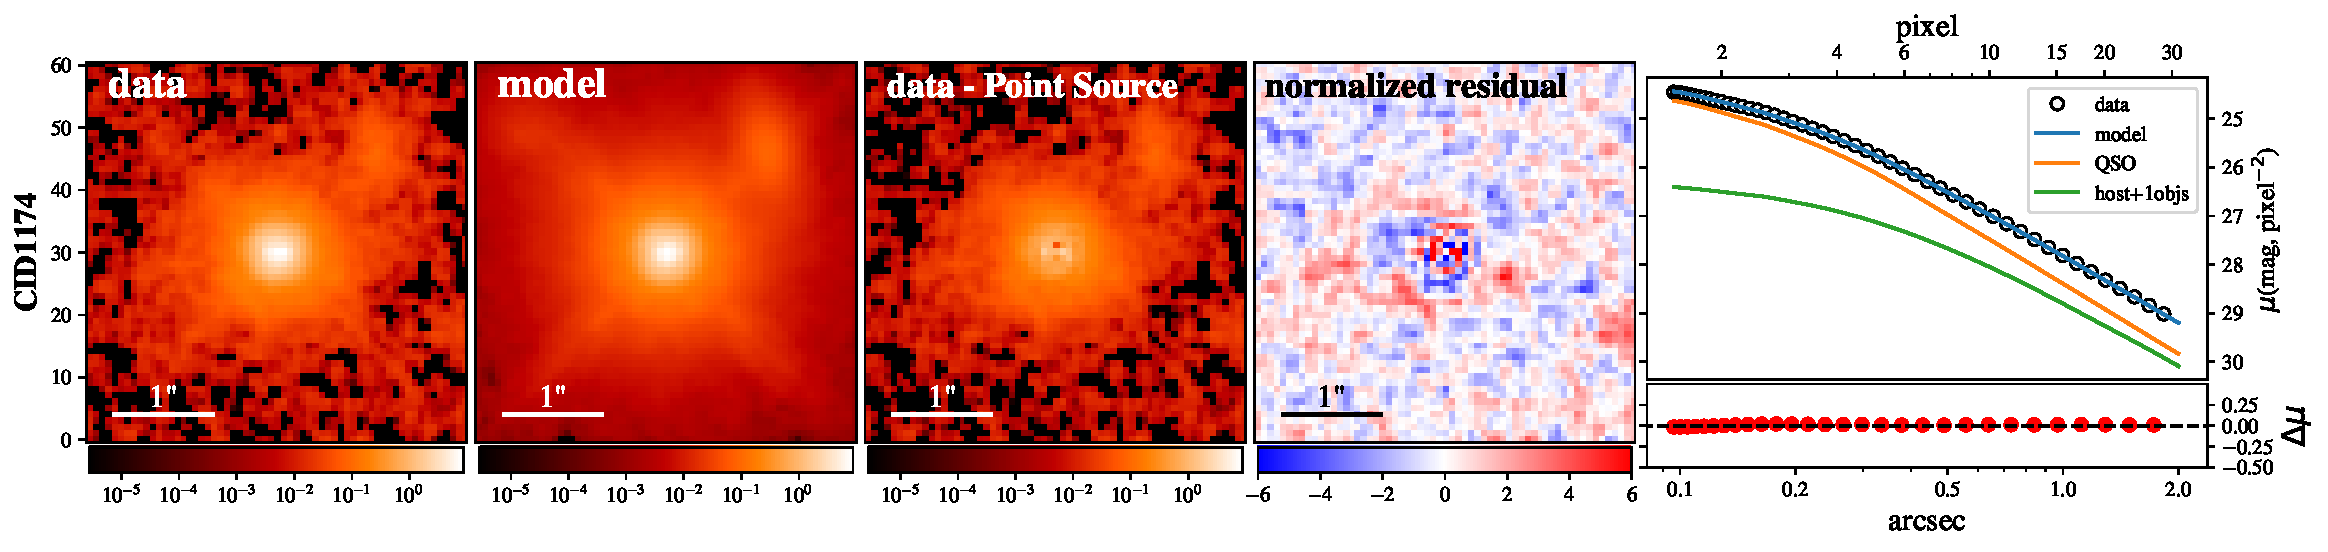
\includegraphics[height=0.25\textwidth]{fig/best_fit_CID1174_SB_profile.pdf}
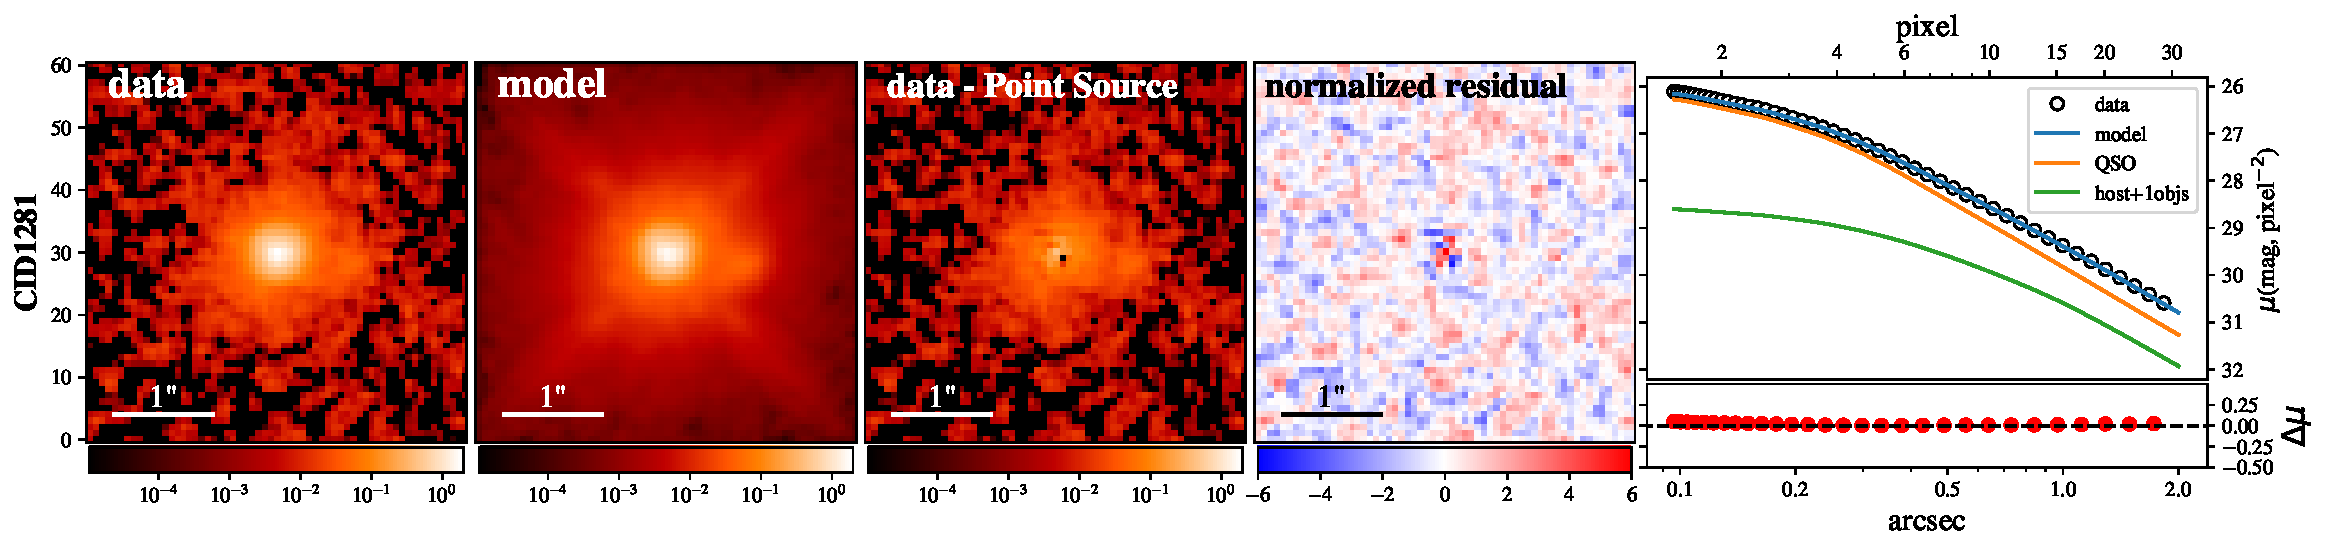
\includegraphics[height=0.25\textwidth]{fig/best_fit_CID1281_SB_profile.pdf}
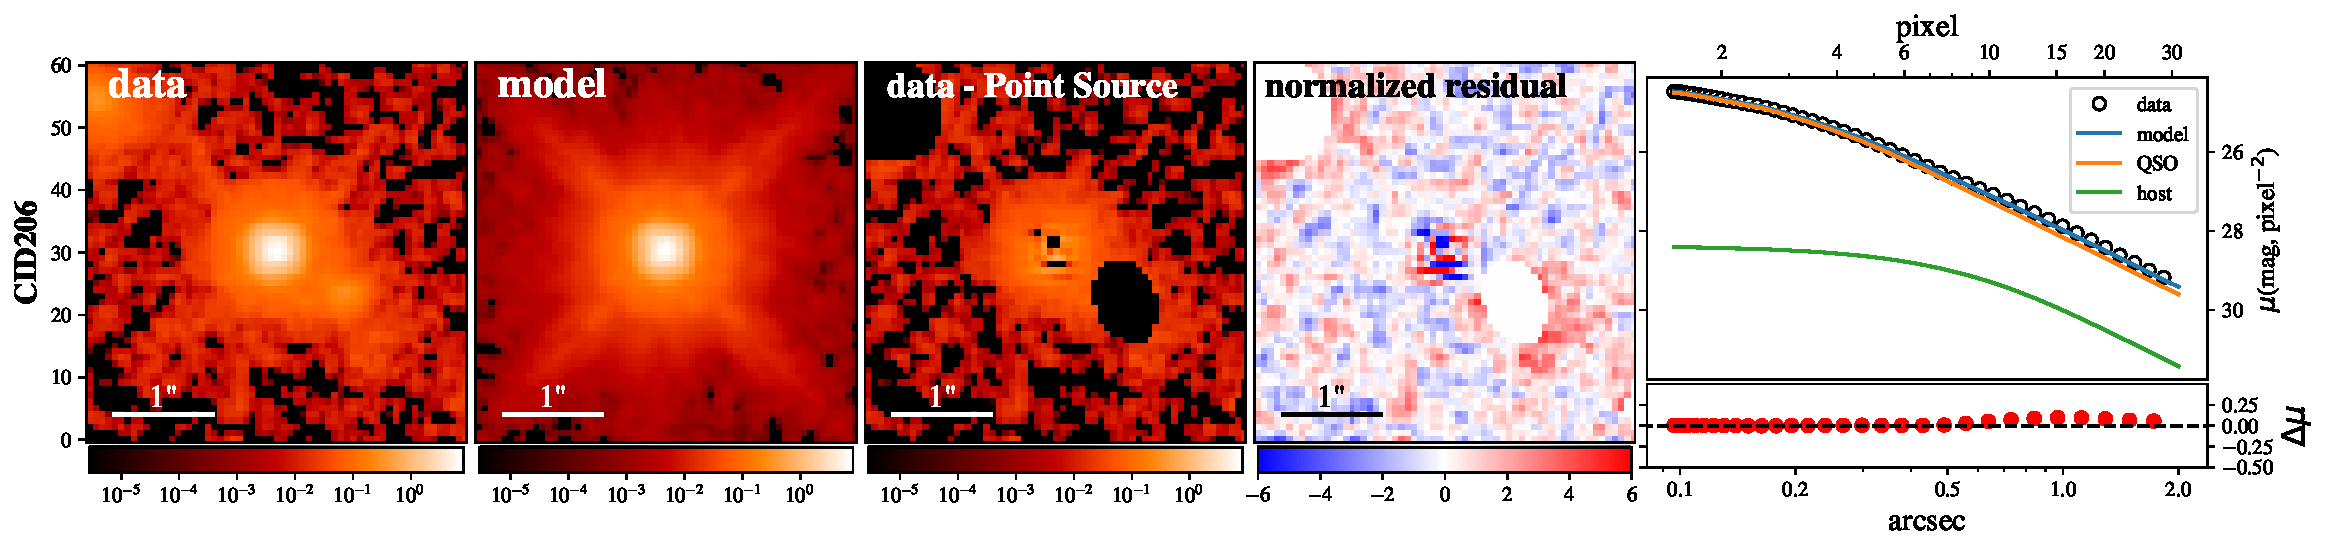
\includegraphics[height=0.25\textwidth]{fig/best_fit_CID206_SB_profile.pdf}
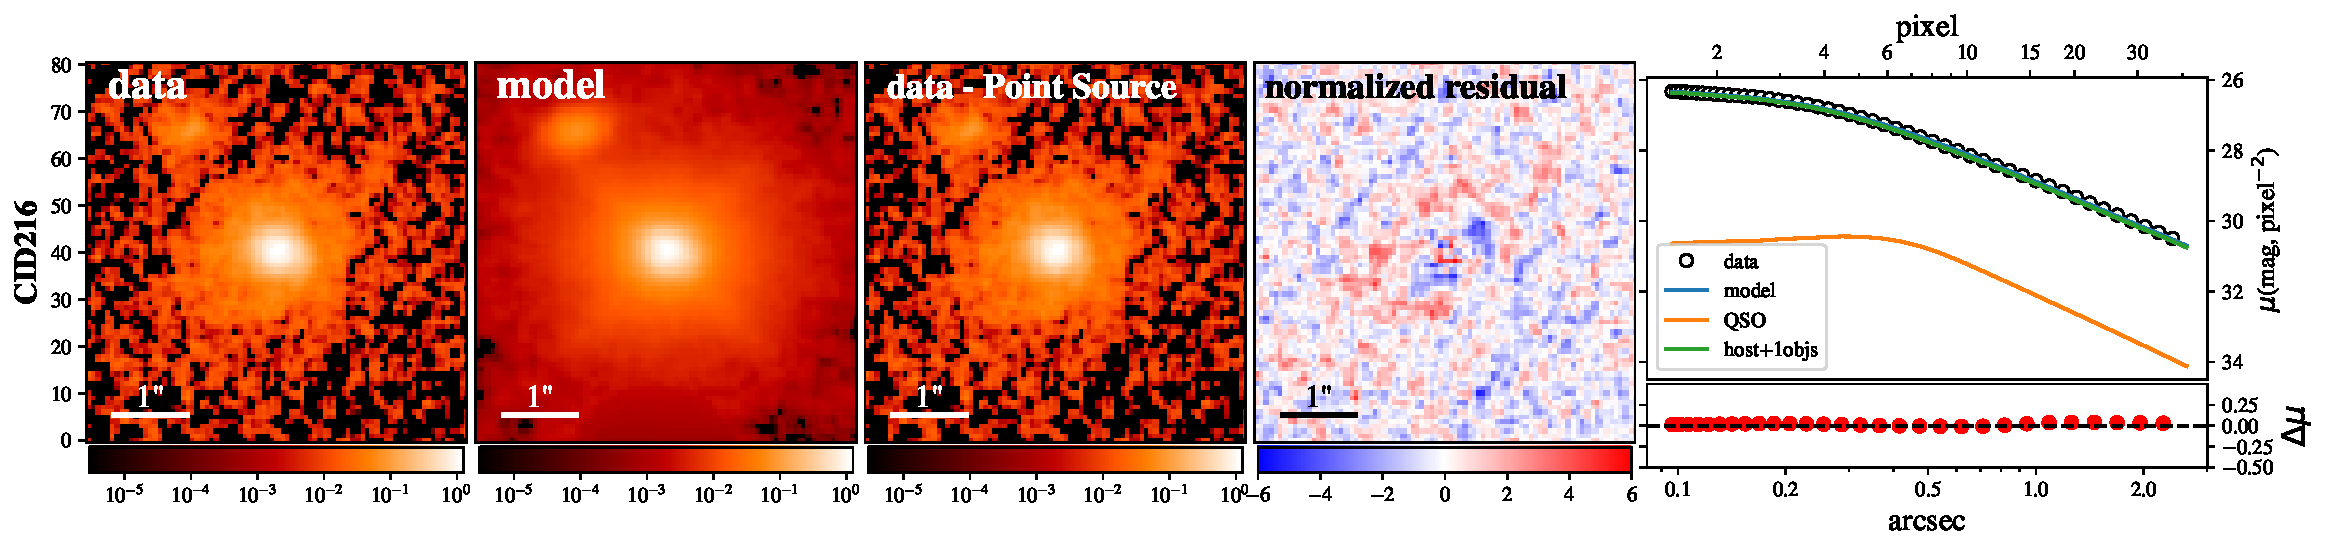
\includegraphics[height=0.25\textwidth]{fig/best_fit_CID216_SB_profile.pdf}
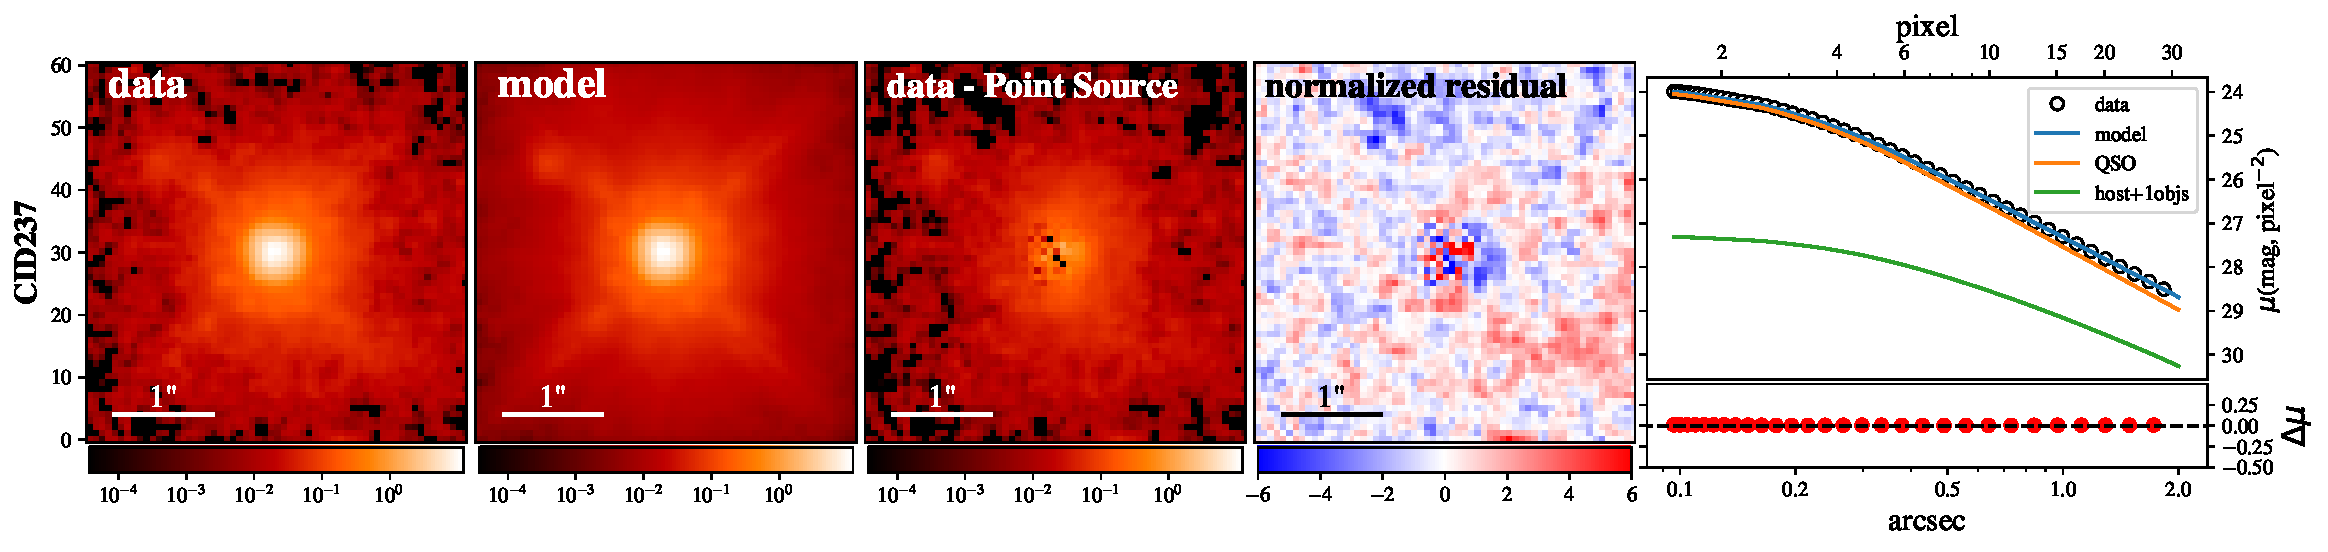
\includegraphics[height=0.25\textwidth]{fig/best_fit_CID237_SB_profile.pdf}
\caption{\label{fig:AGN_decomp} 
Figure illustrates the inference for the 32 objects based on the WFC3 images.
In each row, observed data (first column), best-fit models (second column), data subtracted by the inferred point source (third column),  normalized residuals (fourth column) are presented together with the target ID. In the fifth column, we present the 1-D surface brightness profiles (top) and the corresponding residual (bottom). The 1-D profiles indicate the surface brightness including the data (open circles), the best-fit model (blue line), the AGN (orange line), and the model for the extended sources (green line, i.e., host and other objects). Note that the one-dimensional surface brightness profiles are only for illustration purposes. The actual fitting is based on the two-dimensional images.
}}
\end{figure*} 

\begin{figure*}
\centering
%\hspace{-5.5em}
{
\includegraphics[height=0.25\textwidth]{fig/best_fit_CID255_SB_profile.pdf}
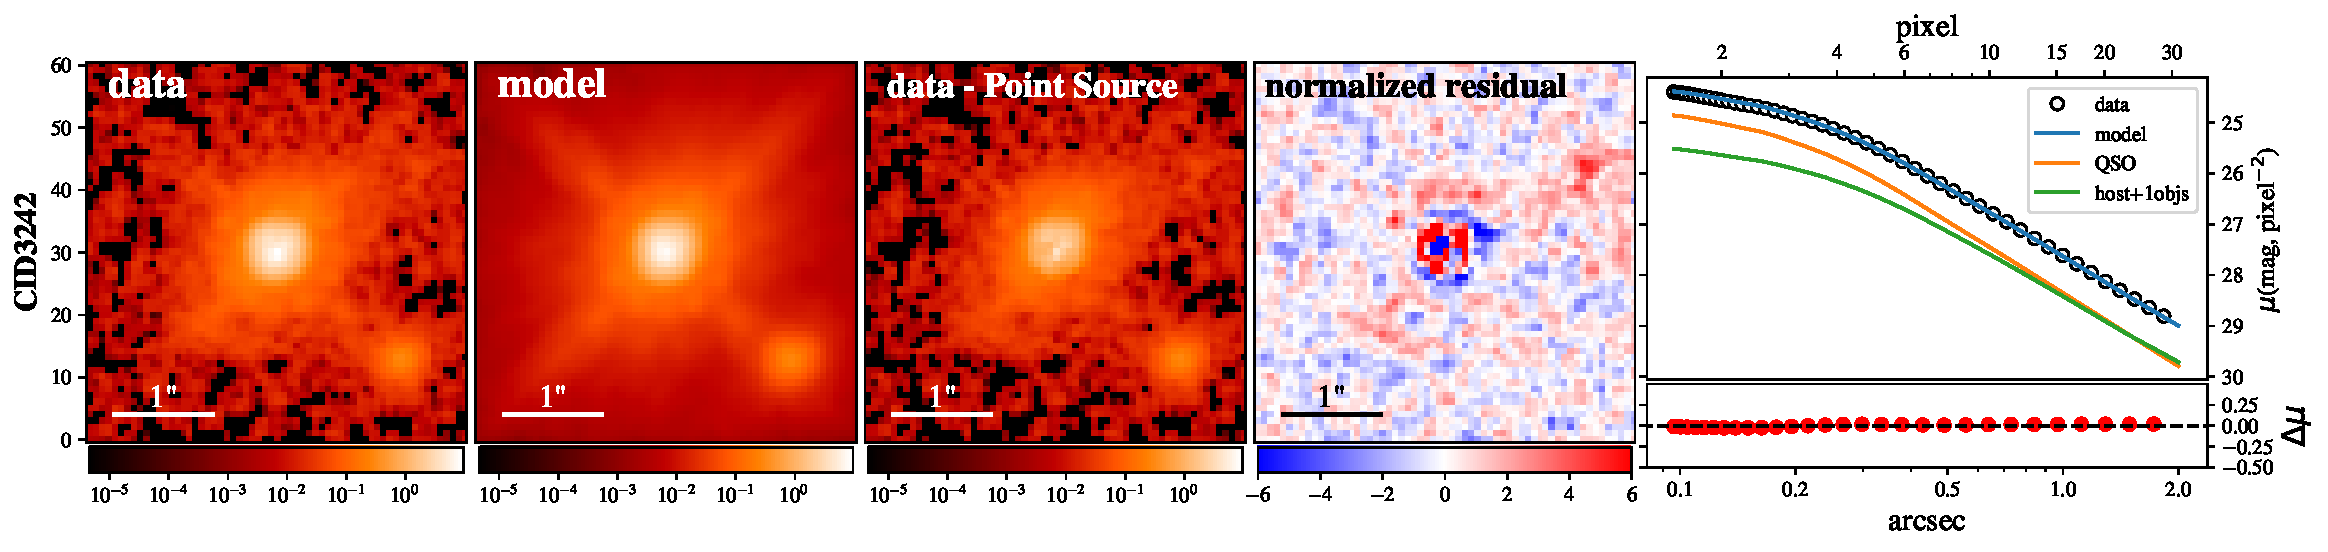
\includegraphics[height=0.25\textwidth]{fig/best_fit_CID3242_SB_profile.pdf}
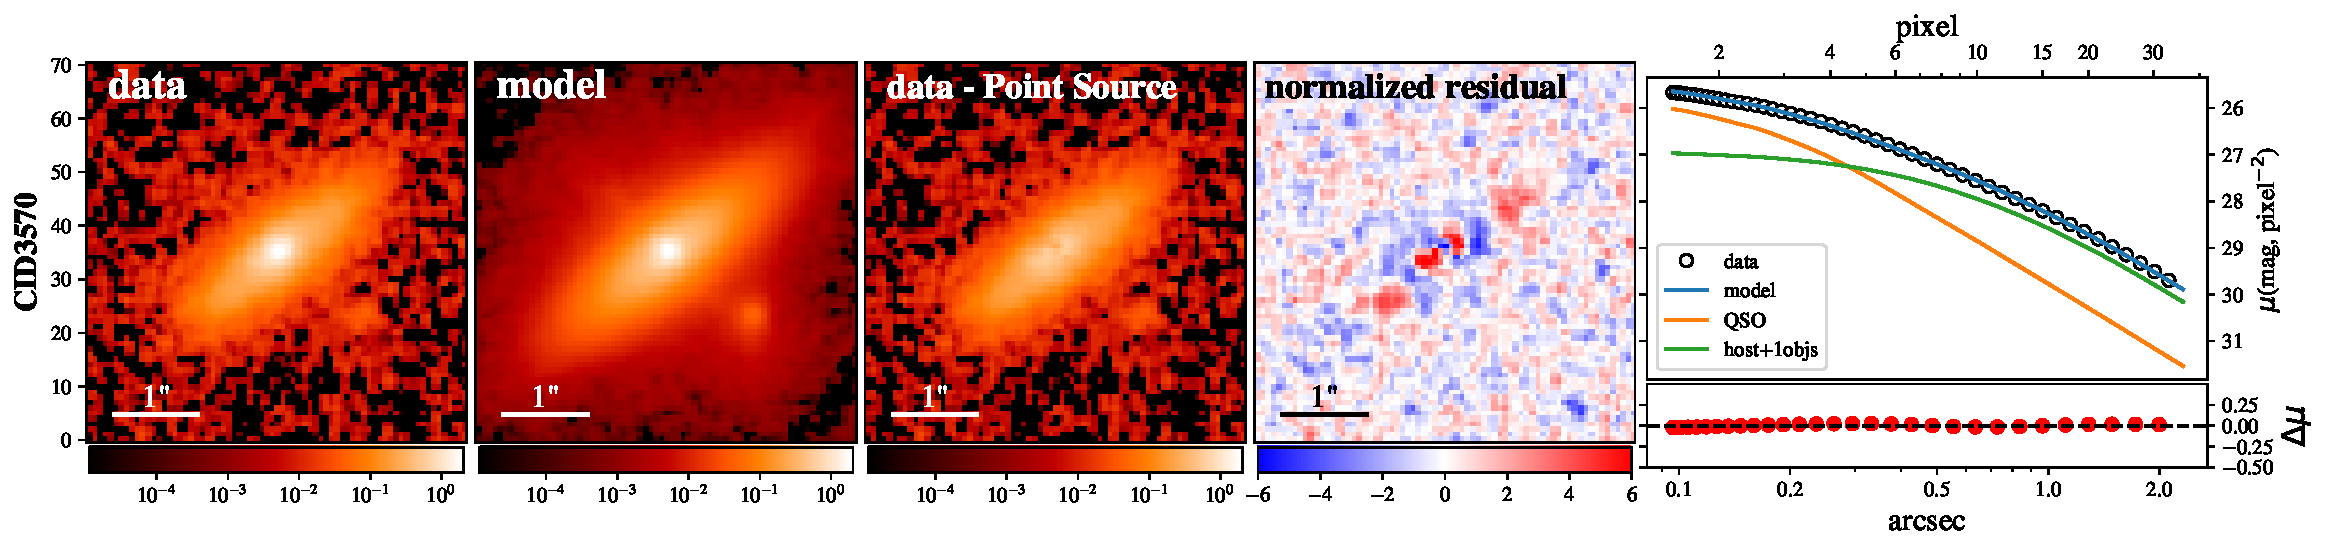
\includegraphics[height=0.25\textwidth]{fig/best_fit_CID3570_SB_profile.pdf}
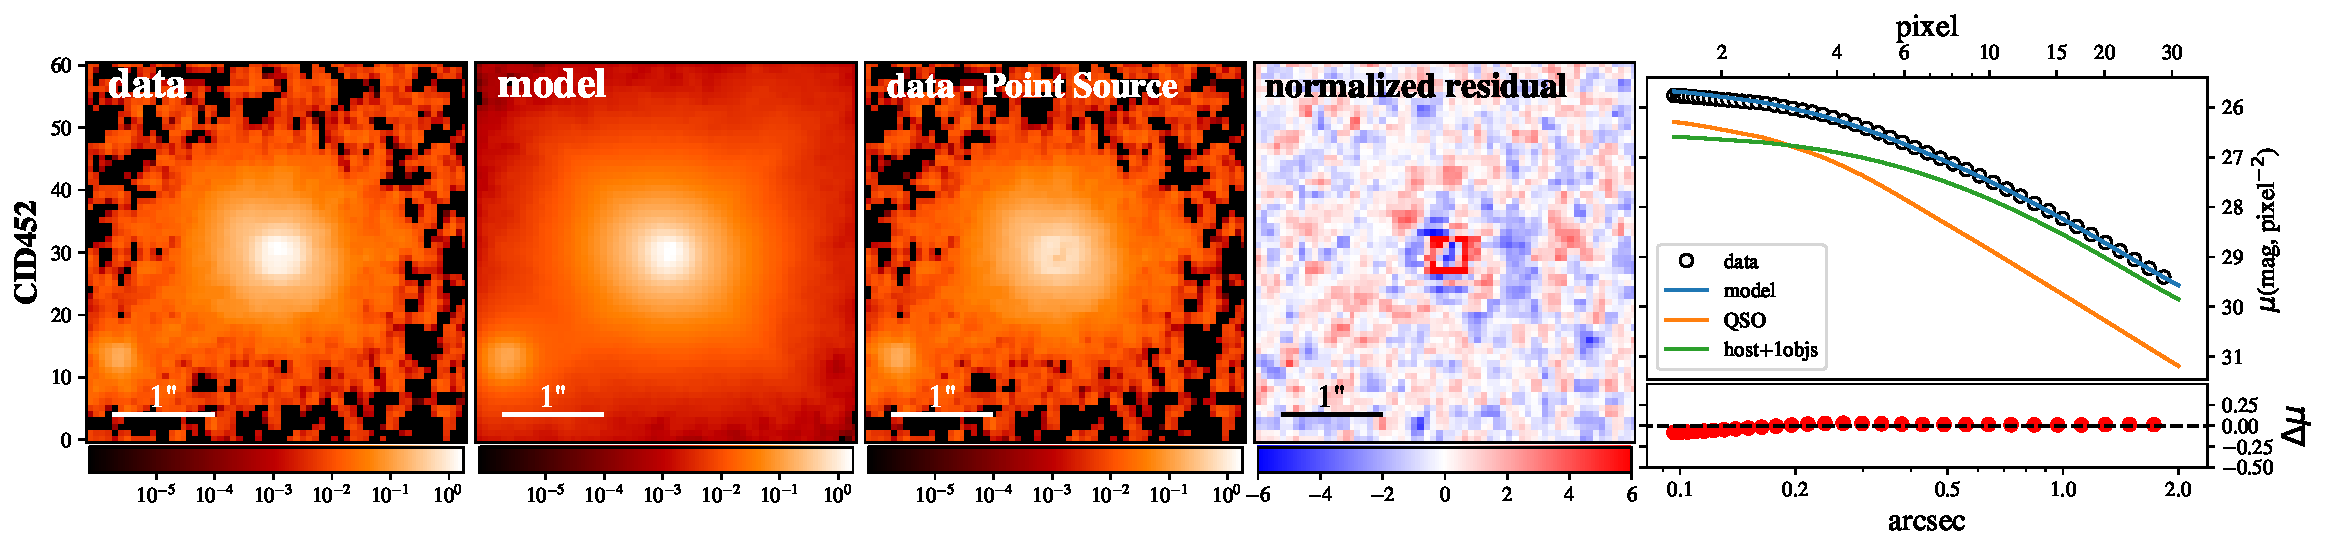
\includegraphics[height=0.25\textwidth]{fig/best_fit_CID452_SB_profile.pdf}
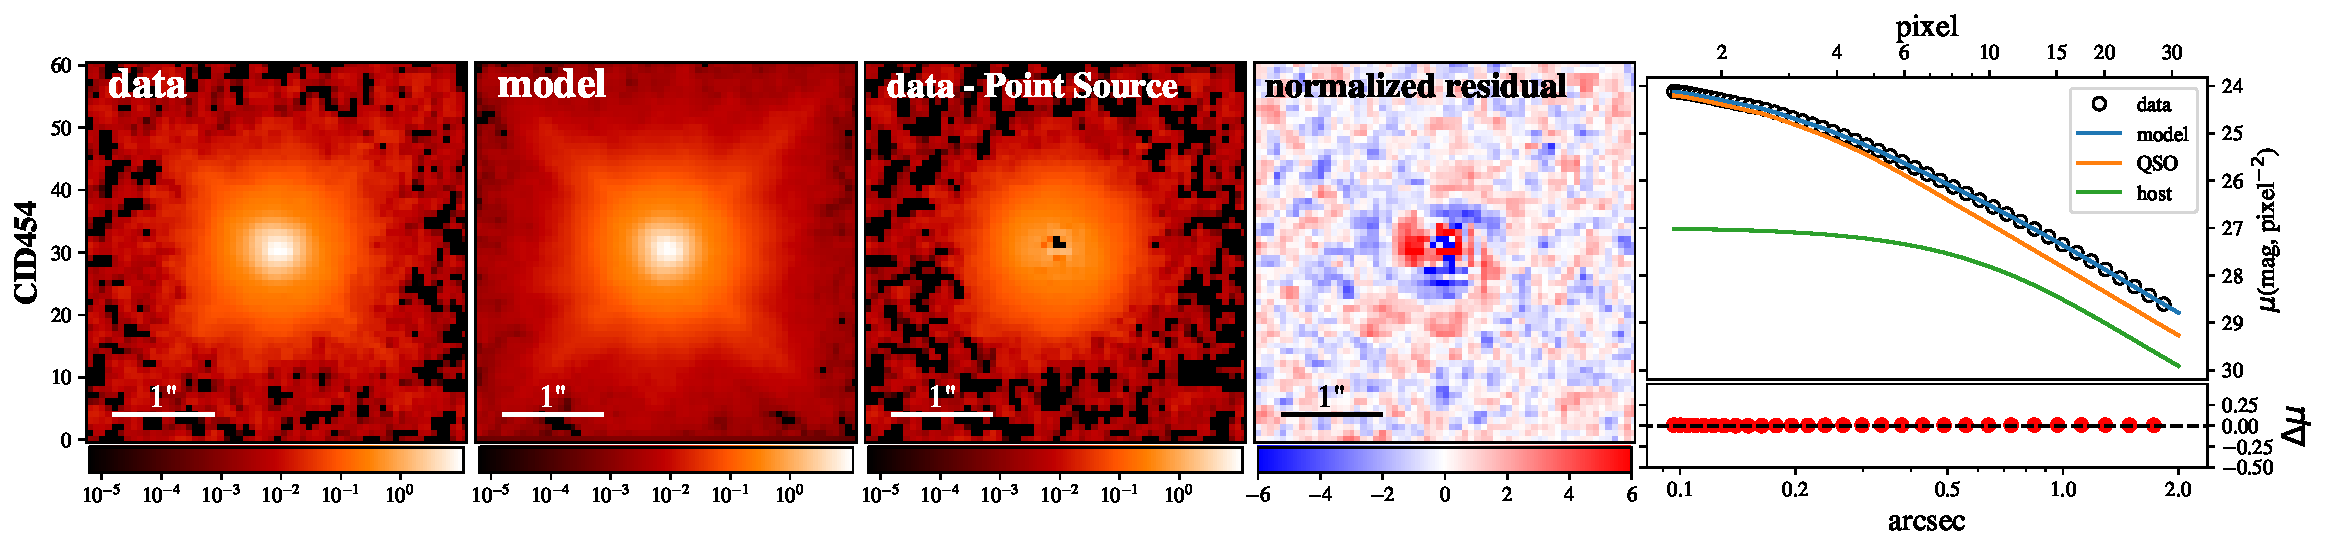
\includegraphics[height=0.25\textwidth]{fig/best_fit_CID454_SB_profile.pdf}
}
\figurenum{1}
\caption{Continued.}
\end{figure*} 

\begin{figure*}
\centering
%\hspace{-5.5em}
{
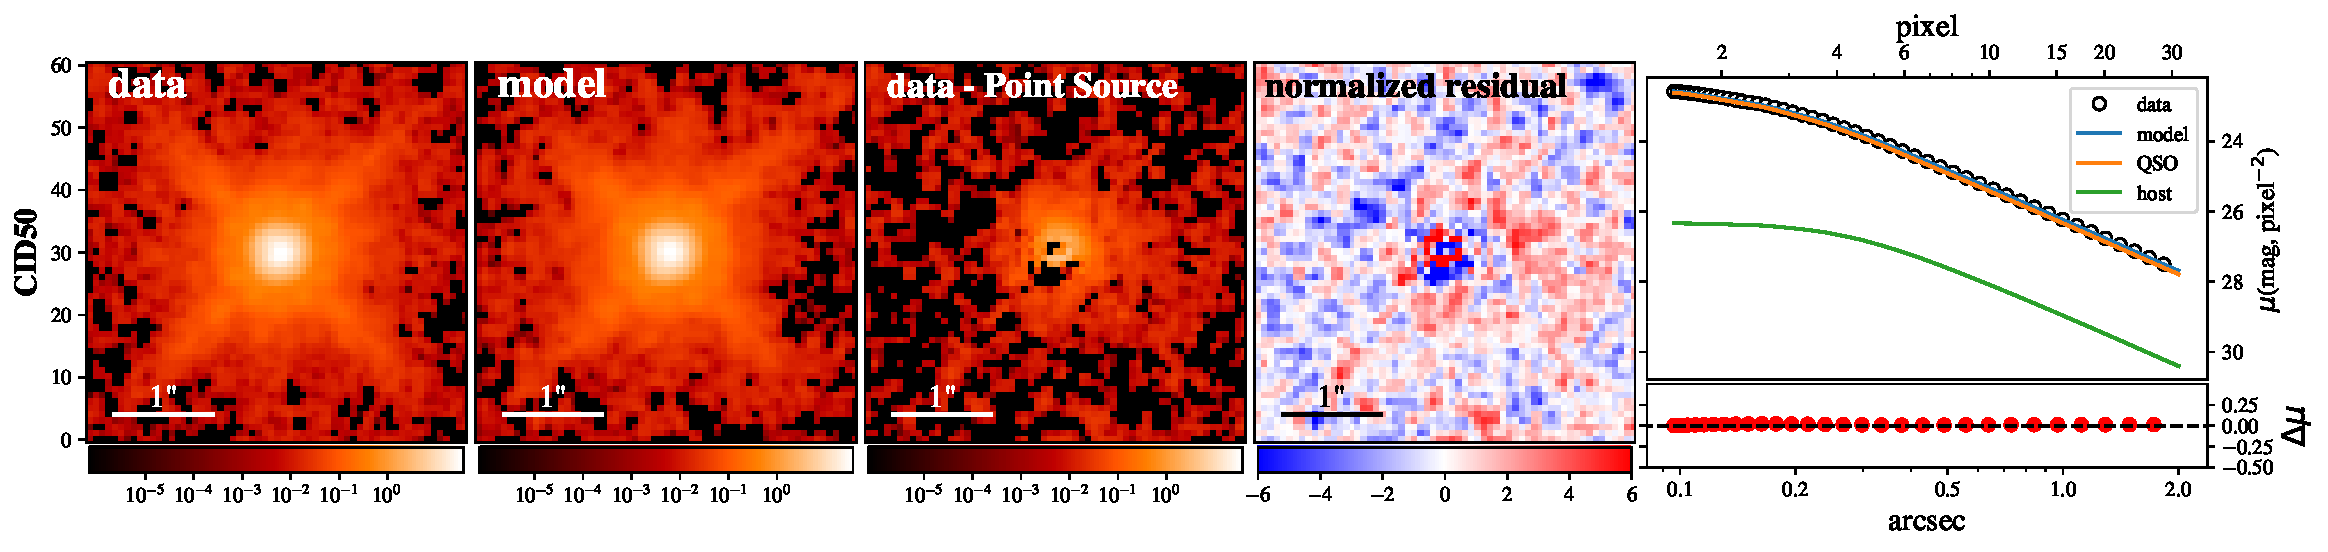
\includegraphics[height=0.25\textwidth]{fig/best_fit_CID50_SB_profile.pdf}
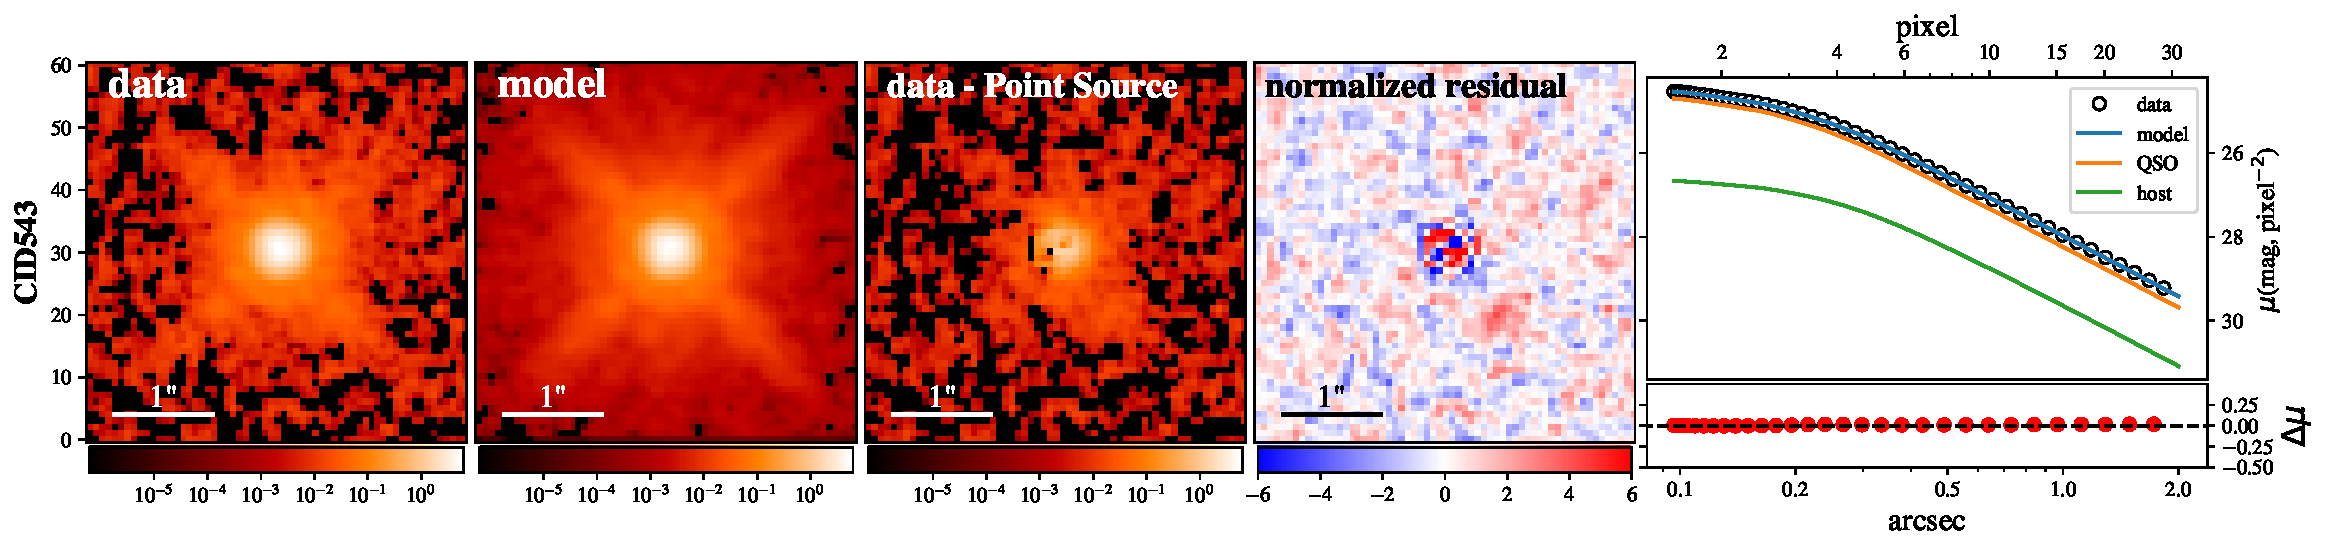
\includegraphics[height=0.25\textwidth]{fig/best_fit_CID543_SB_profile.pdf}
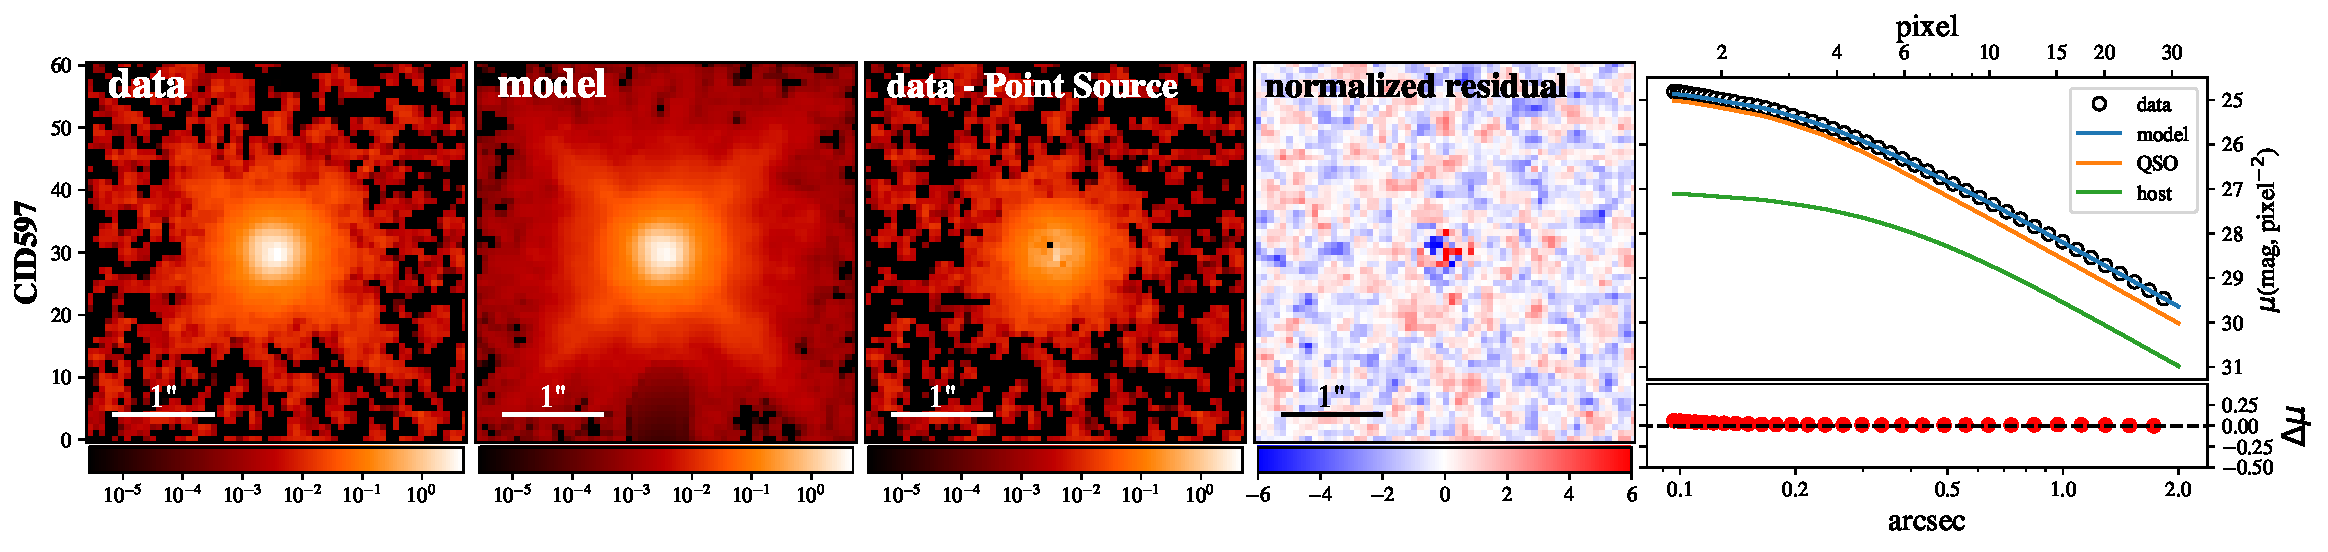
\includegraphics[height=0.25\textwidth]{fig/best_fit_CID597_SB_profile.pdf}
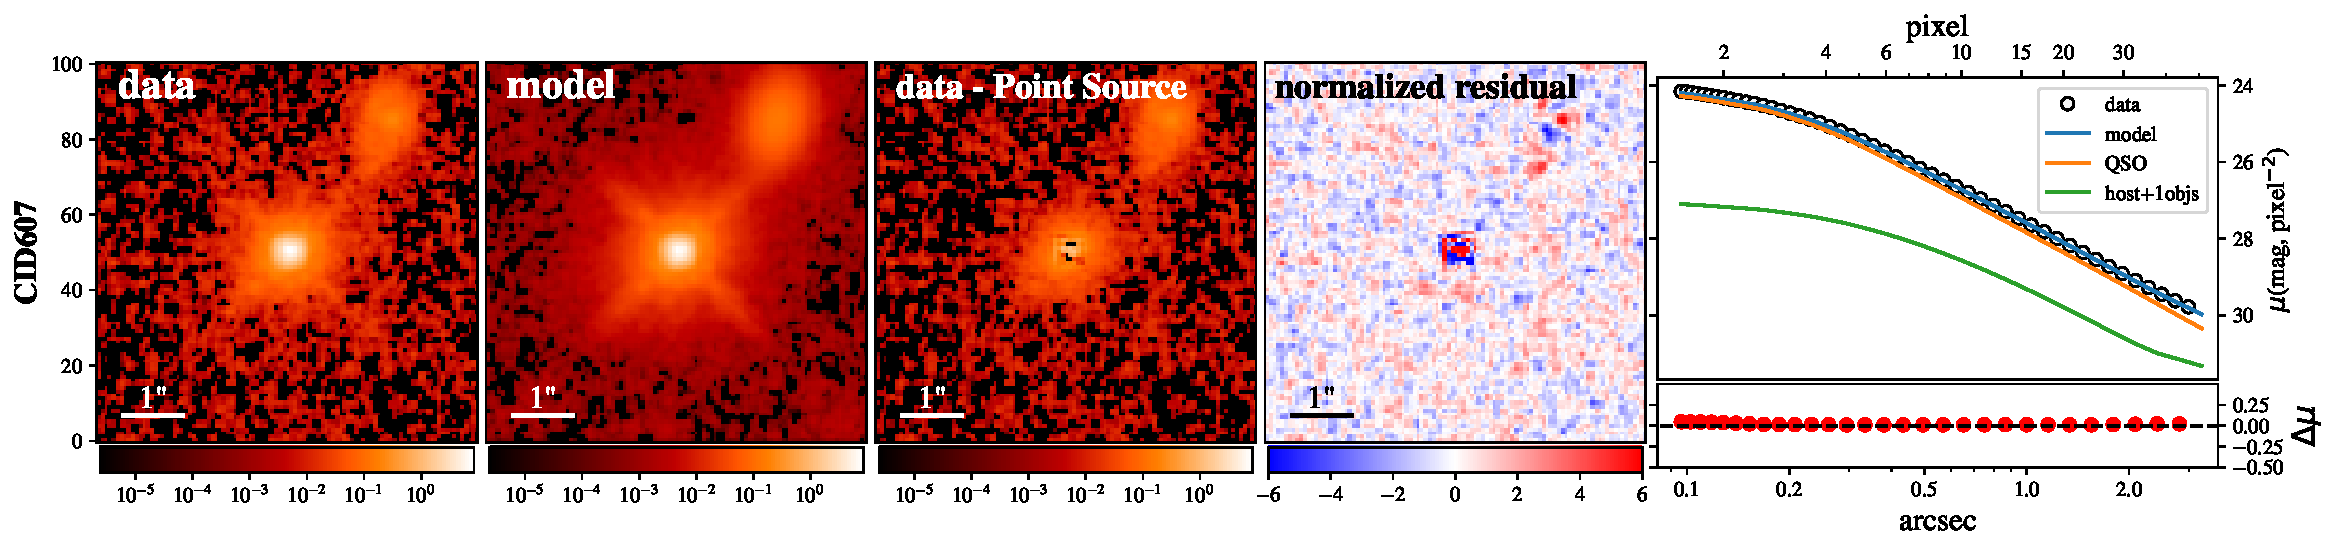
\includegraphics[height=0.25\textwidth]{fig/best_fit_CID607_SB_profile.pdf}
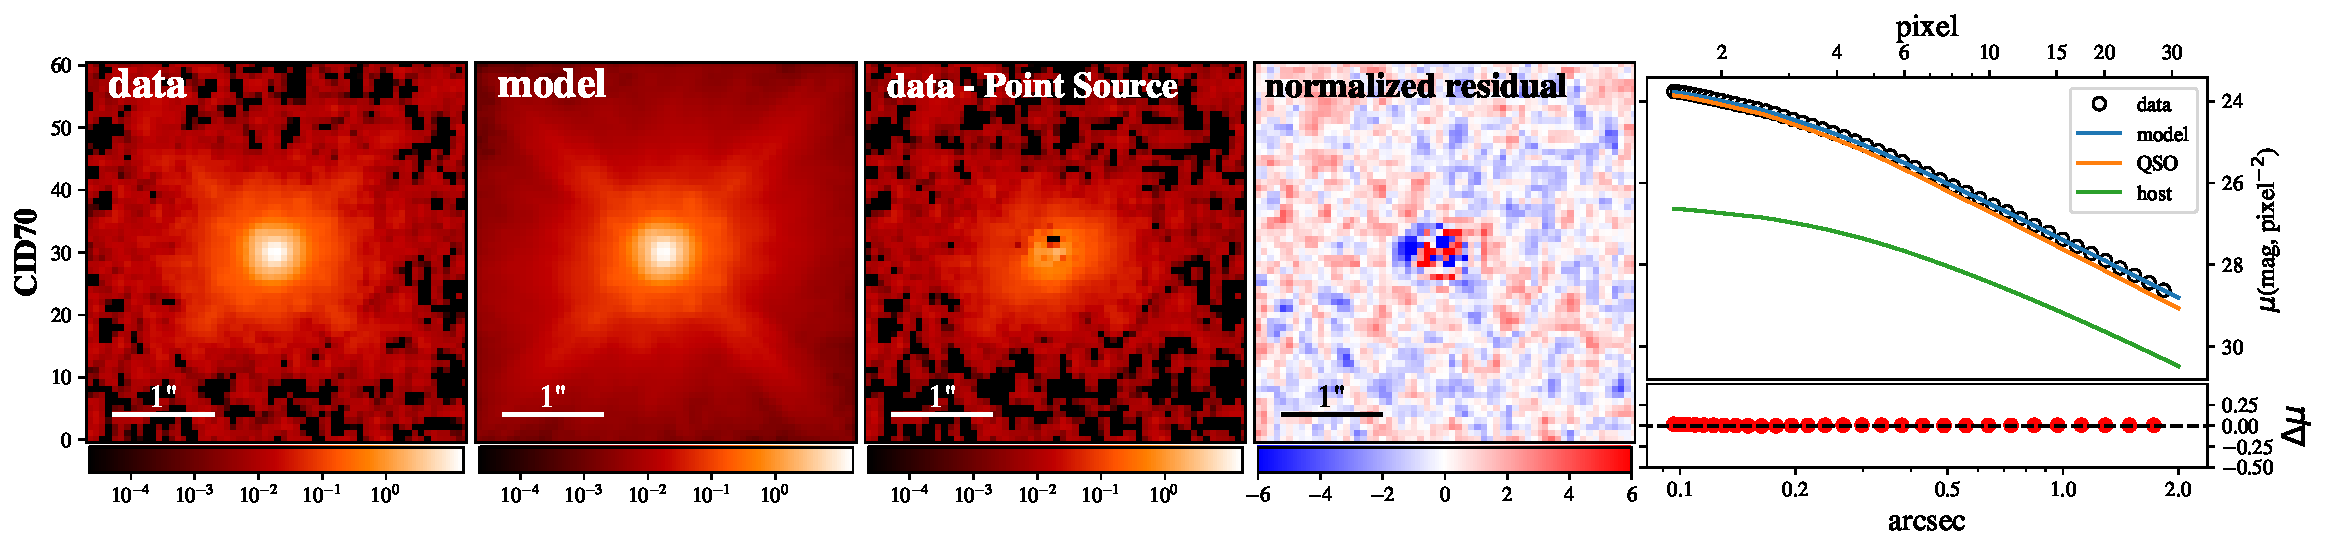
\includegraphics[height=0.25\textwidth]{fig/best_fit_CID70_SB_profile.pdf}
}
\figurenum{1}
\caption{Continued.}
\end{figure*} 

\begin{figure*}
\centering
%\hspace{-5.5em}
{
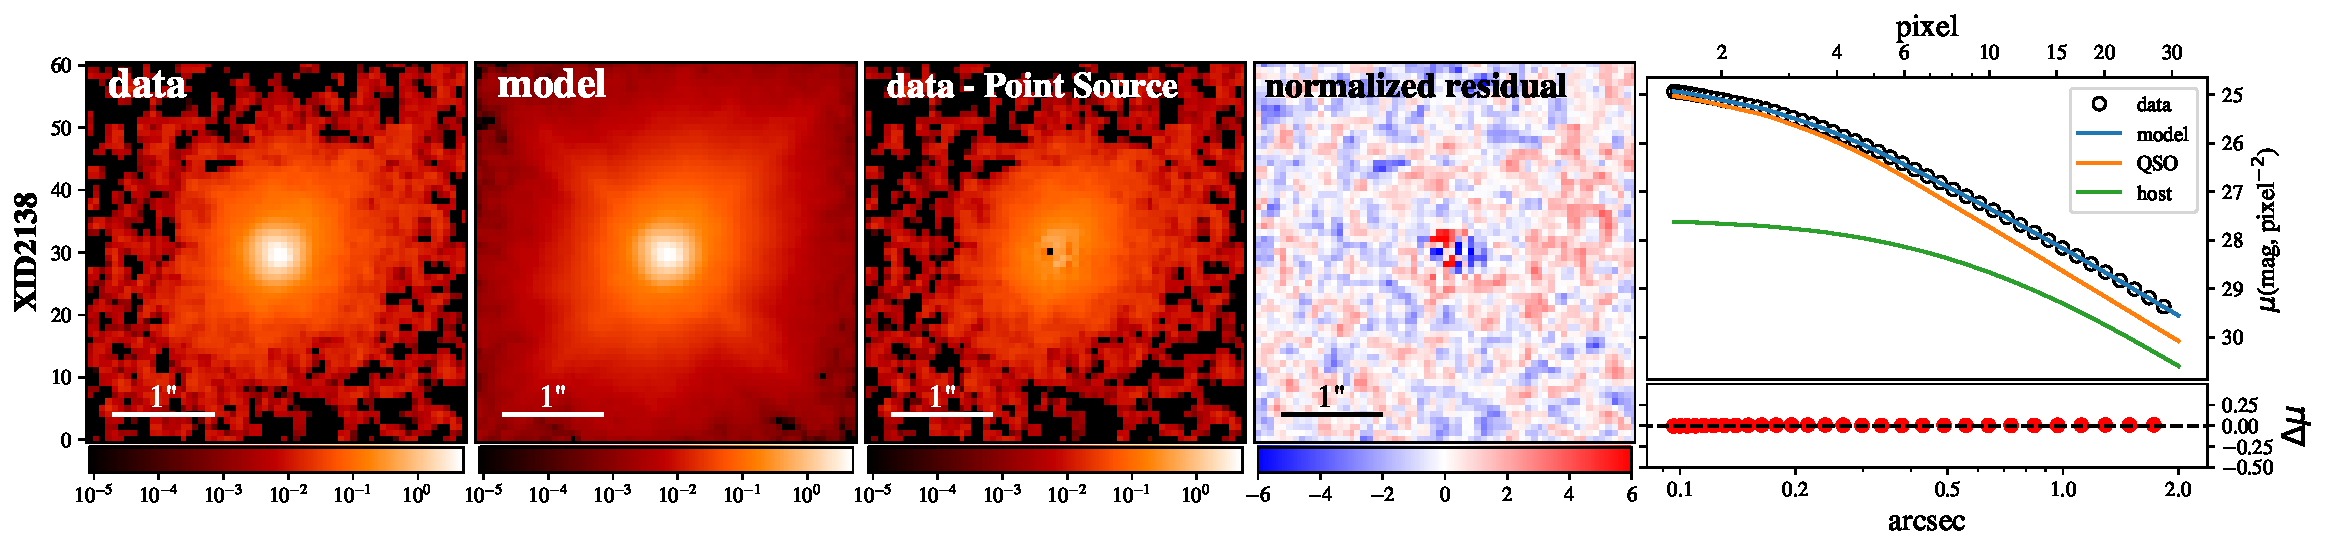
\includegraphics[height=0.25\textwidth]{fig/best_fit_XID2138_SB_profile.pdf}
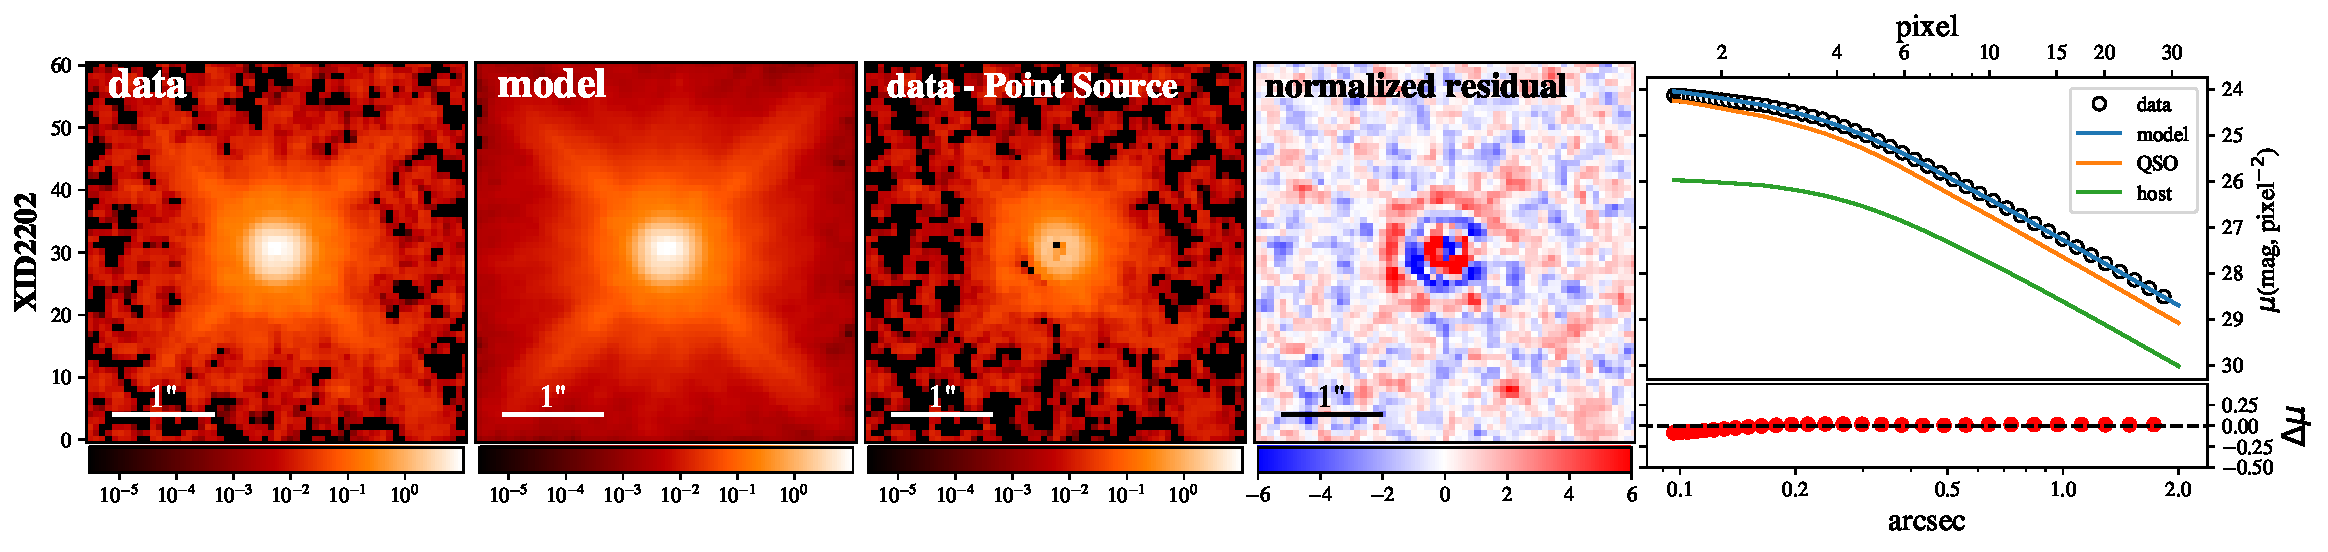
\includegraphics[height=0.25\textwidth]{fig/best_fit_XID2202_SB_profile.pdf}
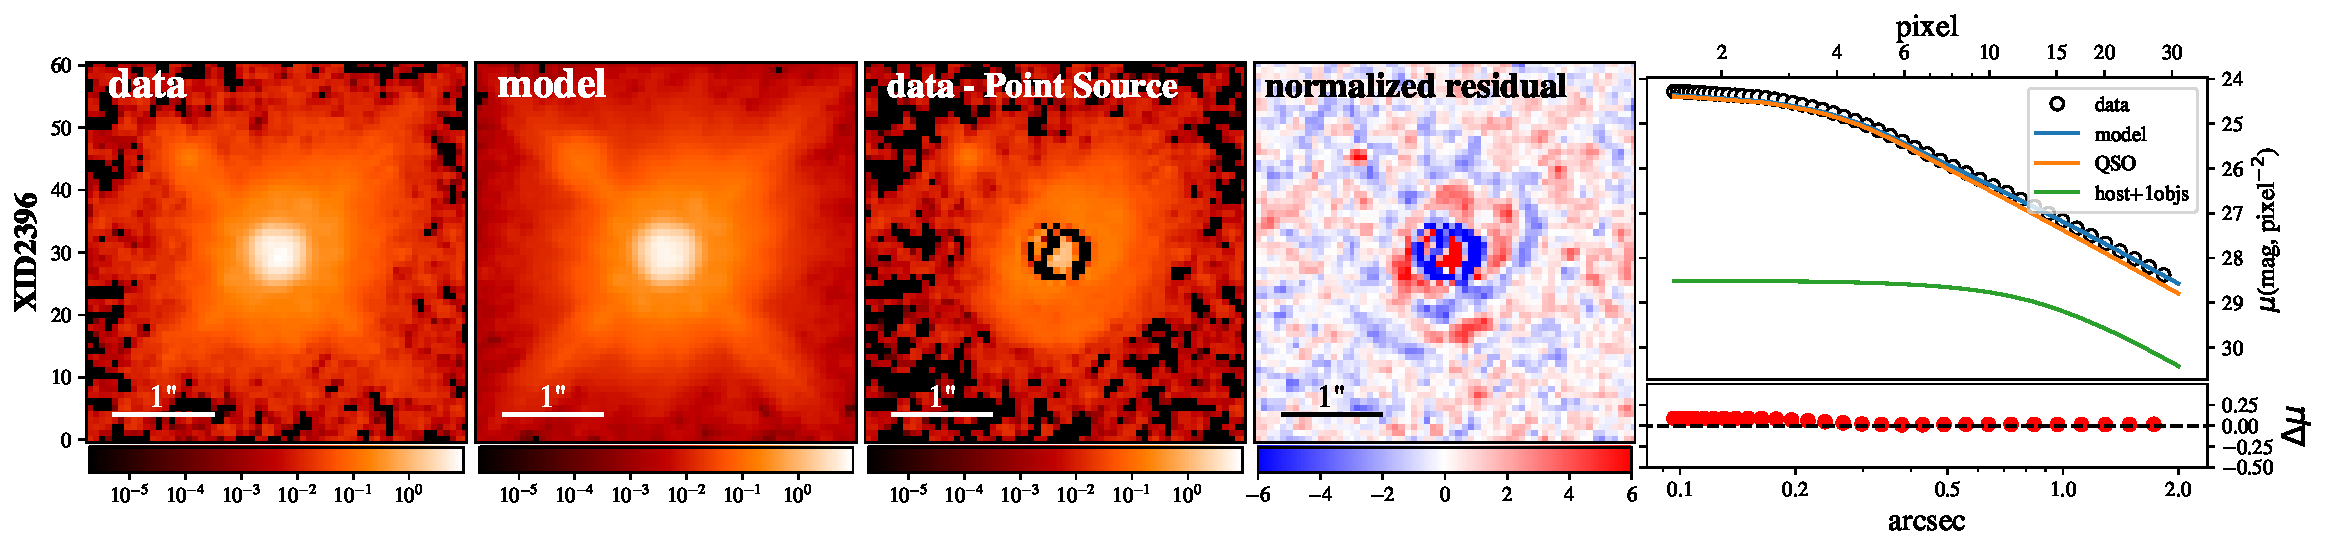
\includegraphics[height=0.25\textwidth]{fig/best_fit_XID2396_SB_profile.pdf}
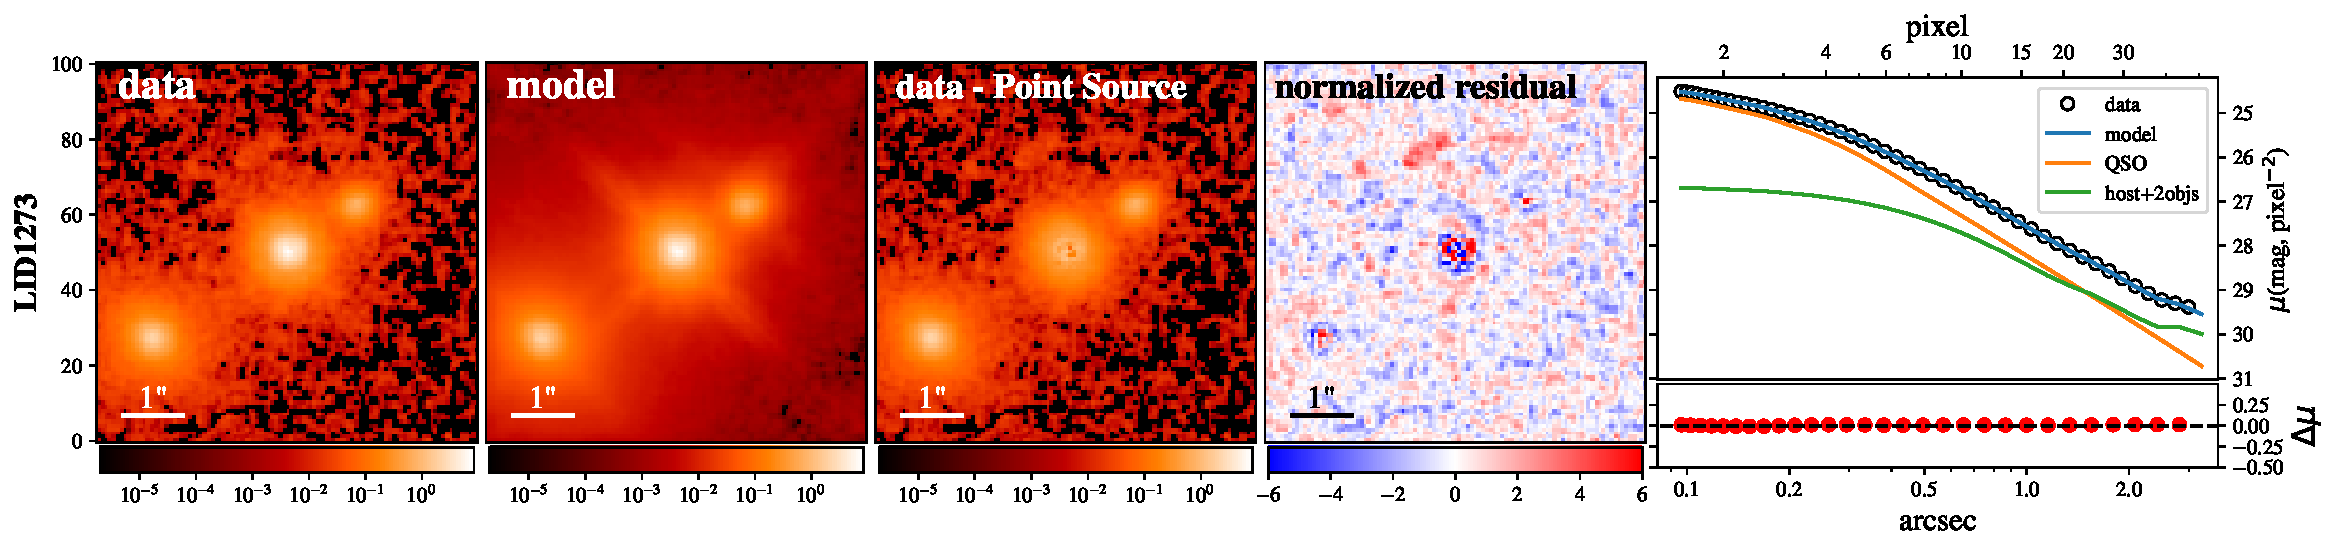
\includegraphics[height=0.25\textwidth]{fig/best_fit_LID1273_SB_profile.pdf}
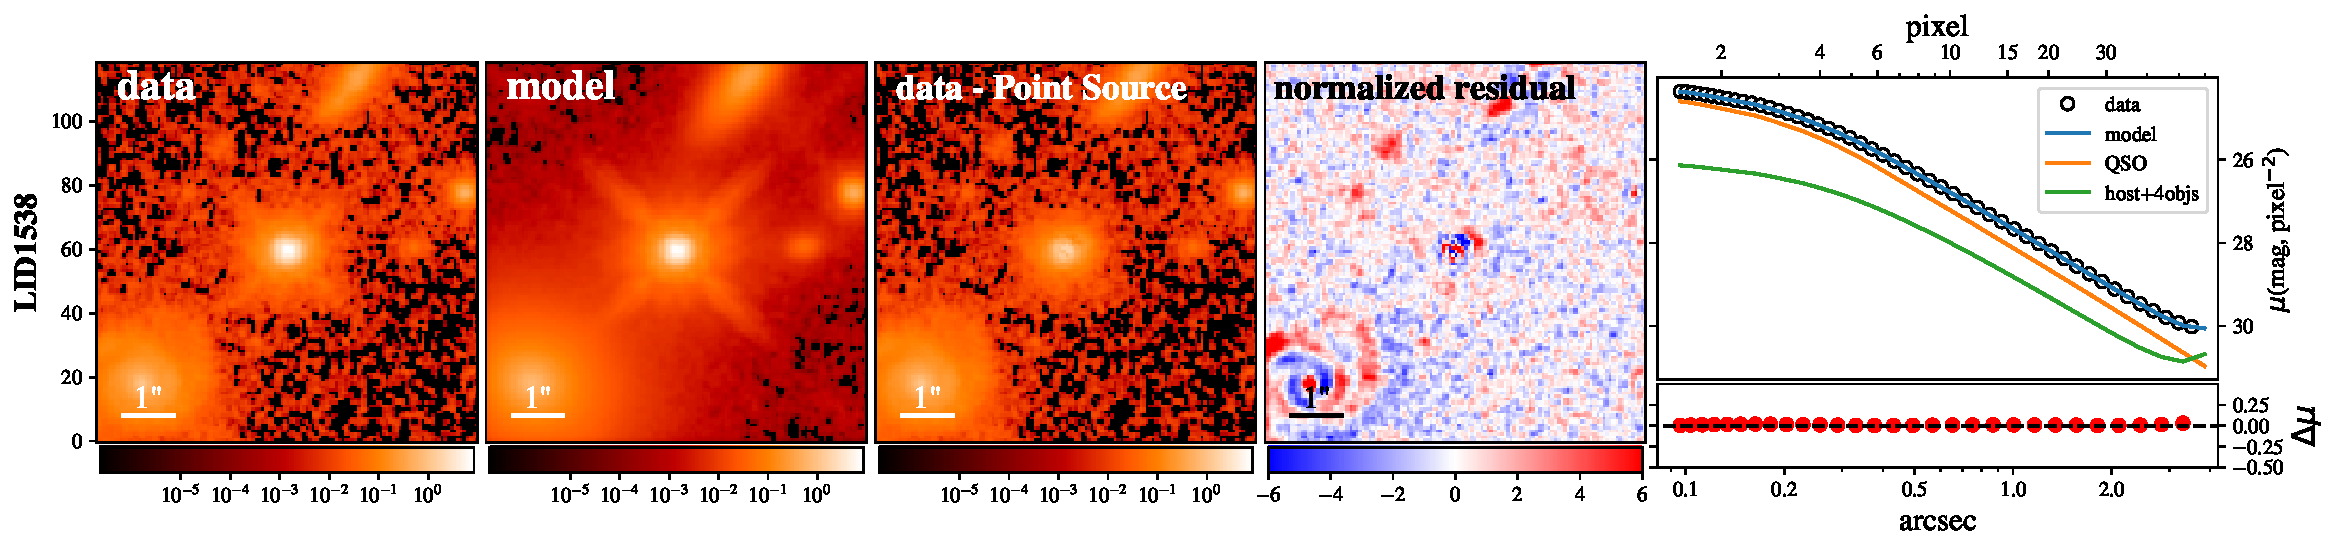
\includegraphics[height=0.25\textwidth]{fig/best_fit_LID1538_SB_profile.pdf}
}
\figurenum{1}
\caption{Continued.}
\end{figure*} 

\begin{figure*}
\centering
%\hspace{-5.5em}
{
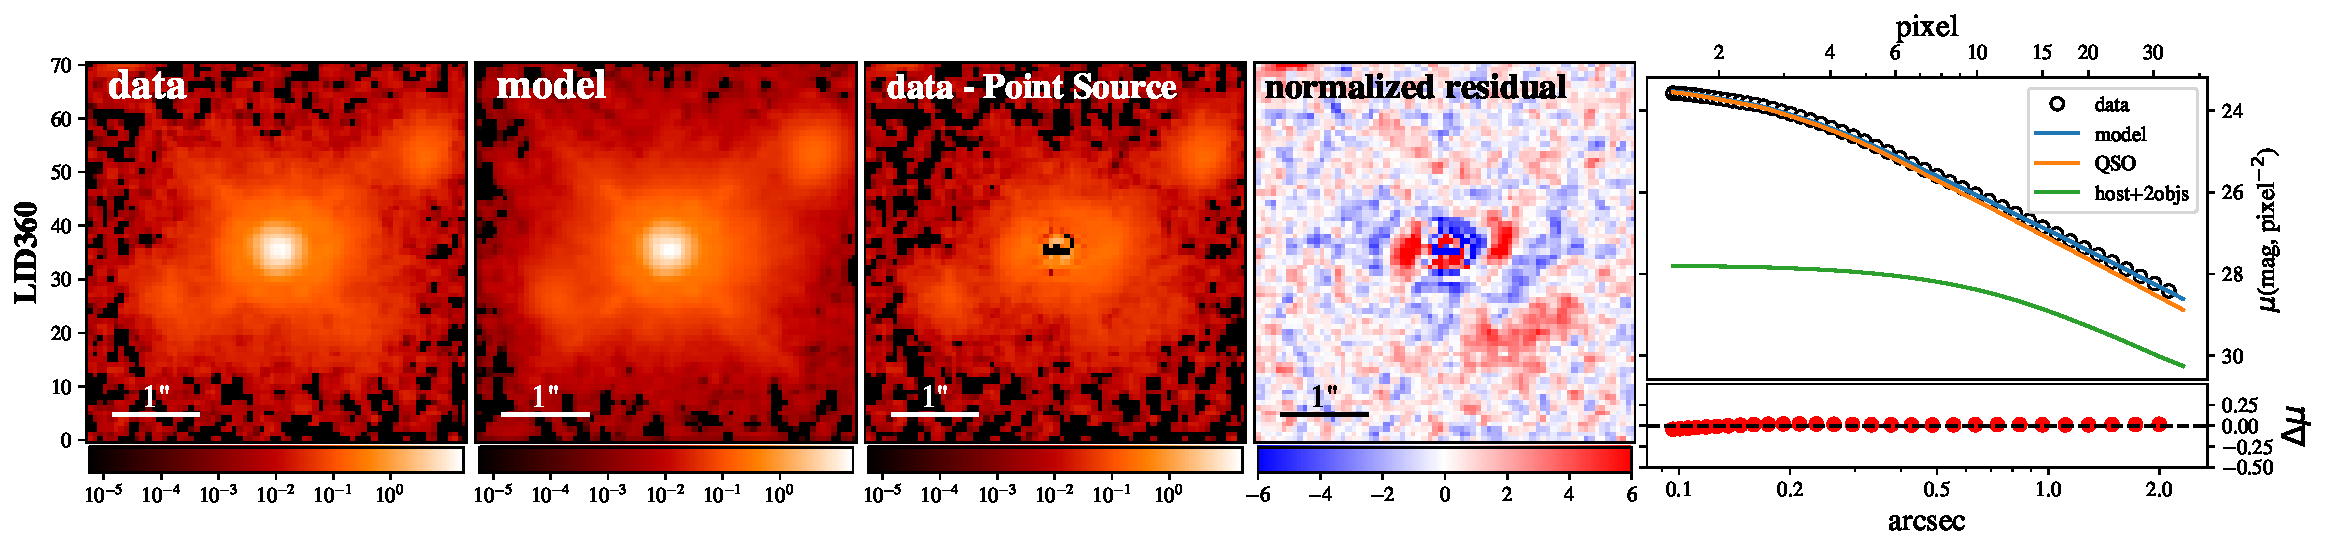
\includegraphics[height=0.25\textwidth]{fig/best_fit_LID360_SB_profile.pdf}
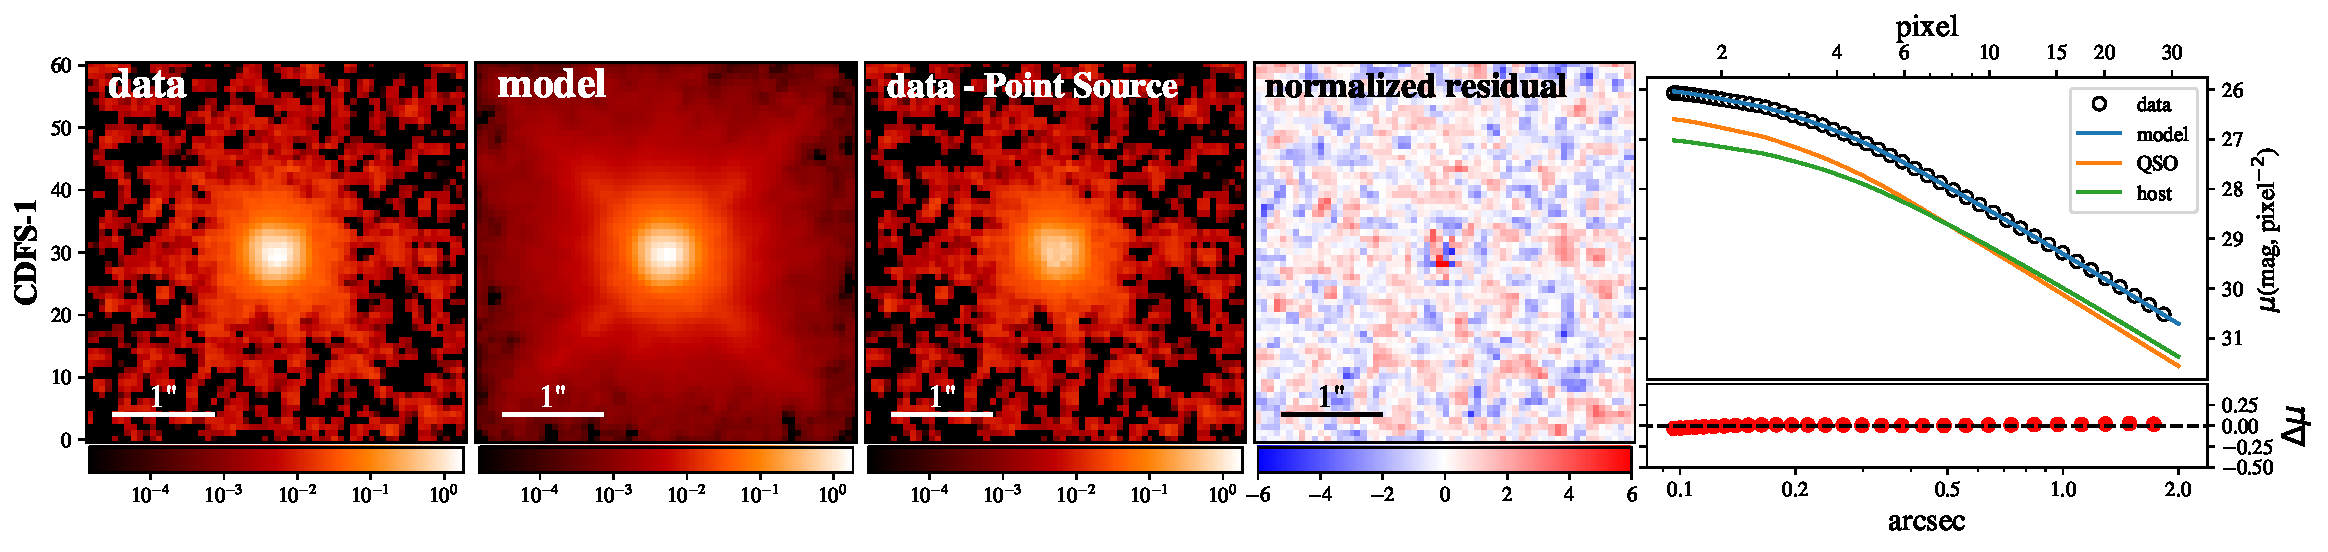
\includegraphics[height=0.25\textwidth]{fig/best_fit_CDFS-1_SB_profile.pdf}
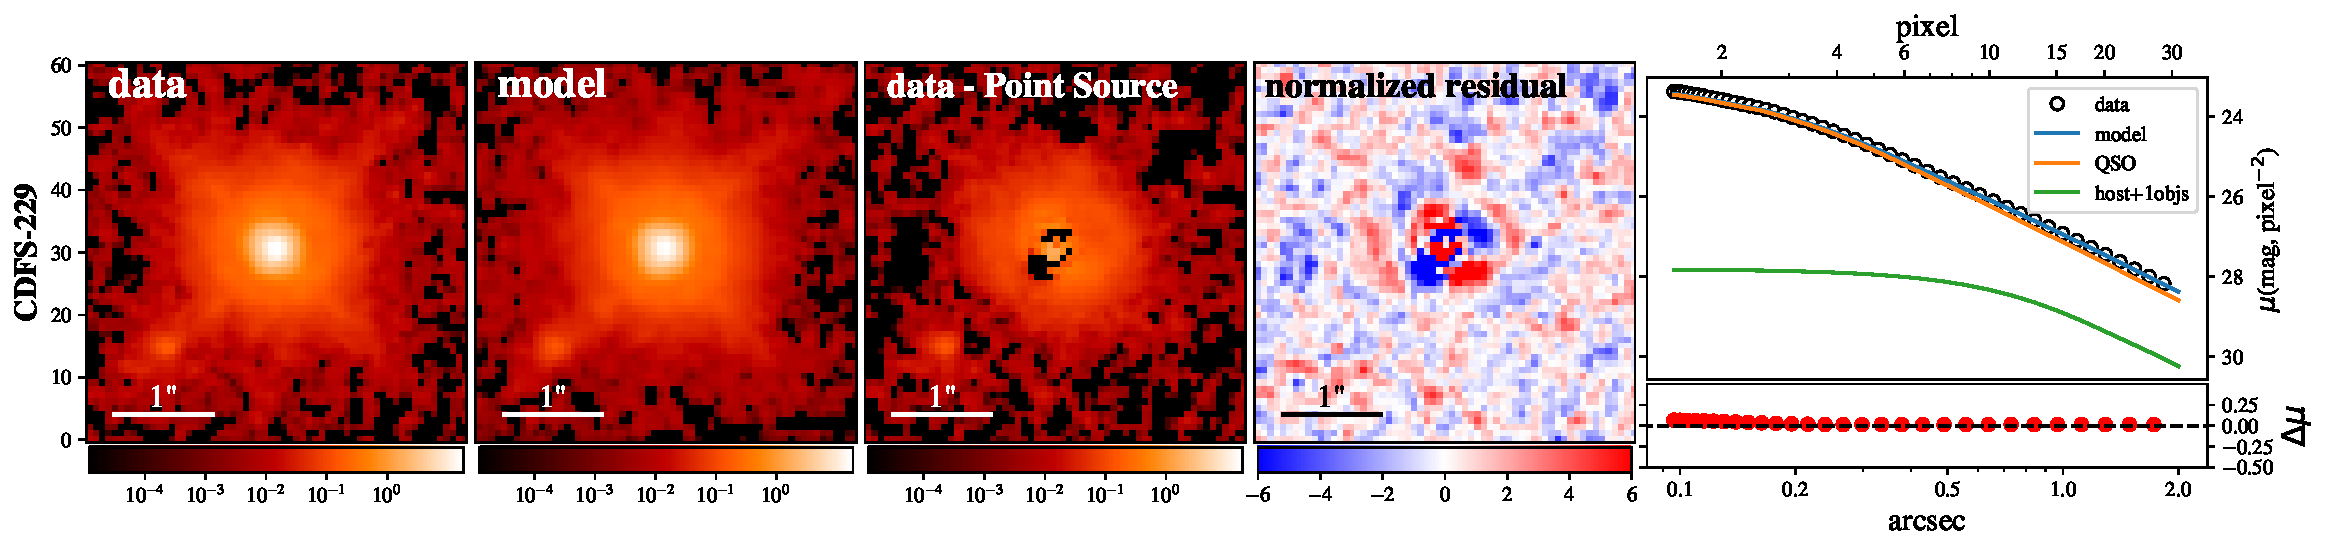
\includegraphics[height=0.25\textwidth]{fig/best_fit_CDFS-229_SB_profile.pdf}
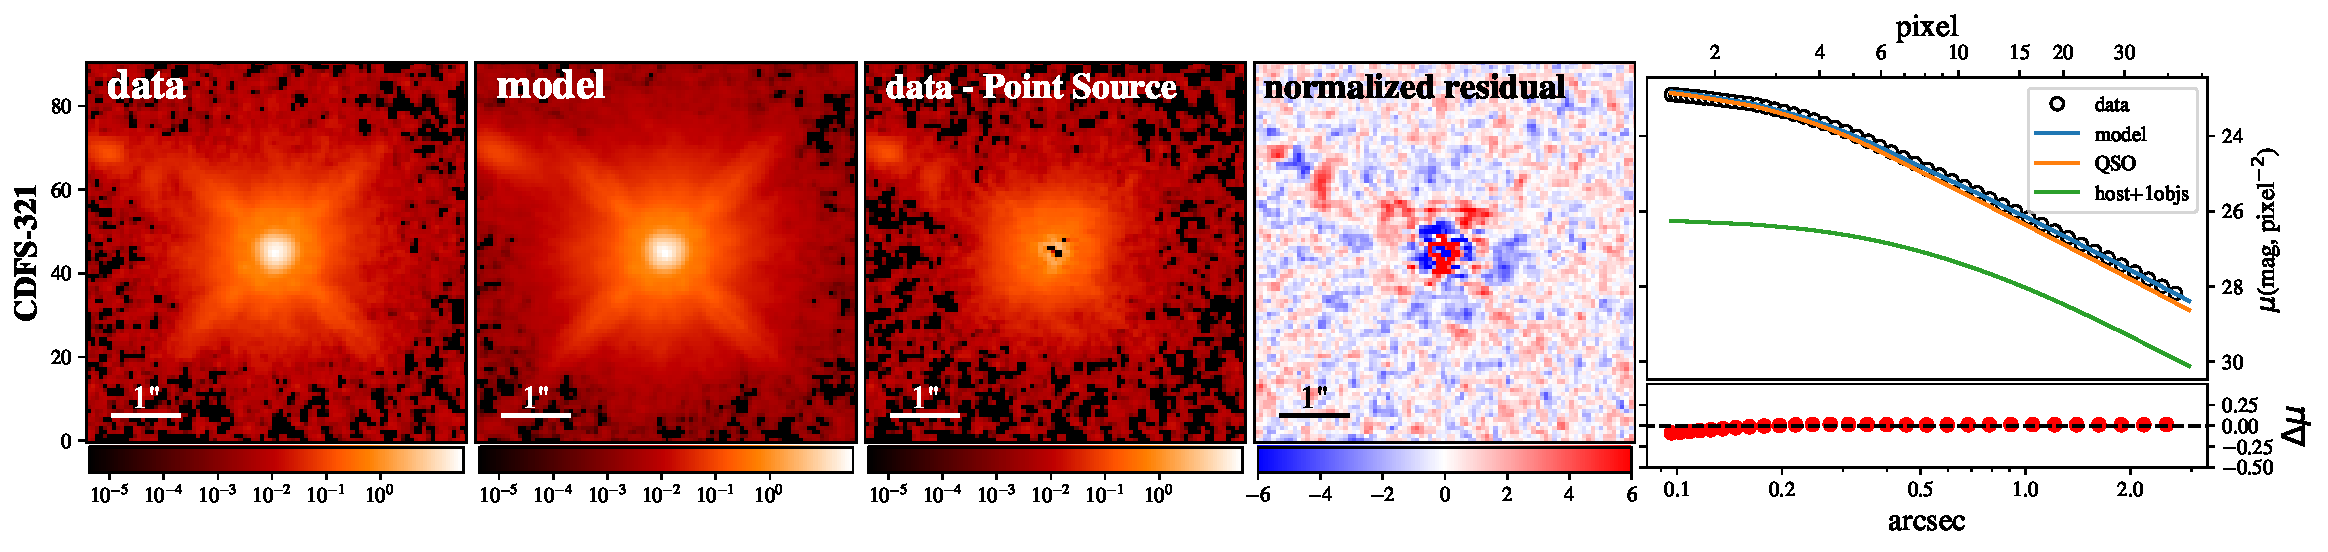
\includegraphics[height=0.25\textwidth]{fig/best_fit_CDFS-321_SB_profile.pdf}
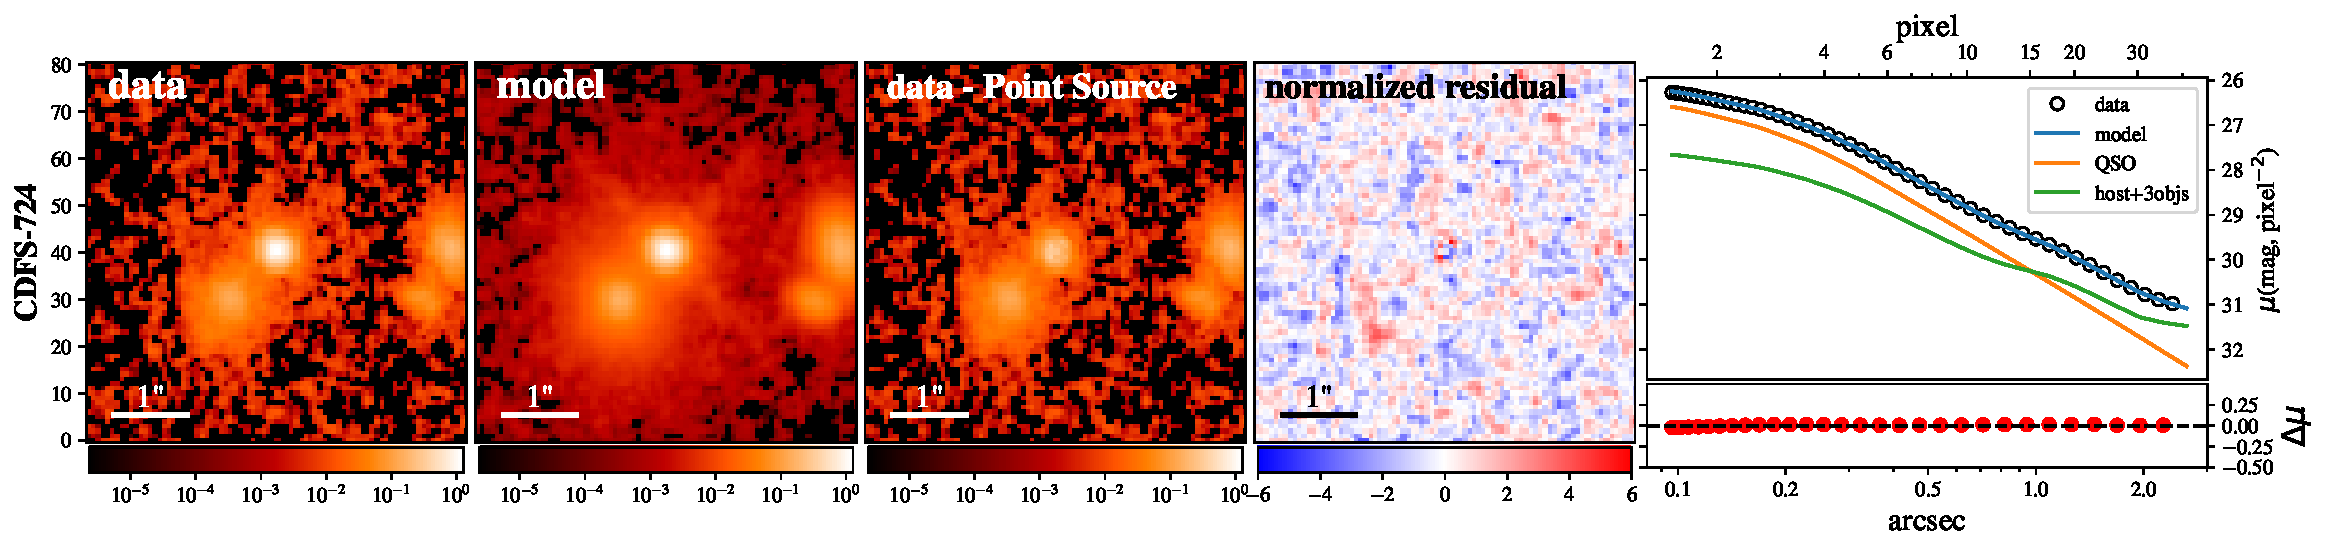
\includegraphics[height=0.25\textwidth]{fig/best_fit_CDFS-724_SB_profile.pdf}
}
\figurenum{1}
\caption{Continued.}
\end{figure*} 

\begin{figure*}
\centering
%\hspace{-5.5em}
{
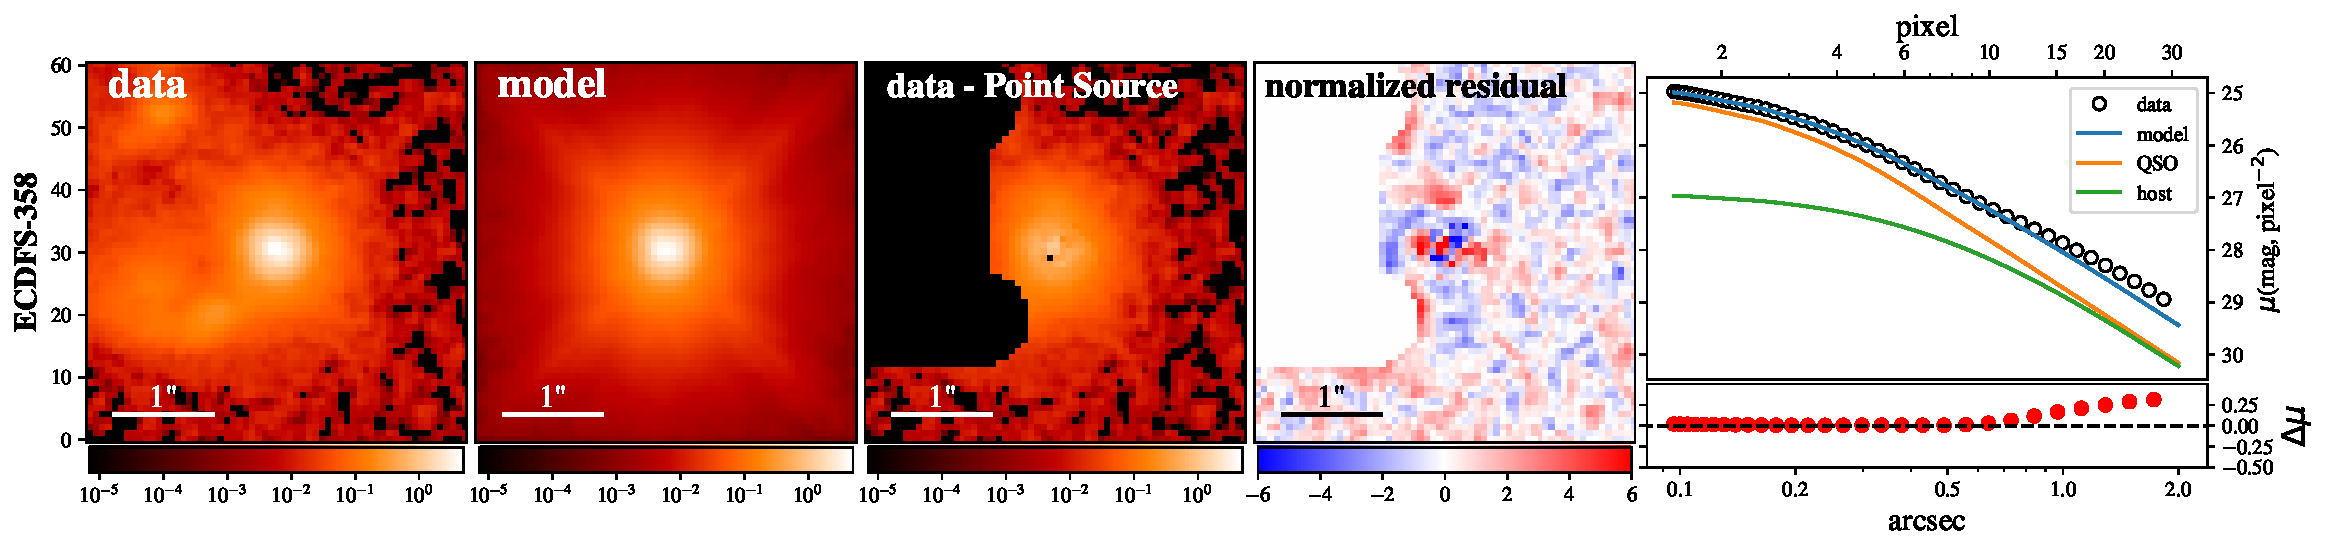
\includegraphics[height=0.25\textwidth]{fig/best_fit_ECDFS-358_SB_profile.pdf}
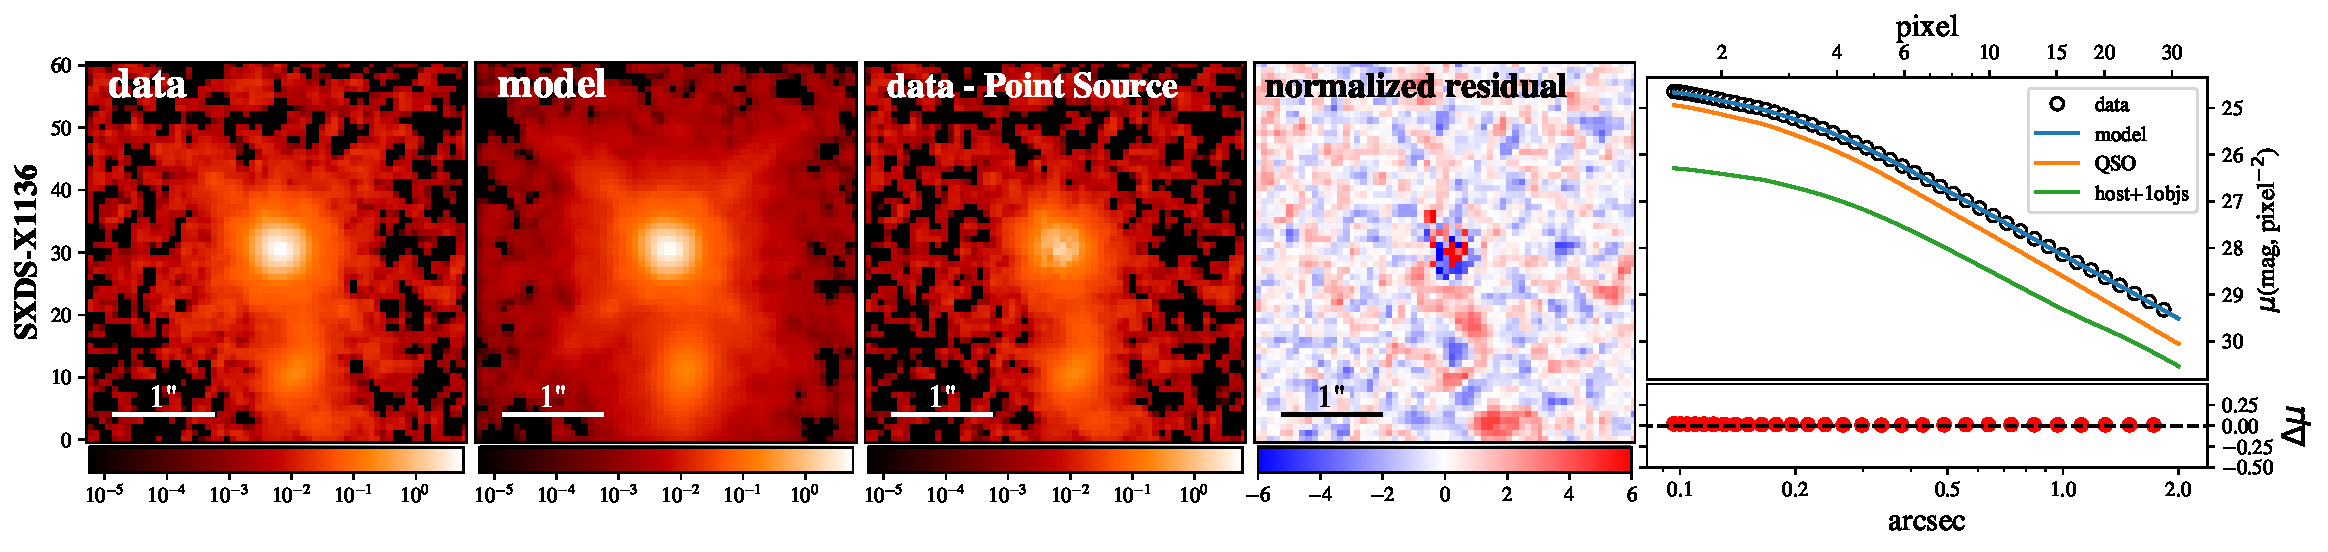
\includegraphics[height=0.25\textwidth]{fig/best_fit_SXDS-X1136_SB_profile.pdf}
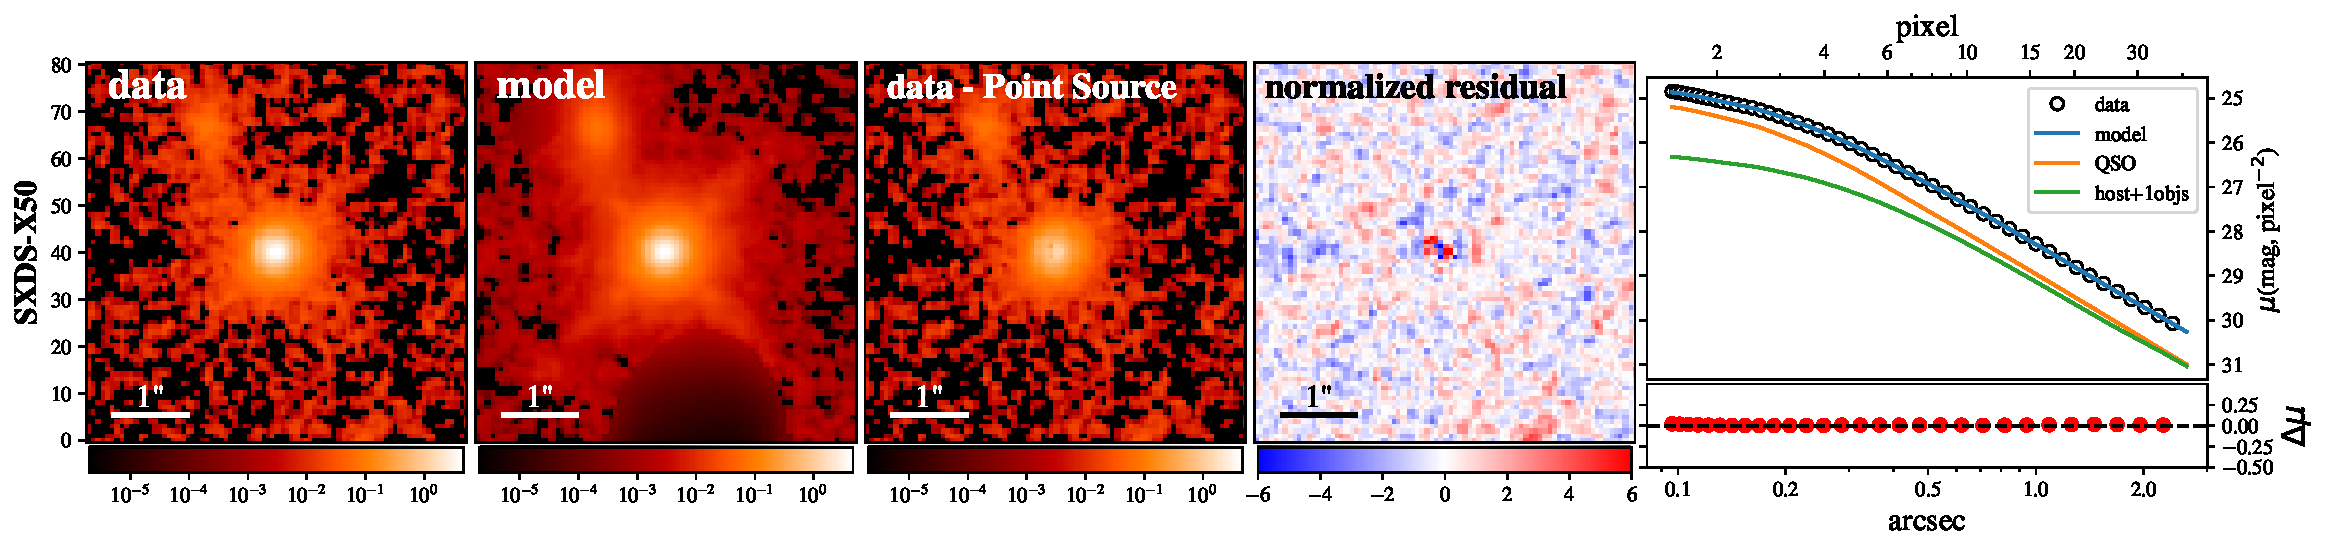
\includegraphics[height=0.25\textwidth]{fig/best_fit_SXDS-X50_SB_profile.pdf}
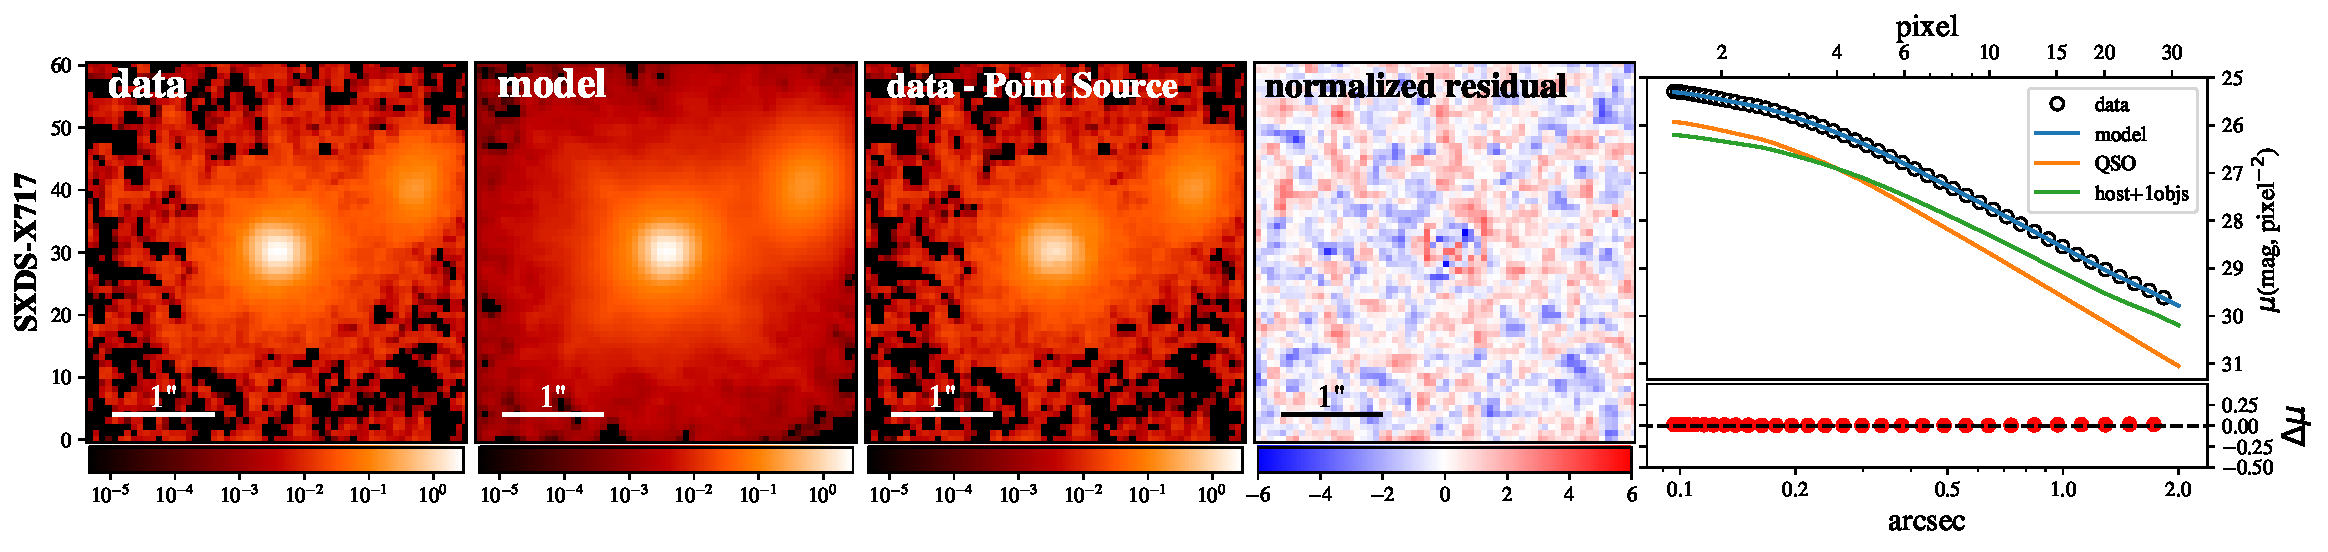
\includegraphics[height=0.25\textwidth]{fig/best_fit_SXDS-X717_SB_profile.pdf}
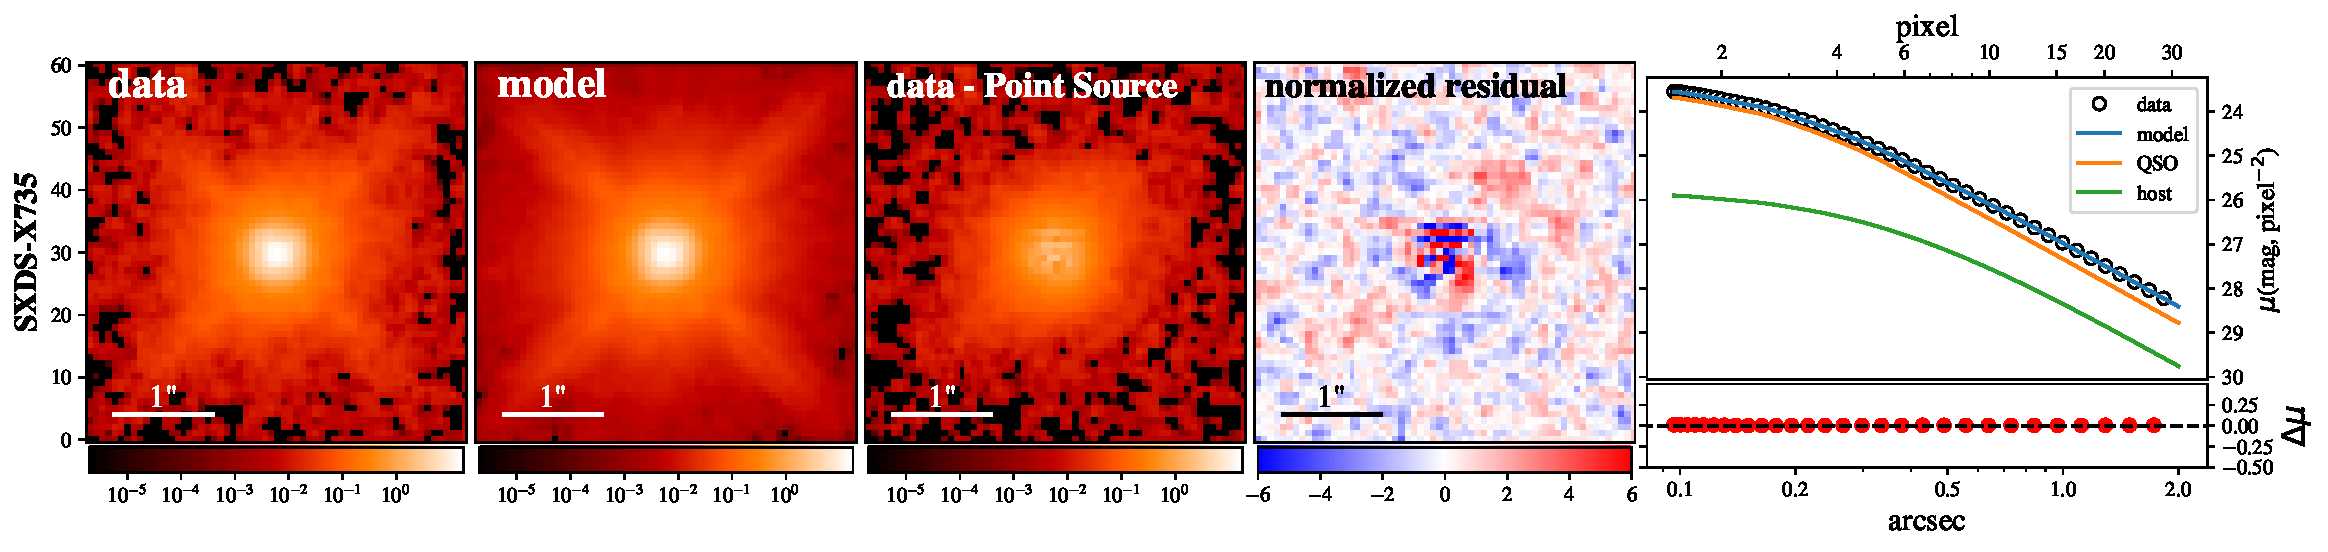
\includegraphics[height=0.25\textwidth]{fig/best_fit_SXDS-X735_SB_profile.pdf}
}
\figurenum{1}
\caption{Continued.}
\end{figure*} 

\begin{figure*}
\centering
%\hspace{-5.5em}
{
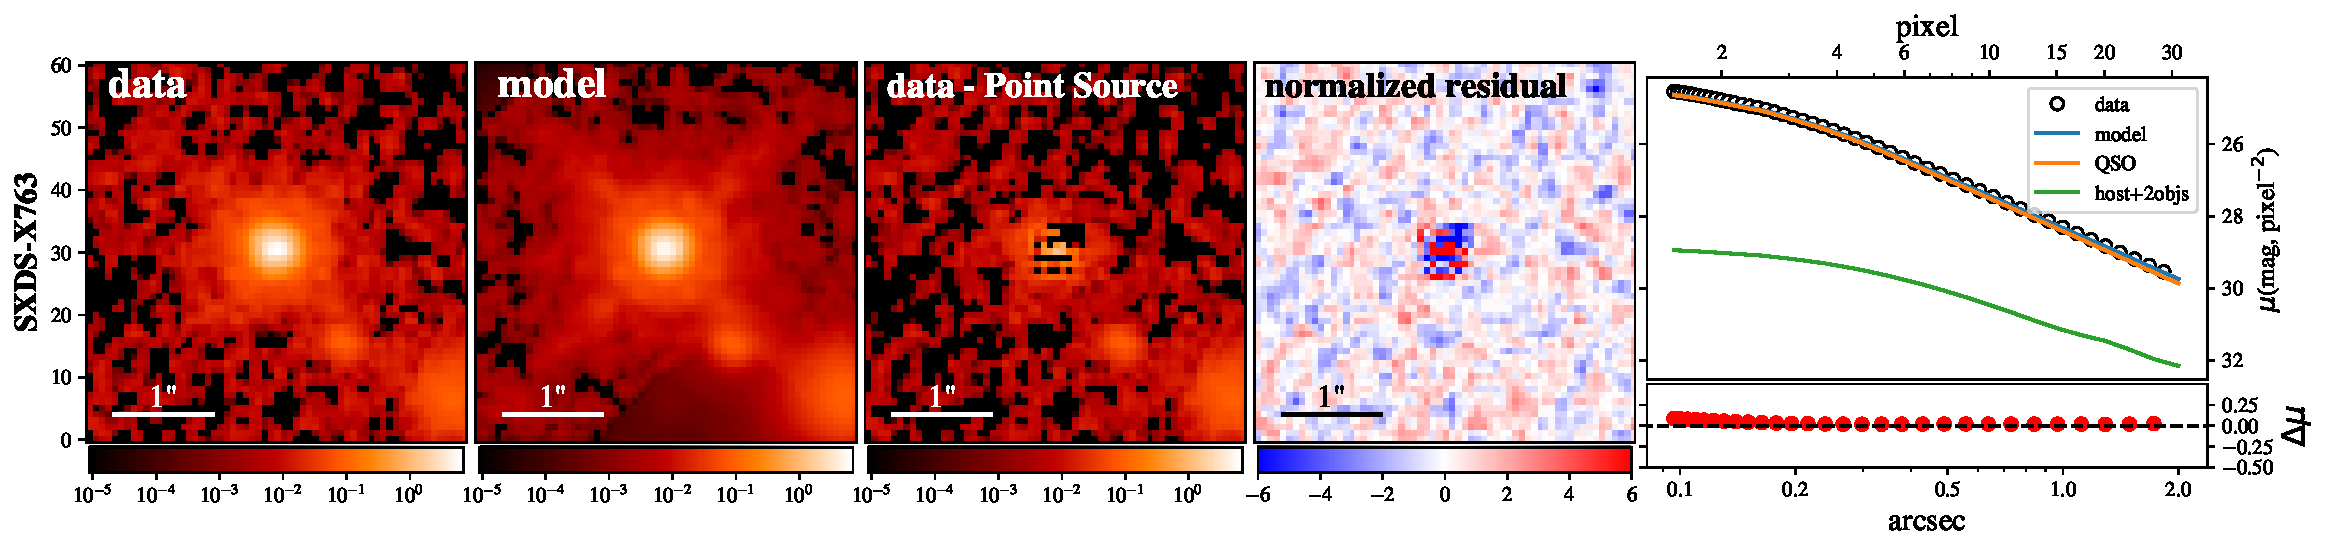
\includegraphics[height=0.25\textwidth]{fig/best_fit_SXDS-X763_SB_profile.pdf}
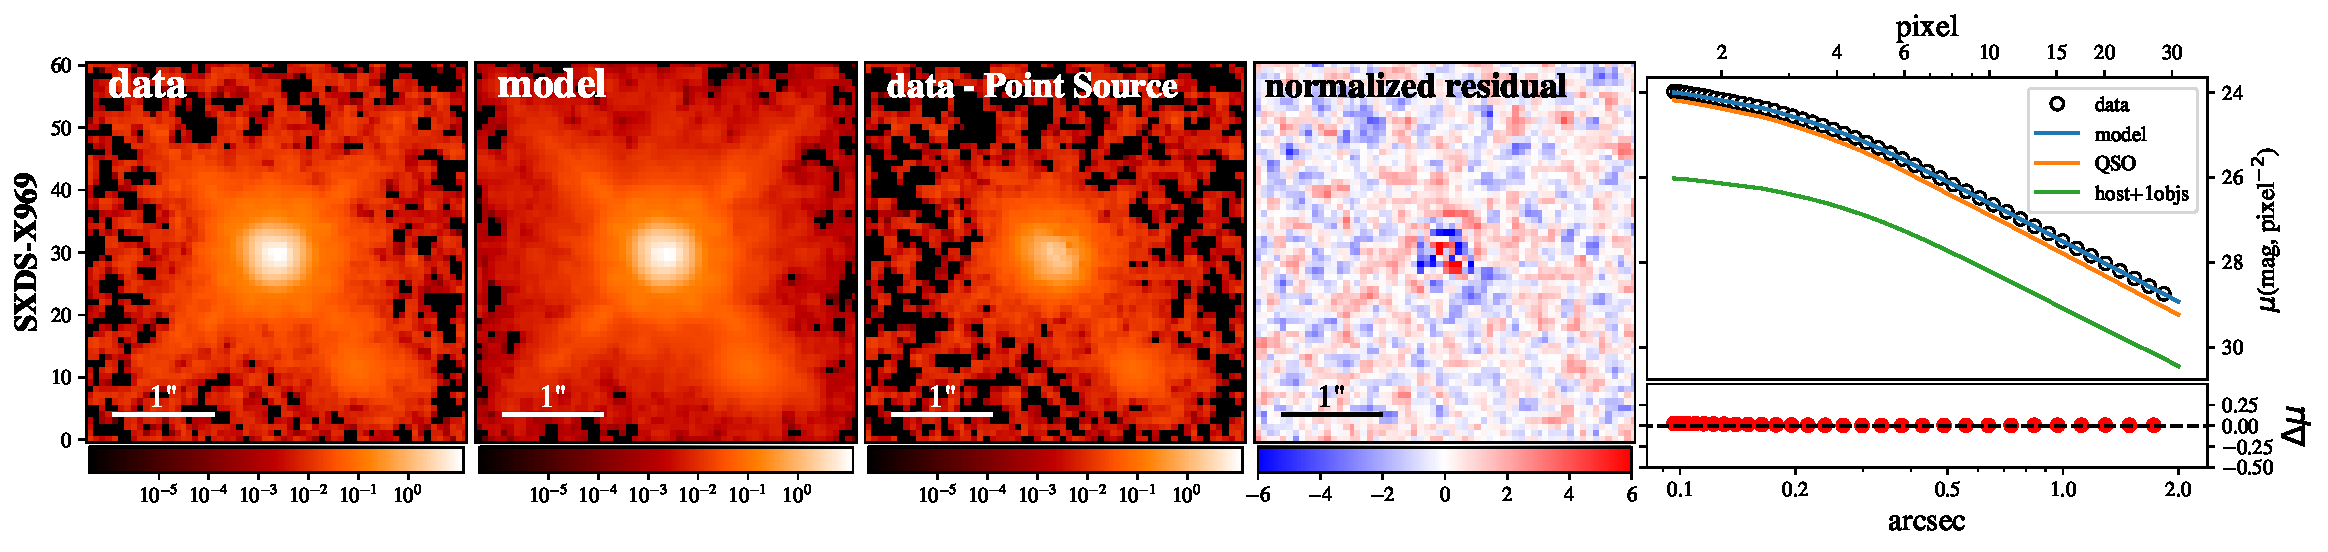
\includegraphics[height=0.25\textwidth]{fig/best_fit_SXDS-X969_SB_profile.pdf}
}
\figurenum{1}
\caption{Continued.}
\end{figure*} 

\begin{figure*}
\centering
{
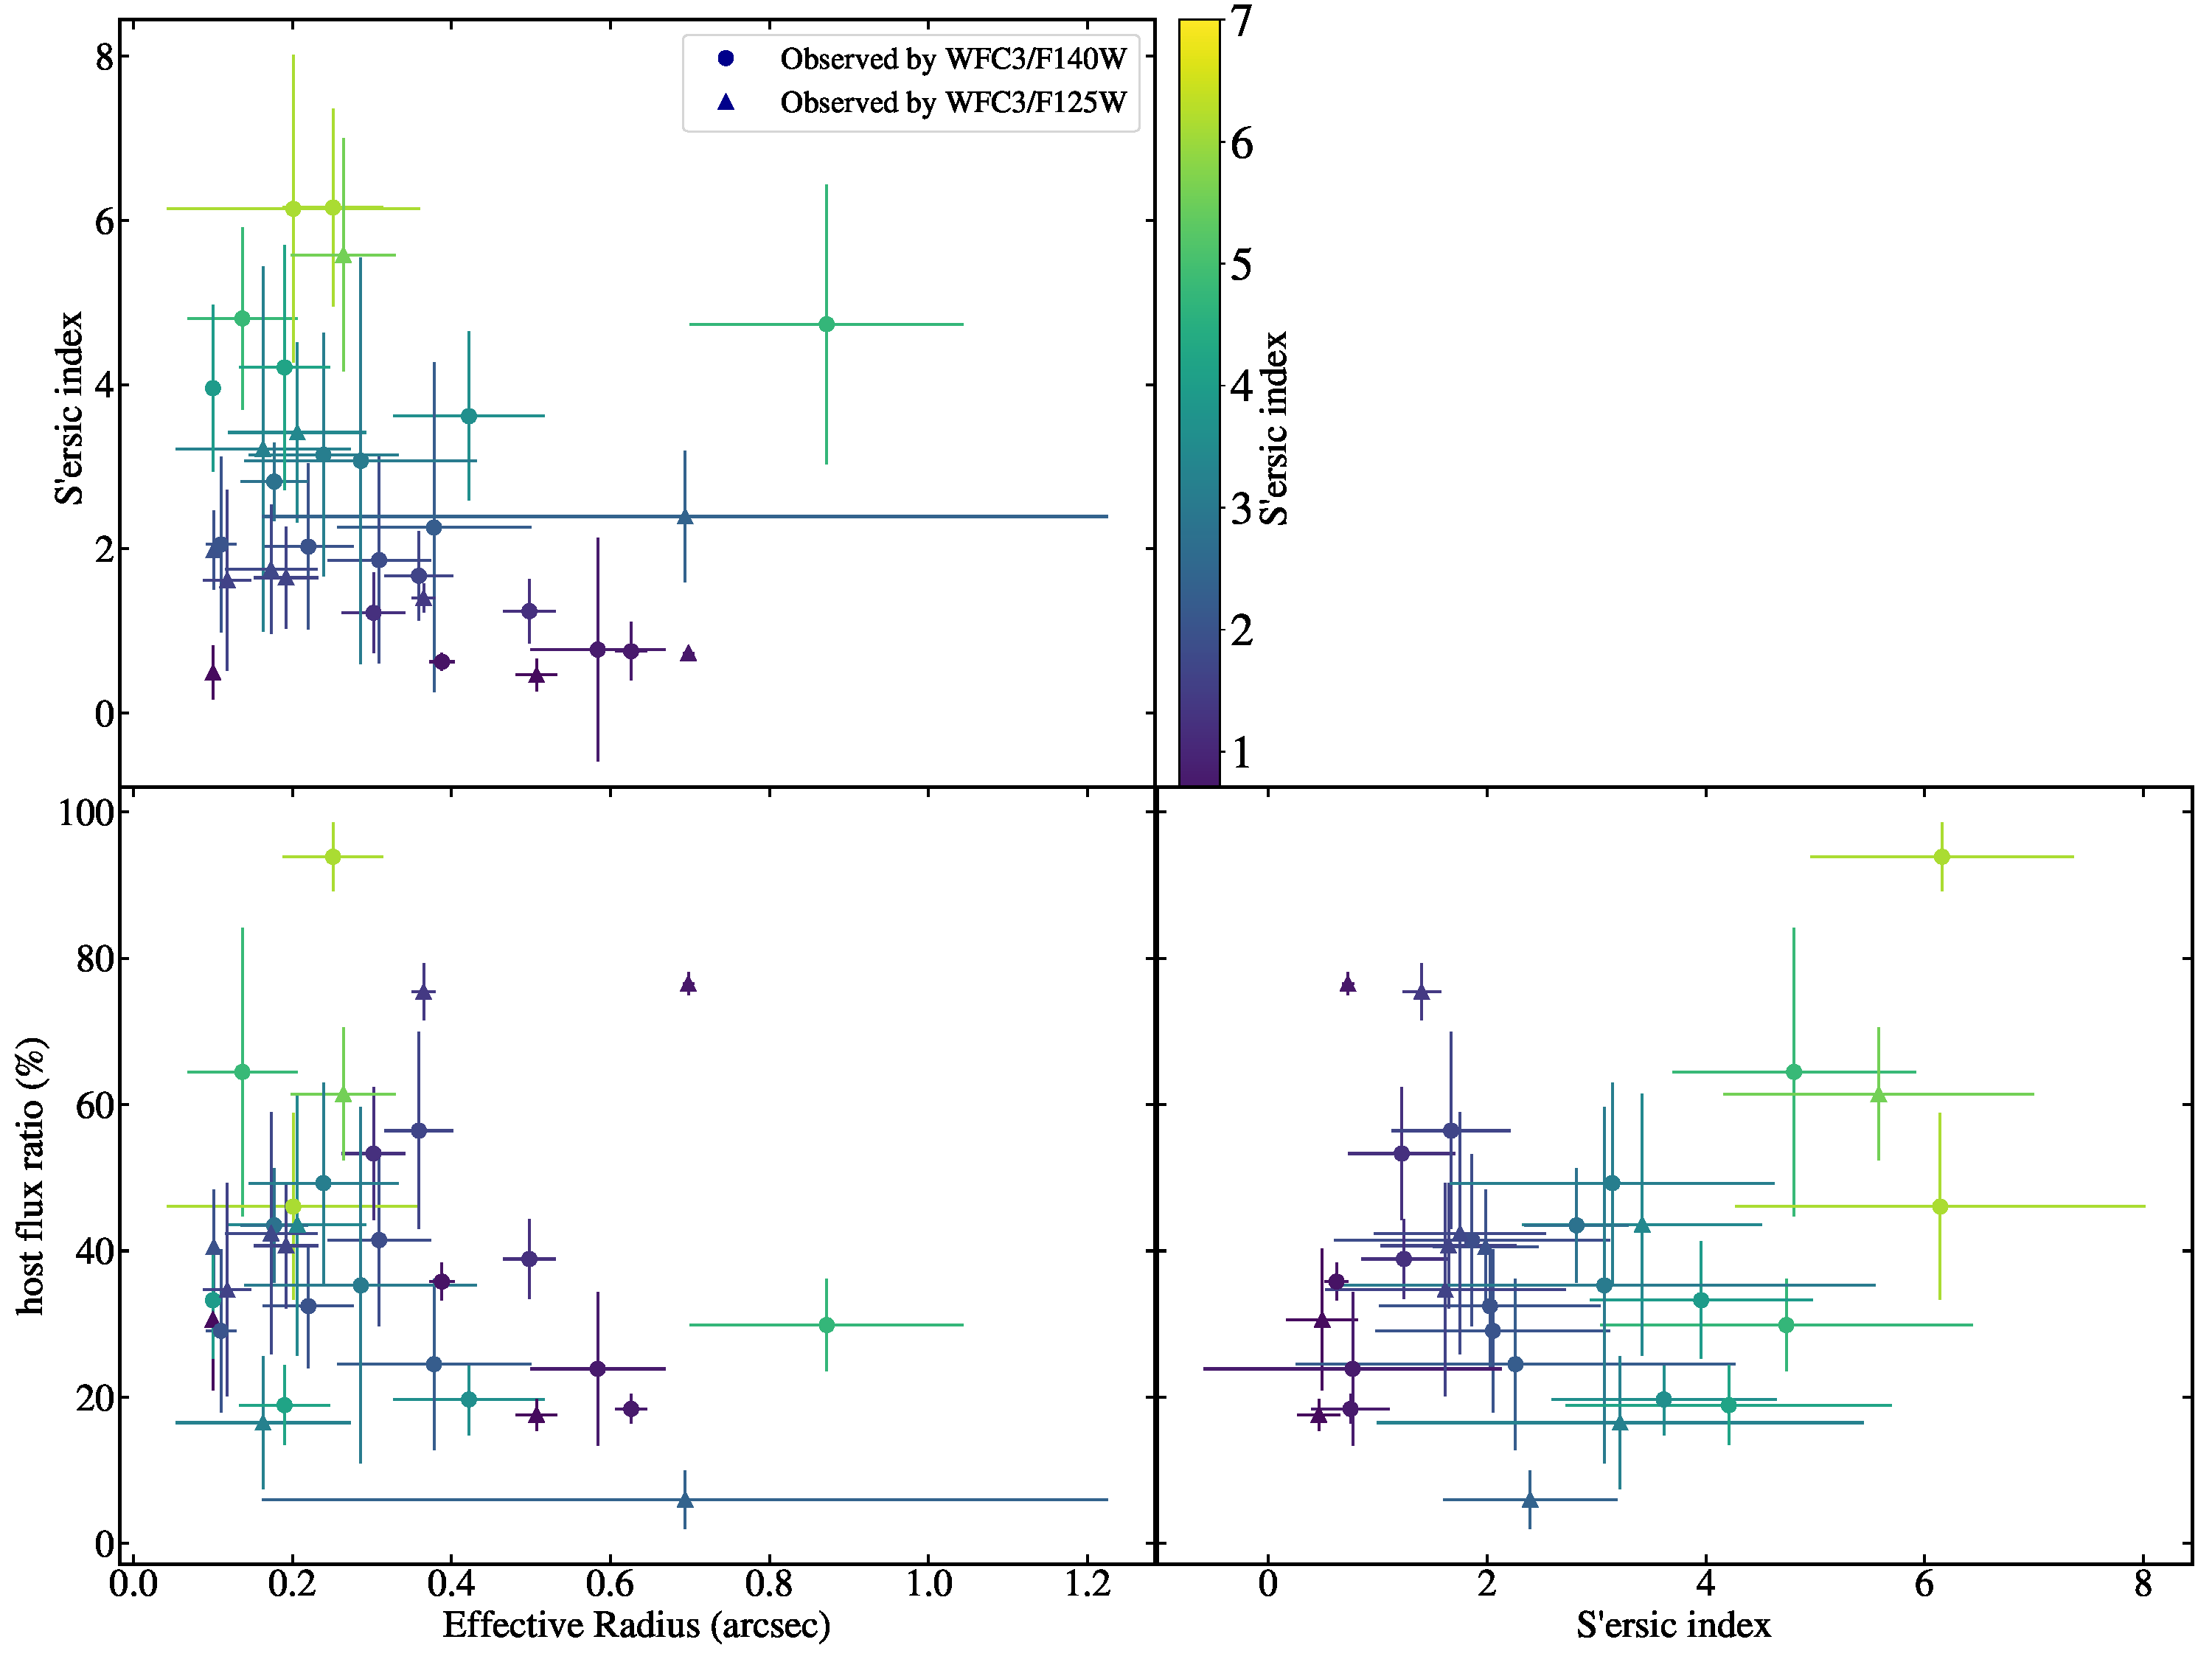
\includegraphics[height=0.75\textwidth]{fig/flux_r_n_corner.pdf}
}
\caption{\label{fig:flux_r_n_corner}
Illustration of the relations between the inferred host \sersic\ parameters.}
\end{figure*} 

\begin{figure*}
\centering
{
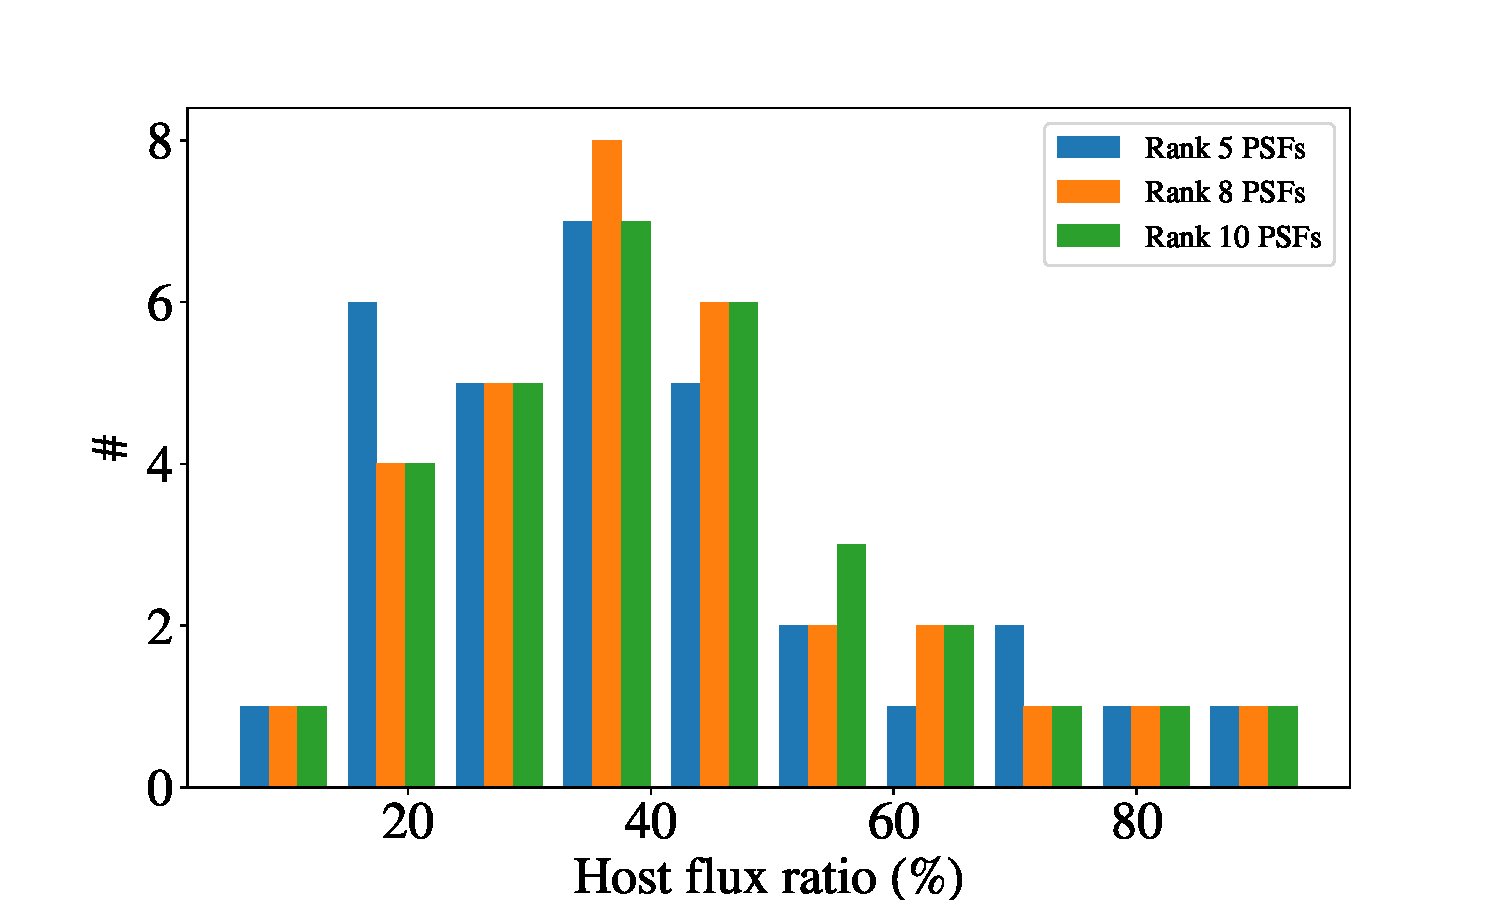
\includegraphics[height=0.35\textwidth]{fig/hist_compare.pdf}
}
\caption{\label{fig:hist_compare} 
Comparison of the histogram of the inferred host flux ratio, based on the different volum of the top-ranked PSFs.}
\end{figure*} 


\begin{figure*}
\centering
\begin{tabular}{c c}
{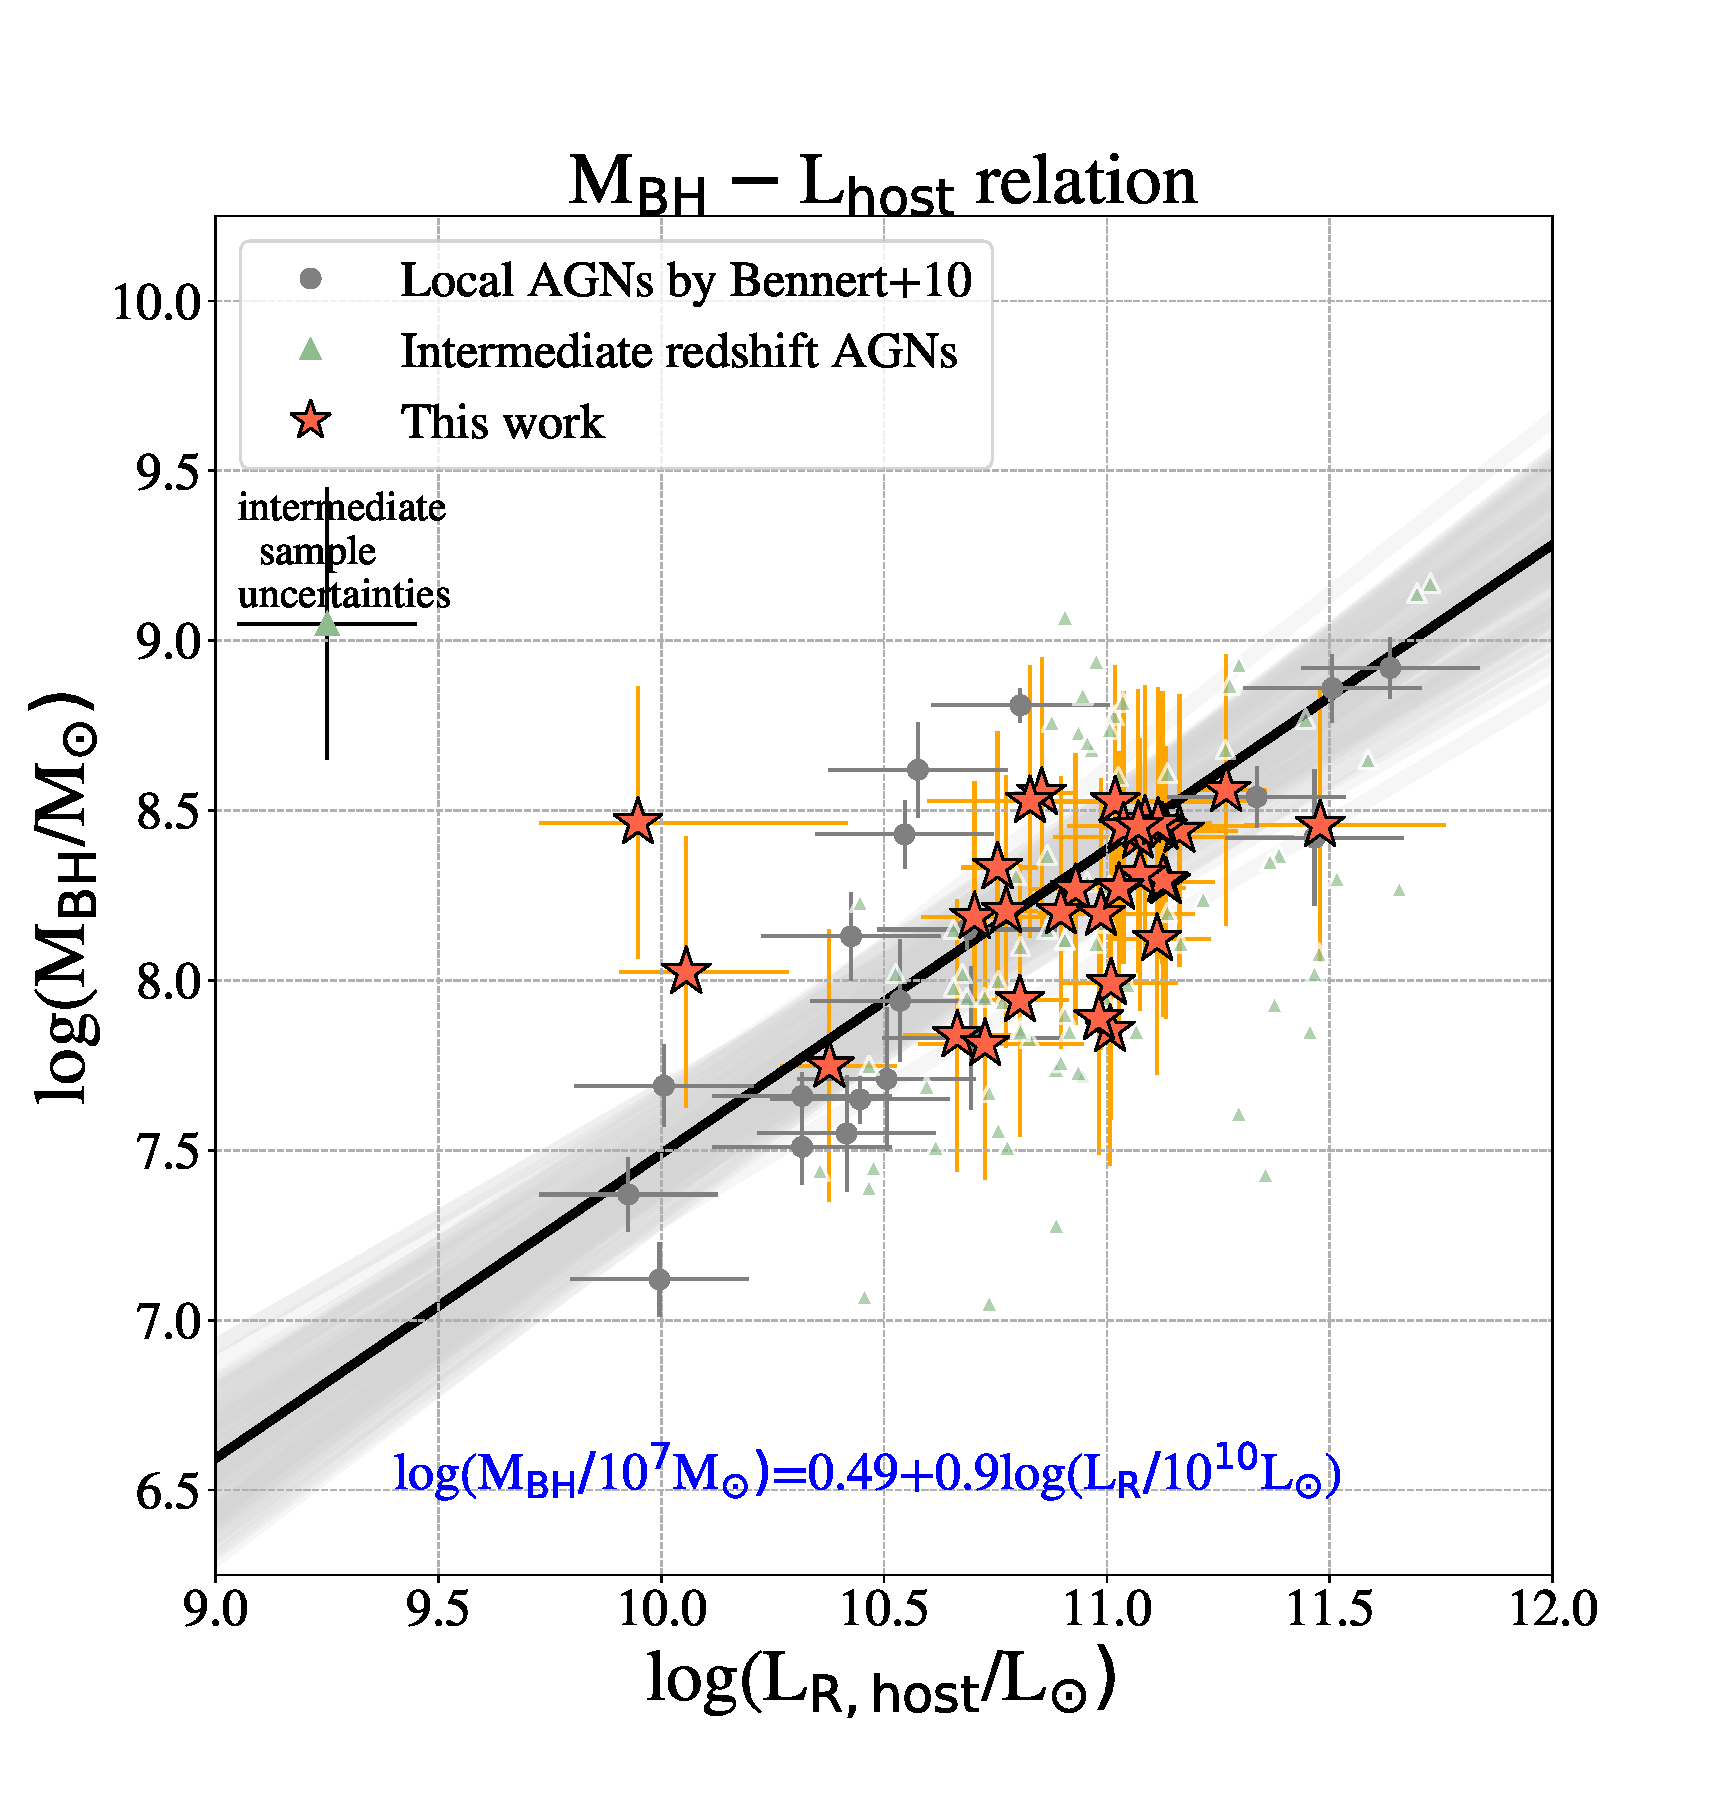
\includegraphics[width=0.5\textwidth]{fig/MBH-L_obs.pdf}}&
{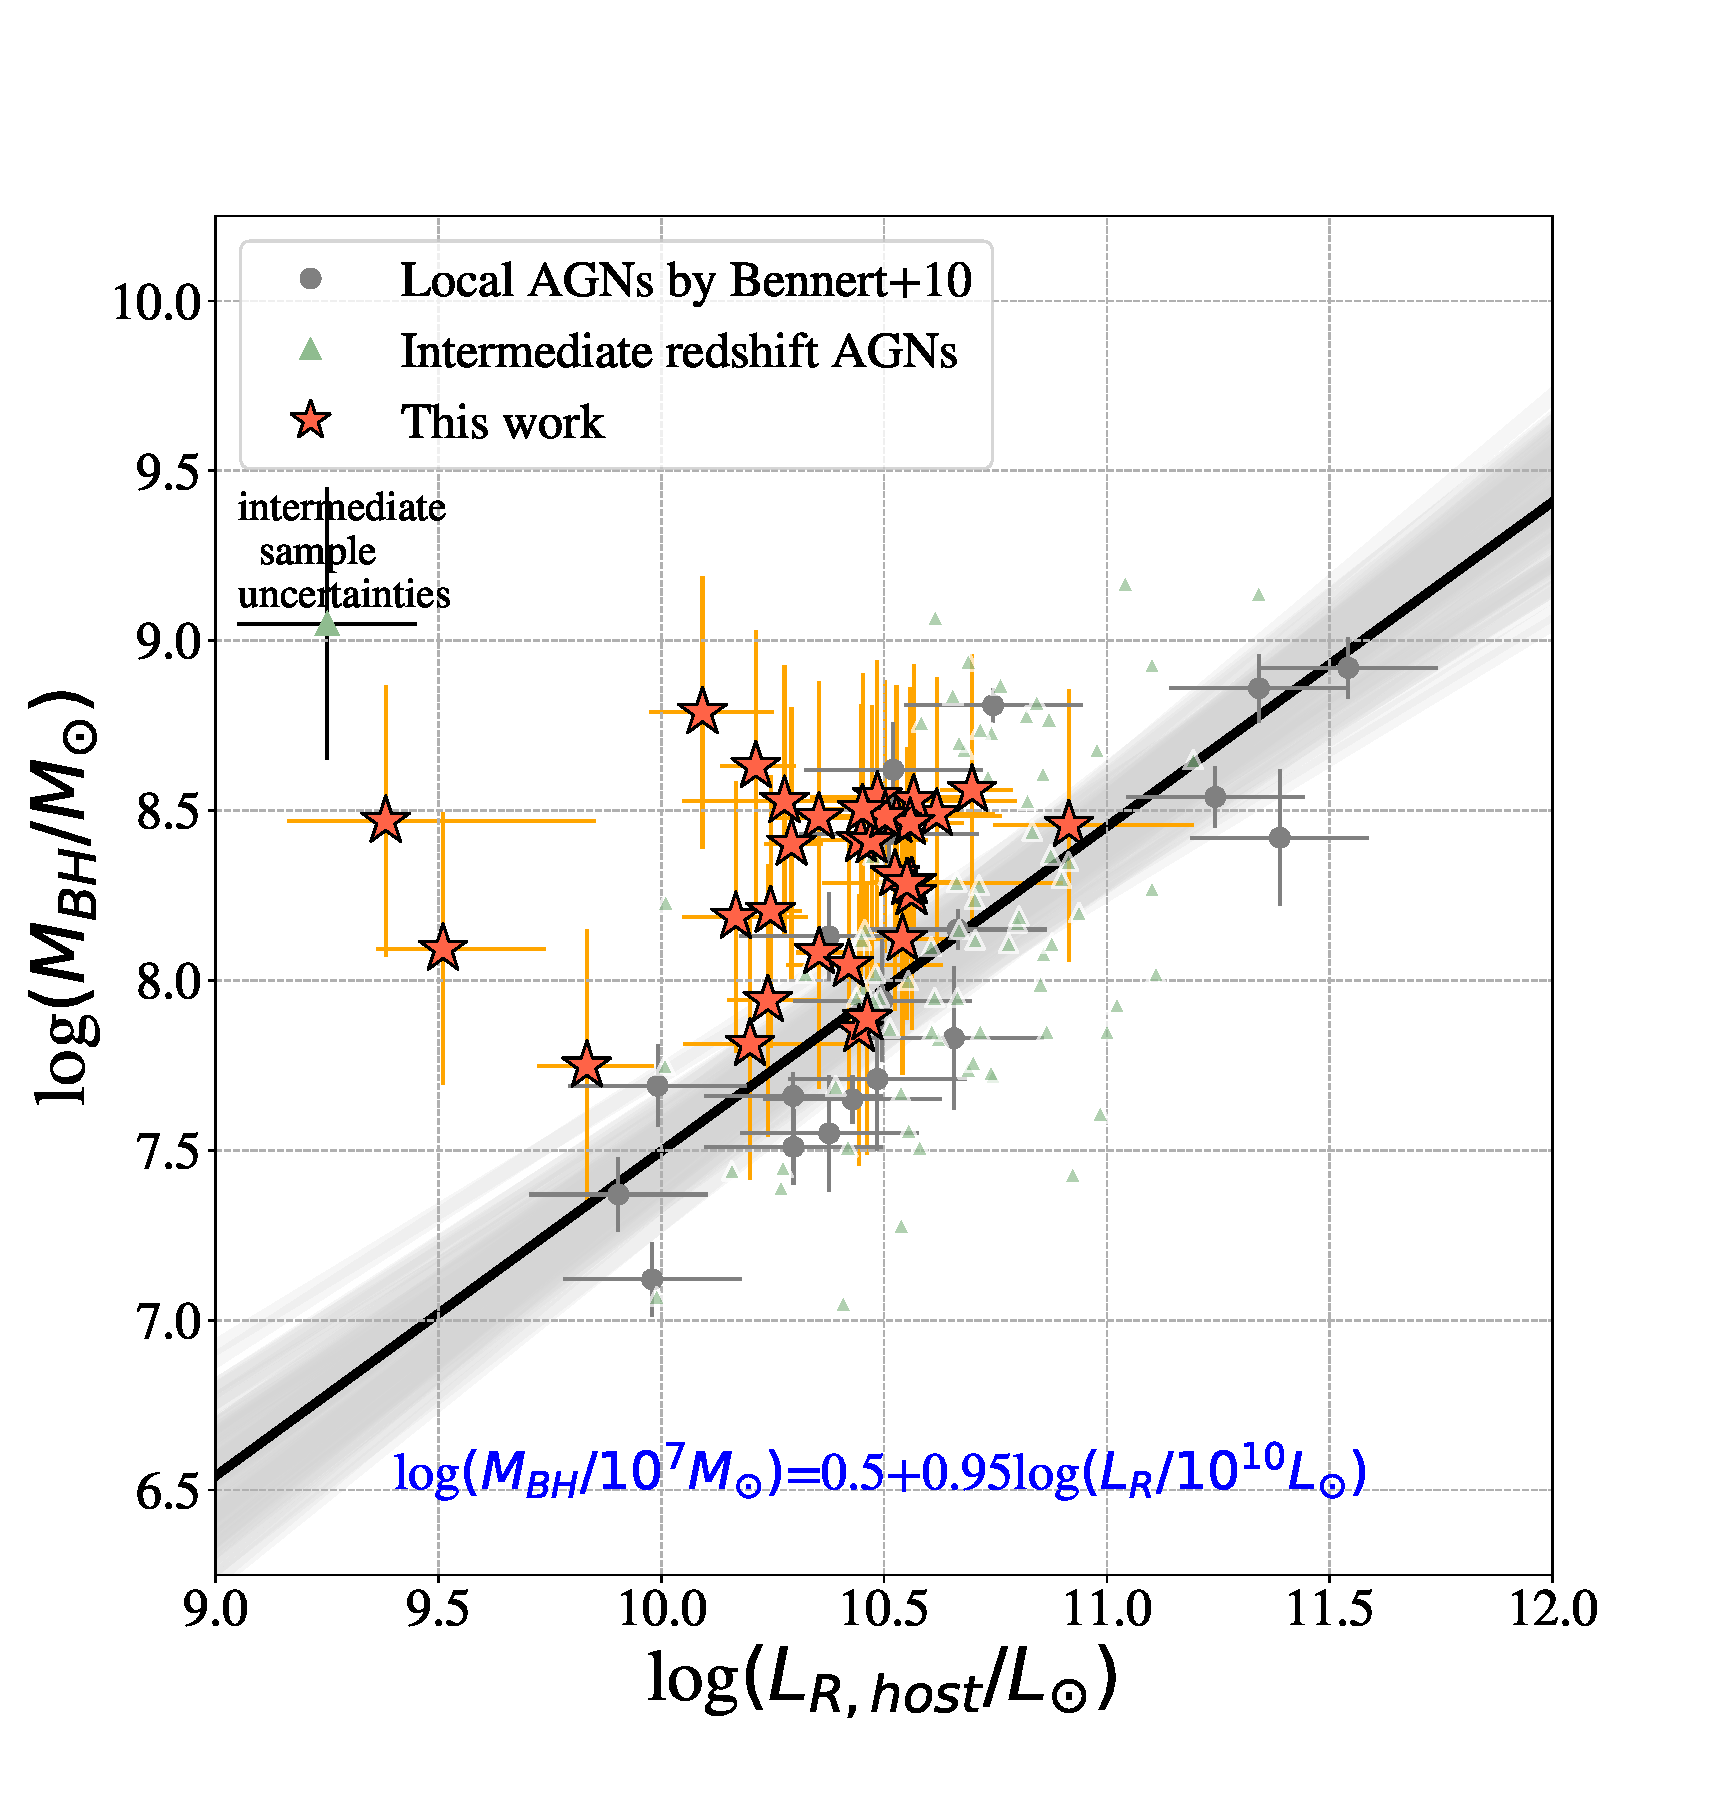
\includegraphics[width=0.5\textwidth]{fig/MBH-L_ev.pdf}}\\
\end{tabular}
\caption{\label{fig:ML} 
Illustration of observed (left) and evolution-corrected (right) correlations between \mbh-\lhost, with local linear relation indicated.  The redshift are color-coded, for distant and intermediate AGNs.
}
\end{figure*} 

\begin{figure}
\centering
{
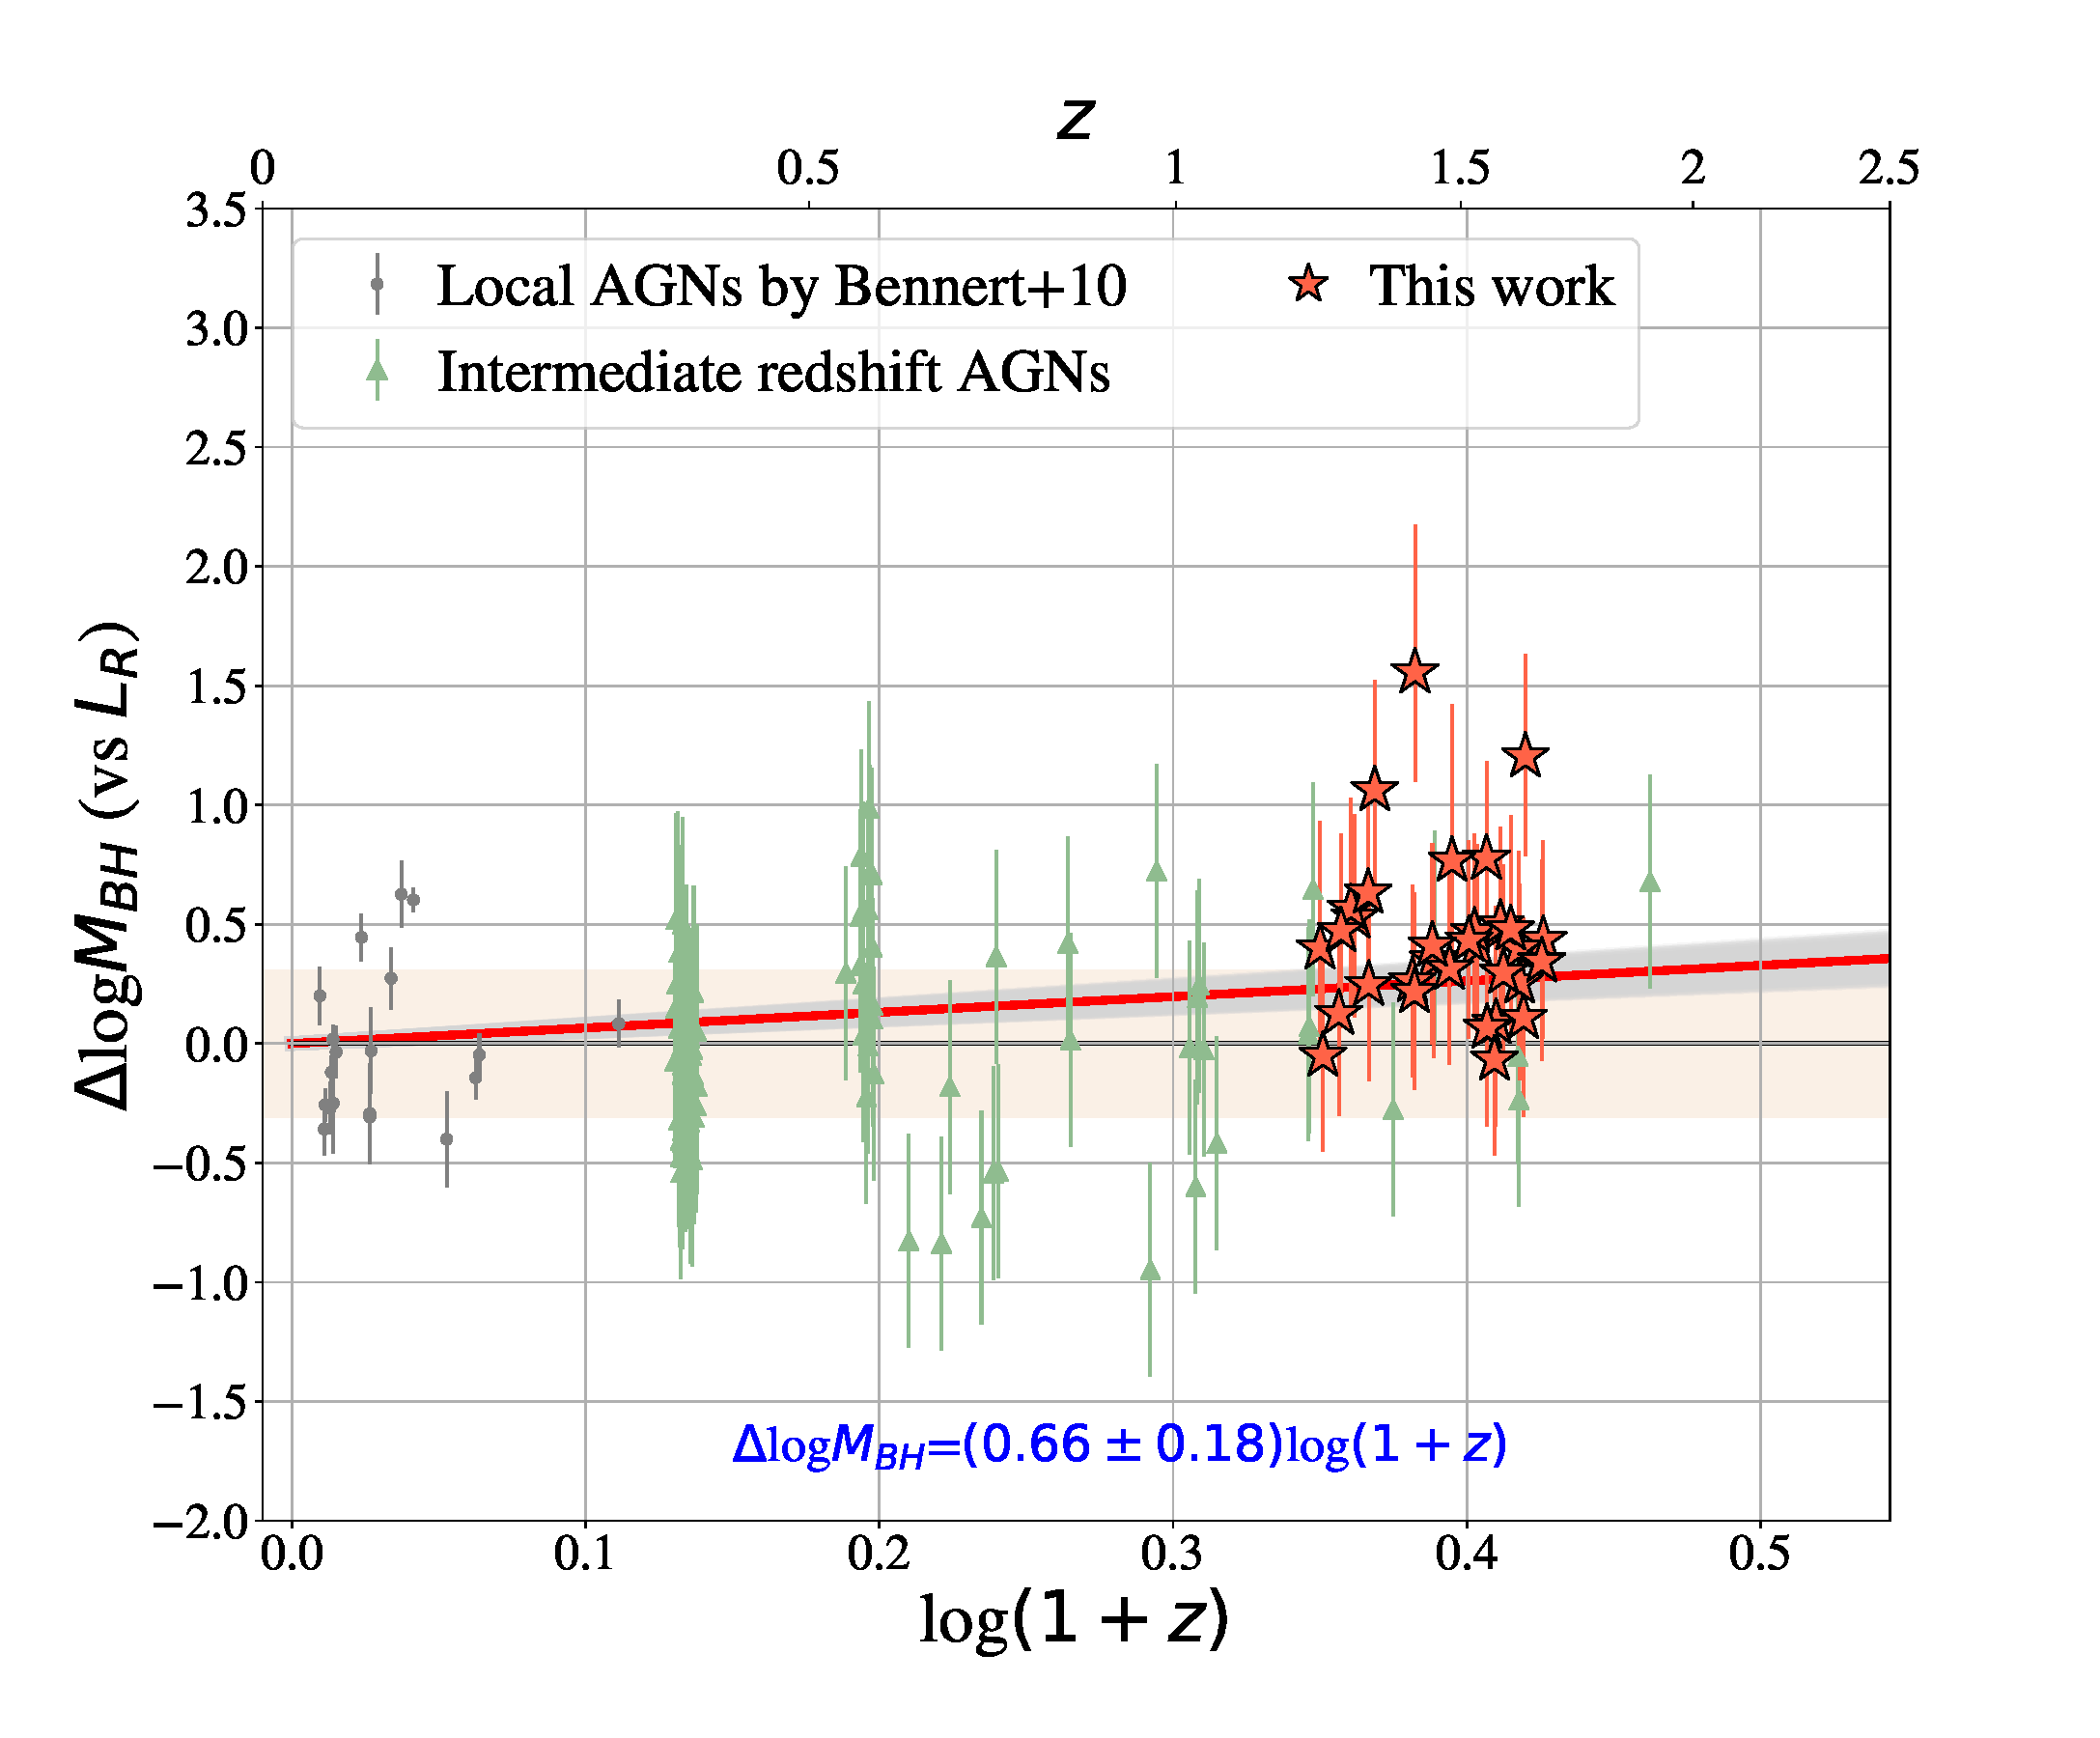
\includegraphics[height=0.4\textwidth]{fig/MBH-L-vz.pdf}
}
\caption{\label{fig:ML-vz} 
Illustration of the offset in log\mbh\ (VS. $L_R$) as a function of redshift. The orange band is the intrinsic scatter of local linear relation.}
\end{figure} 


\begin{figure}
\centering
{
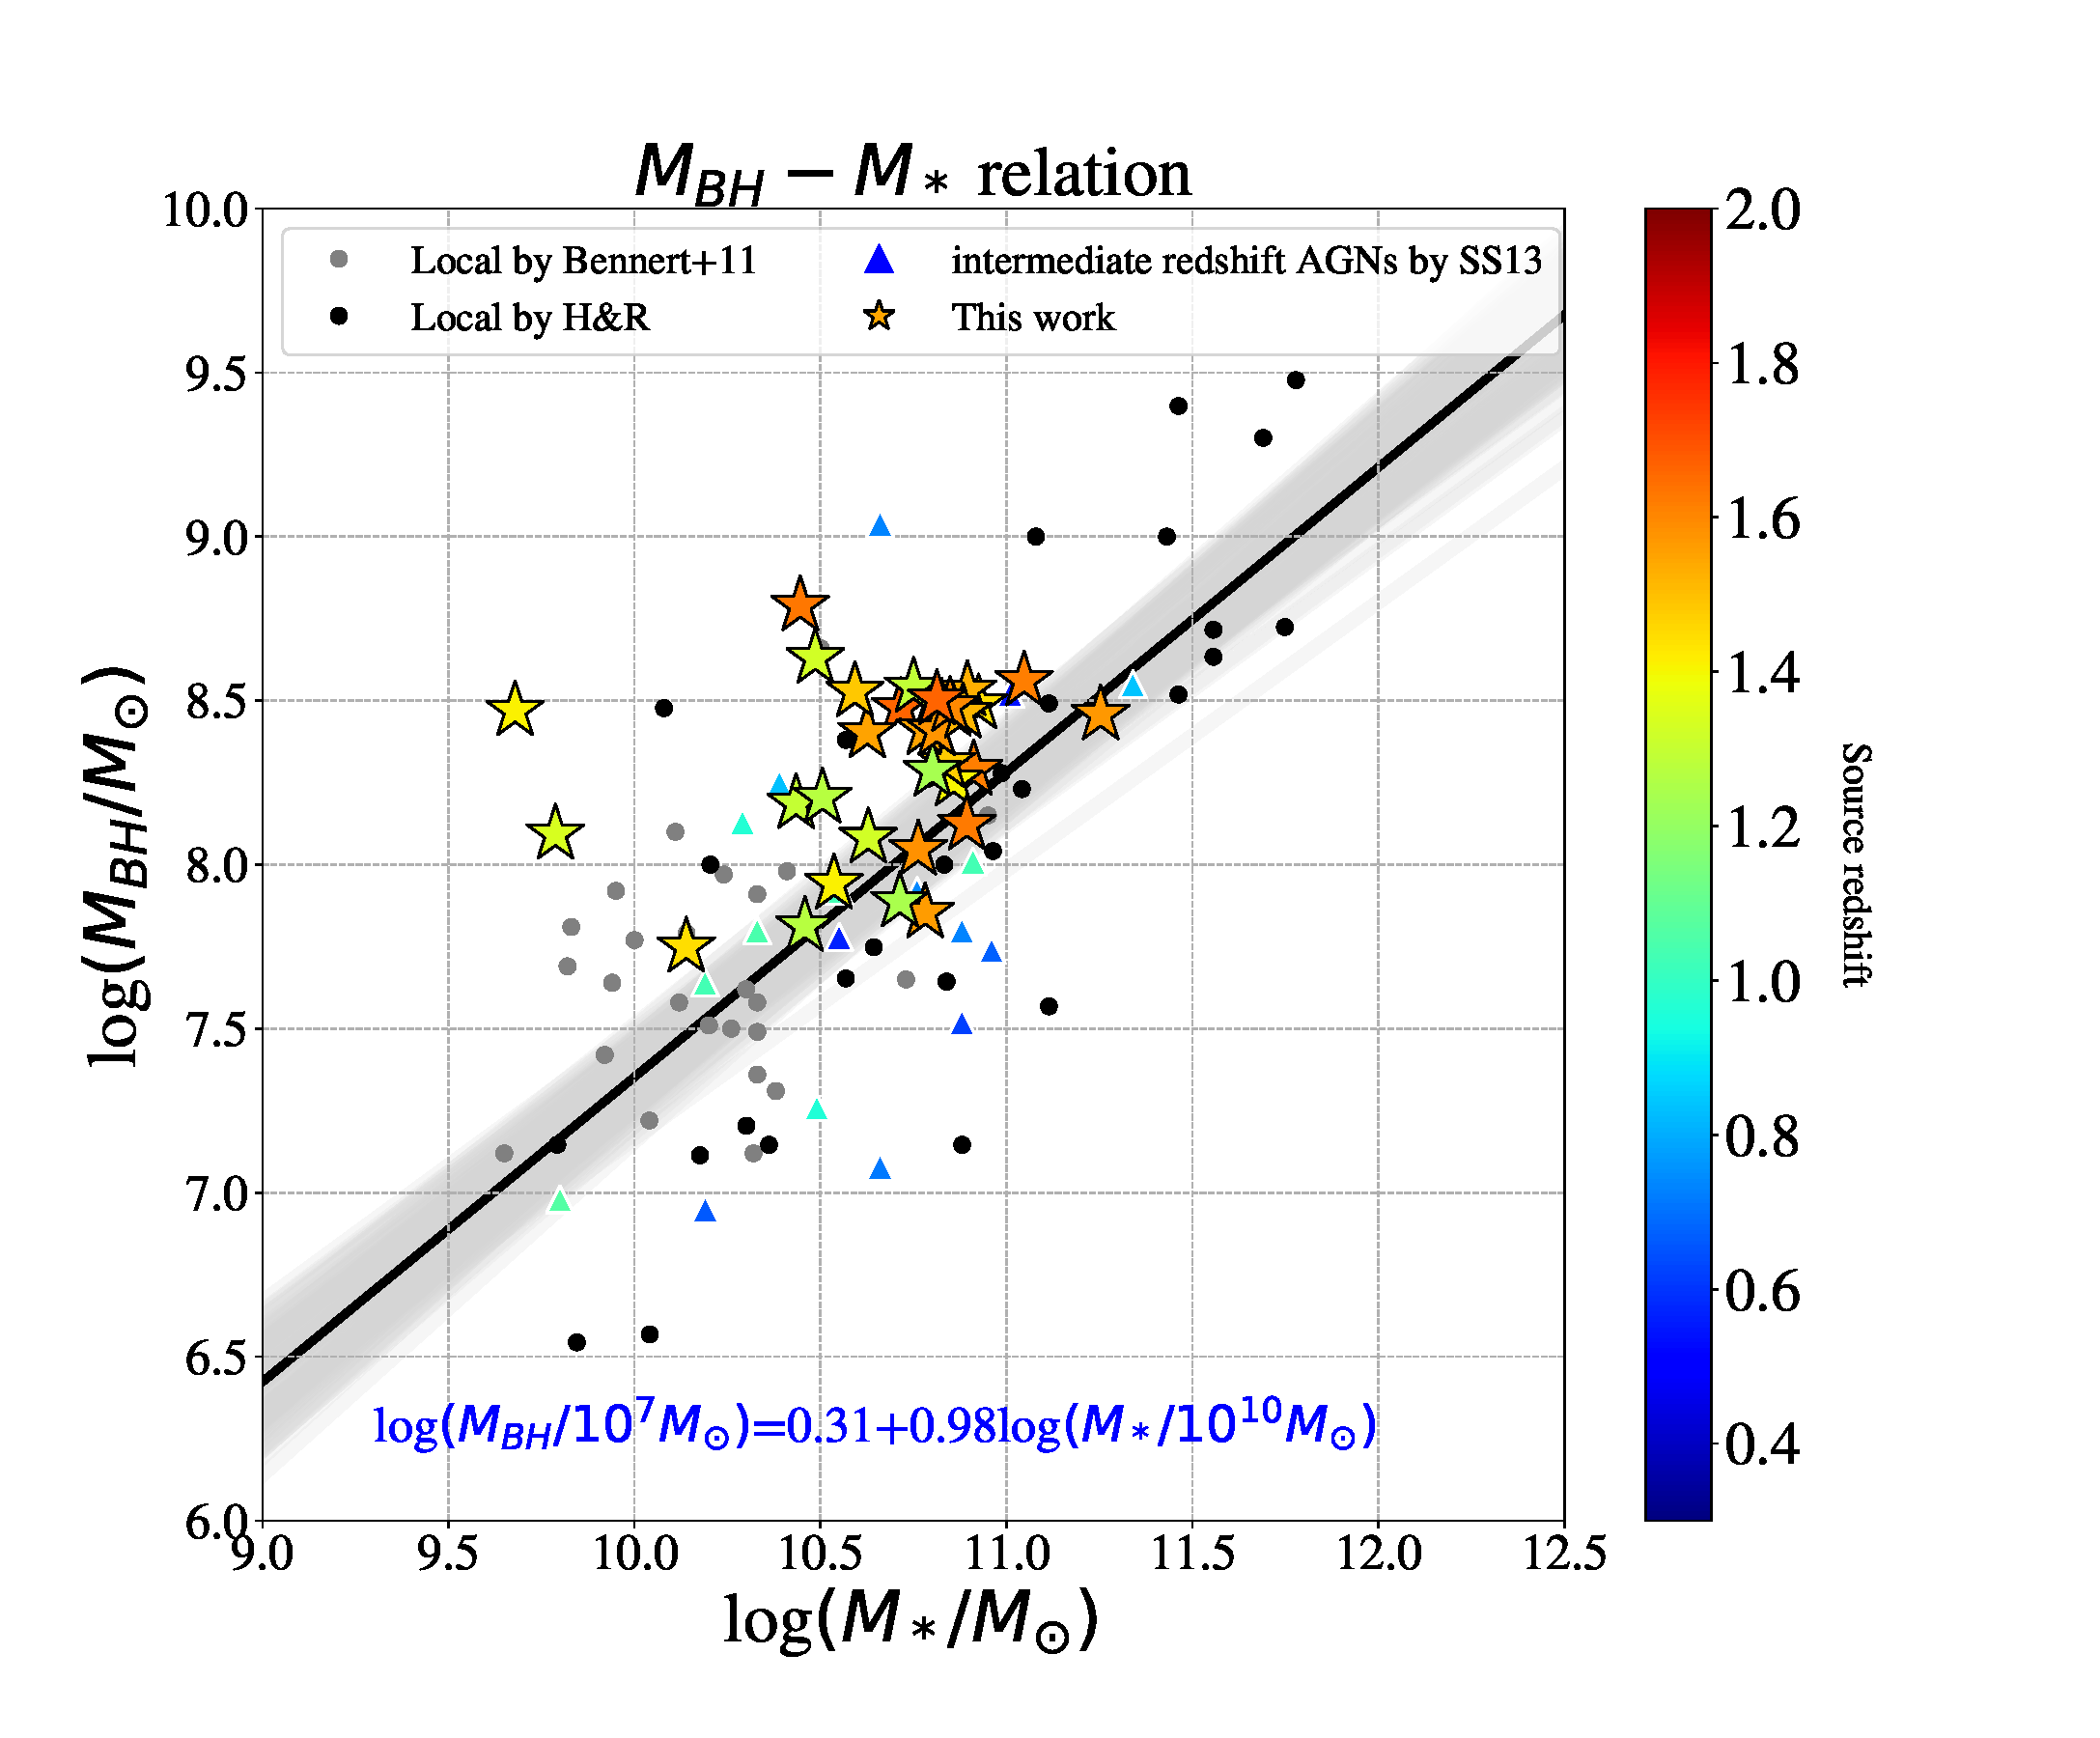
\includegraphics[height=0.4\textwidth]{fig/MBH-Mstar.pdf}
}
\caption{\label{fig:MM} 
Similar to the Figure~\ref{fig:ML}, but the comparison of the \mbh-\smass\ relations.}
\end{figure} 

\begin{figure*}
\centering
\begin{tabular}{c c}
{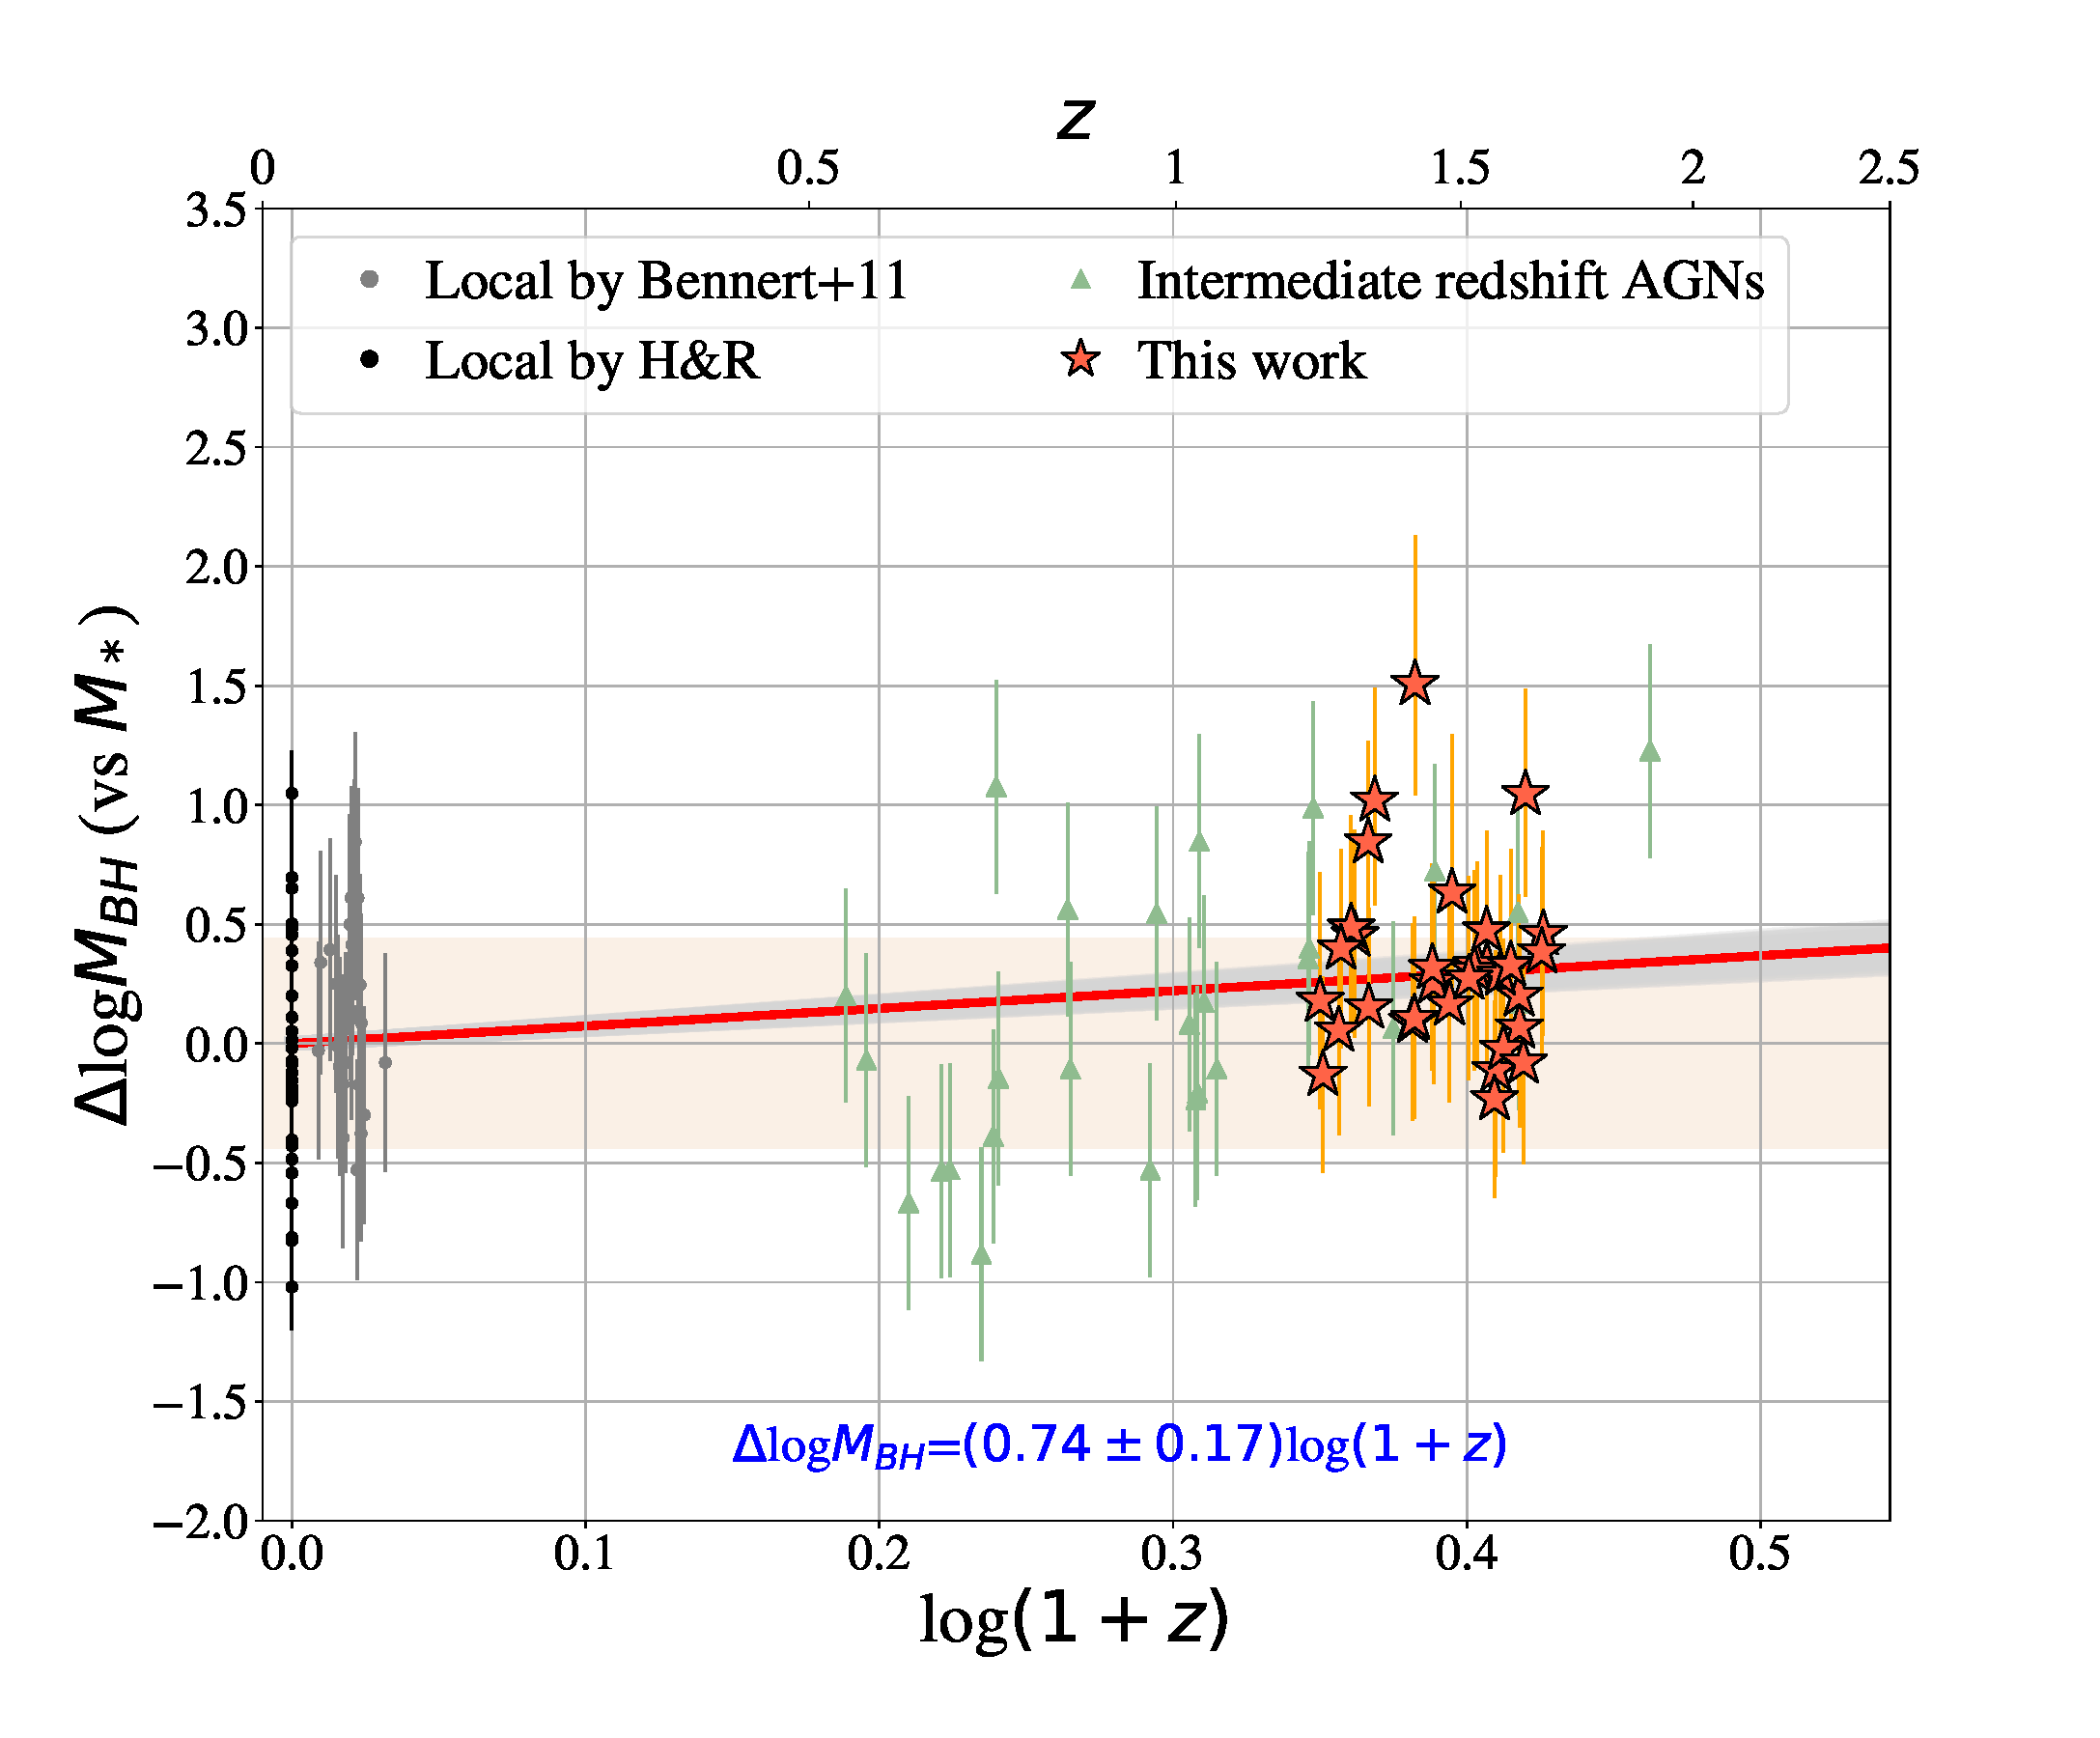
\includegraphics[width=0.5\textwidth]{fig/MBH-Mstar-vz_style1.pdf}}&
{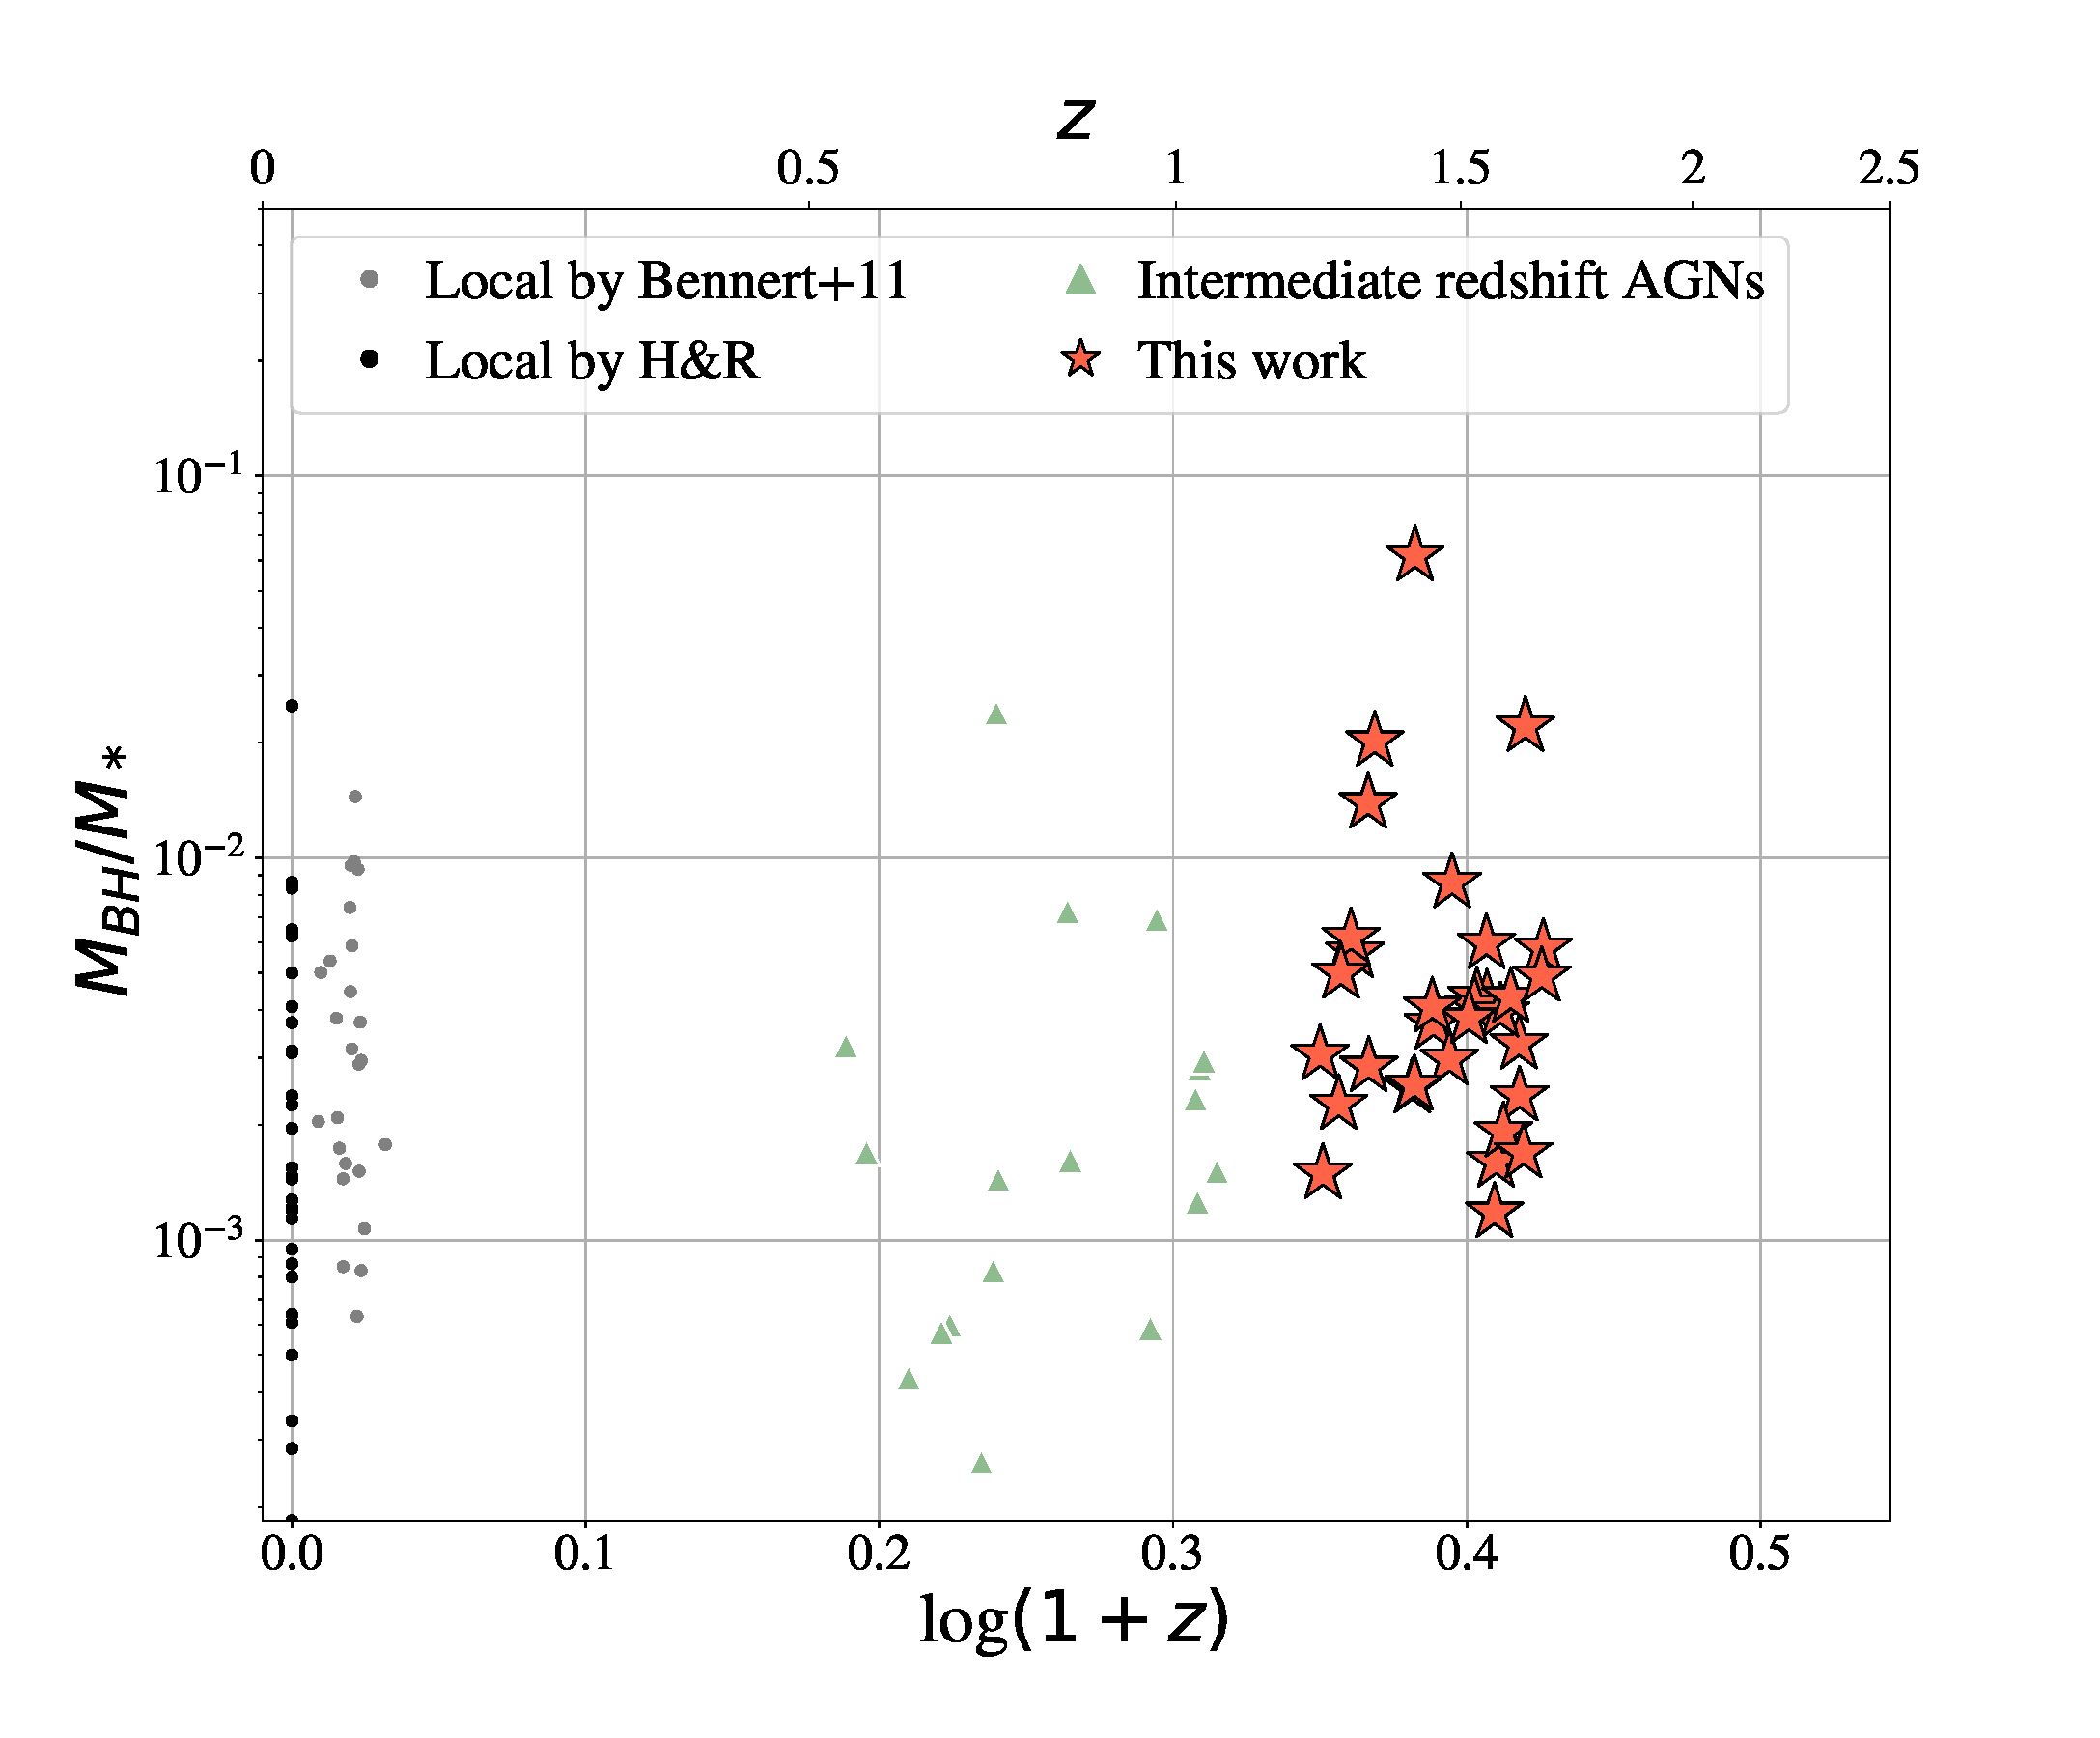
\includegraphics[width=0.5\textwidth]{fig/MBH-Mstar-vz_style0.pdf}}\\
\end{tabular}
\caption{\label{fig:MM-vz} 
Left: illustration of the offset in log\mbh\ (VS. \smass) as a function of redshift. Right: redshift evolution of the \mbh/\smass.  }
\end{figure*} 

\begin{figure*}
\centering
\begin{tabular}{c c}
 \hspace{-2.5em}
{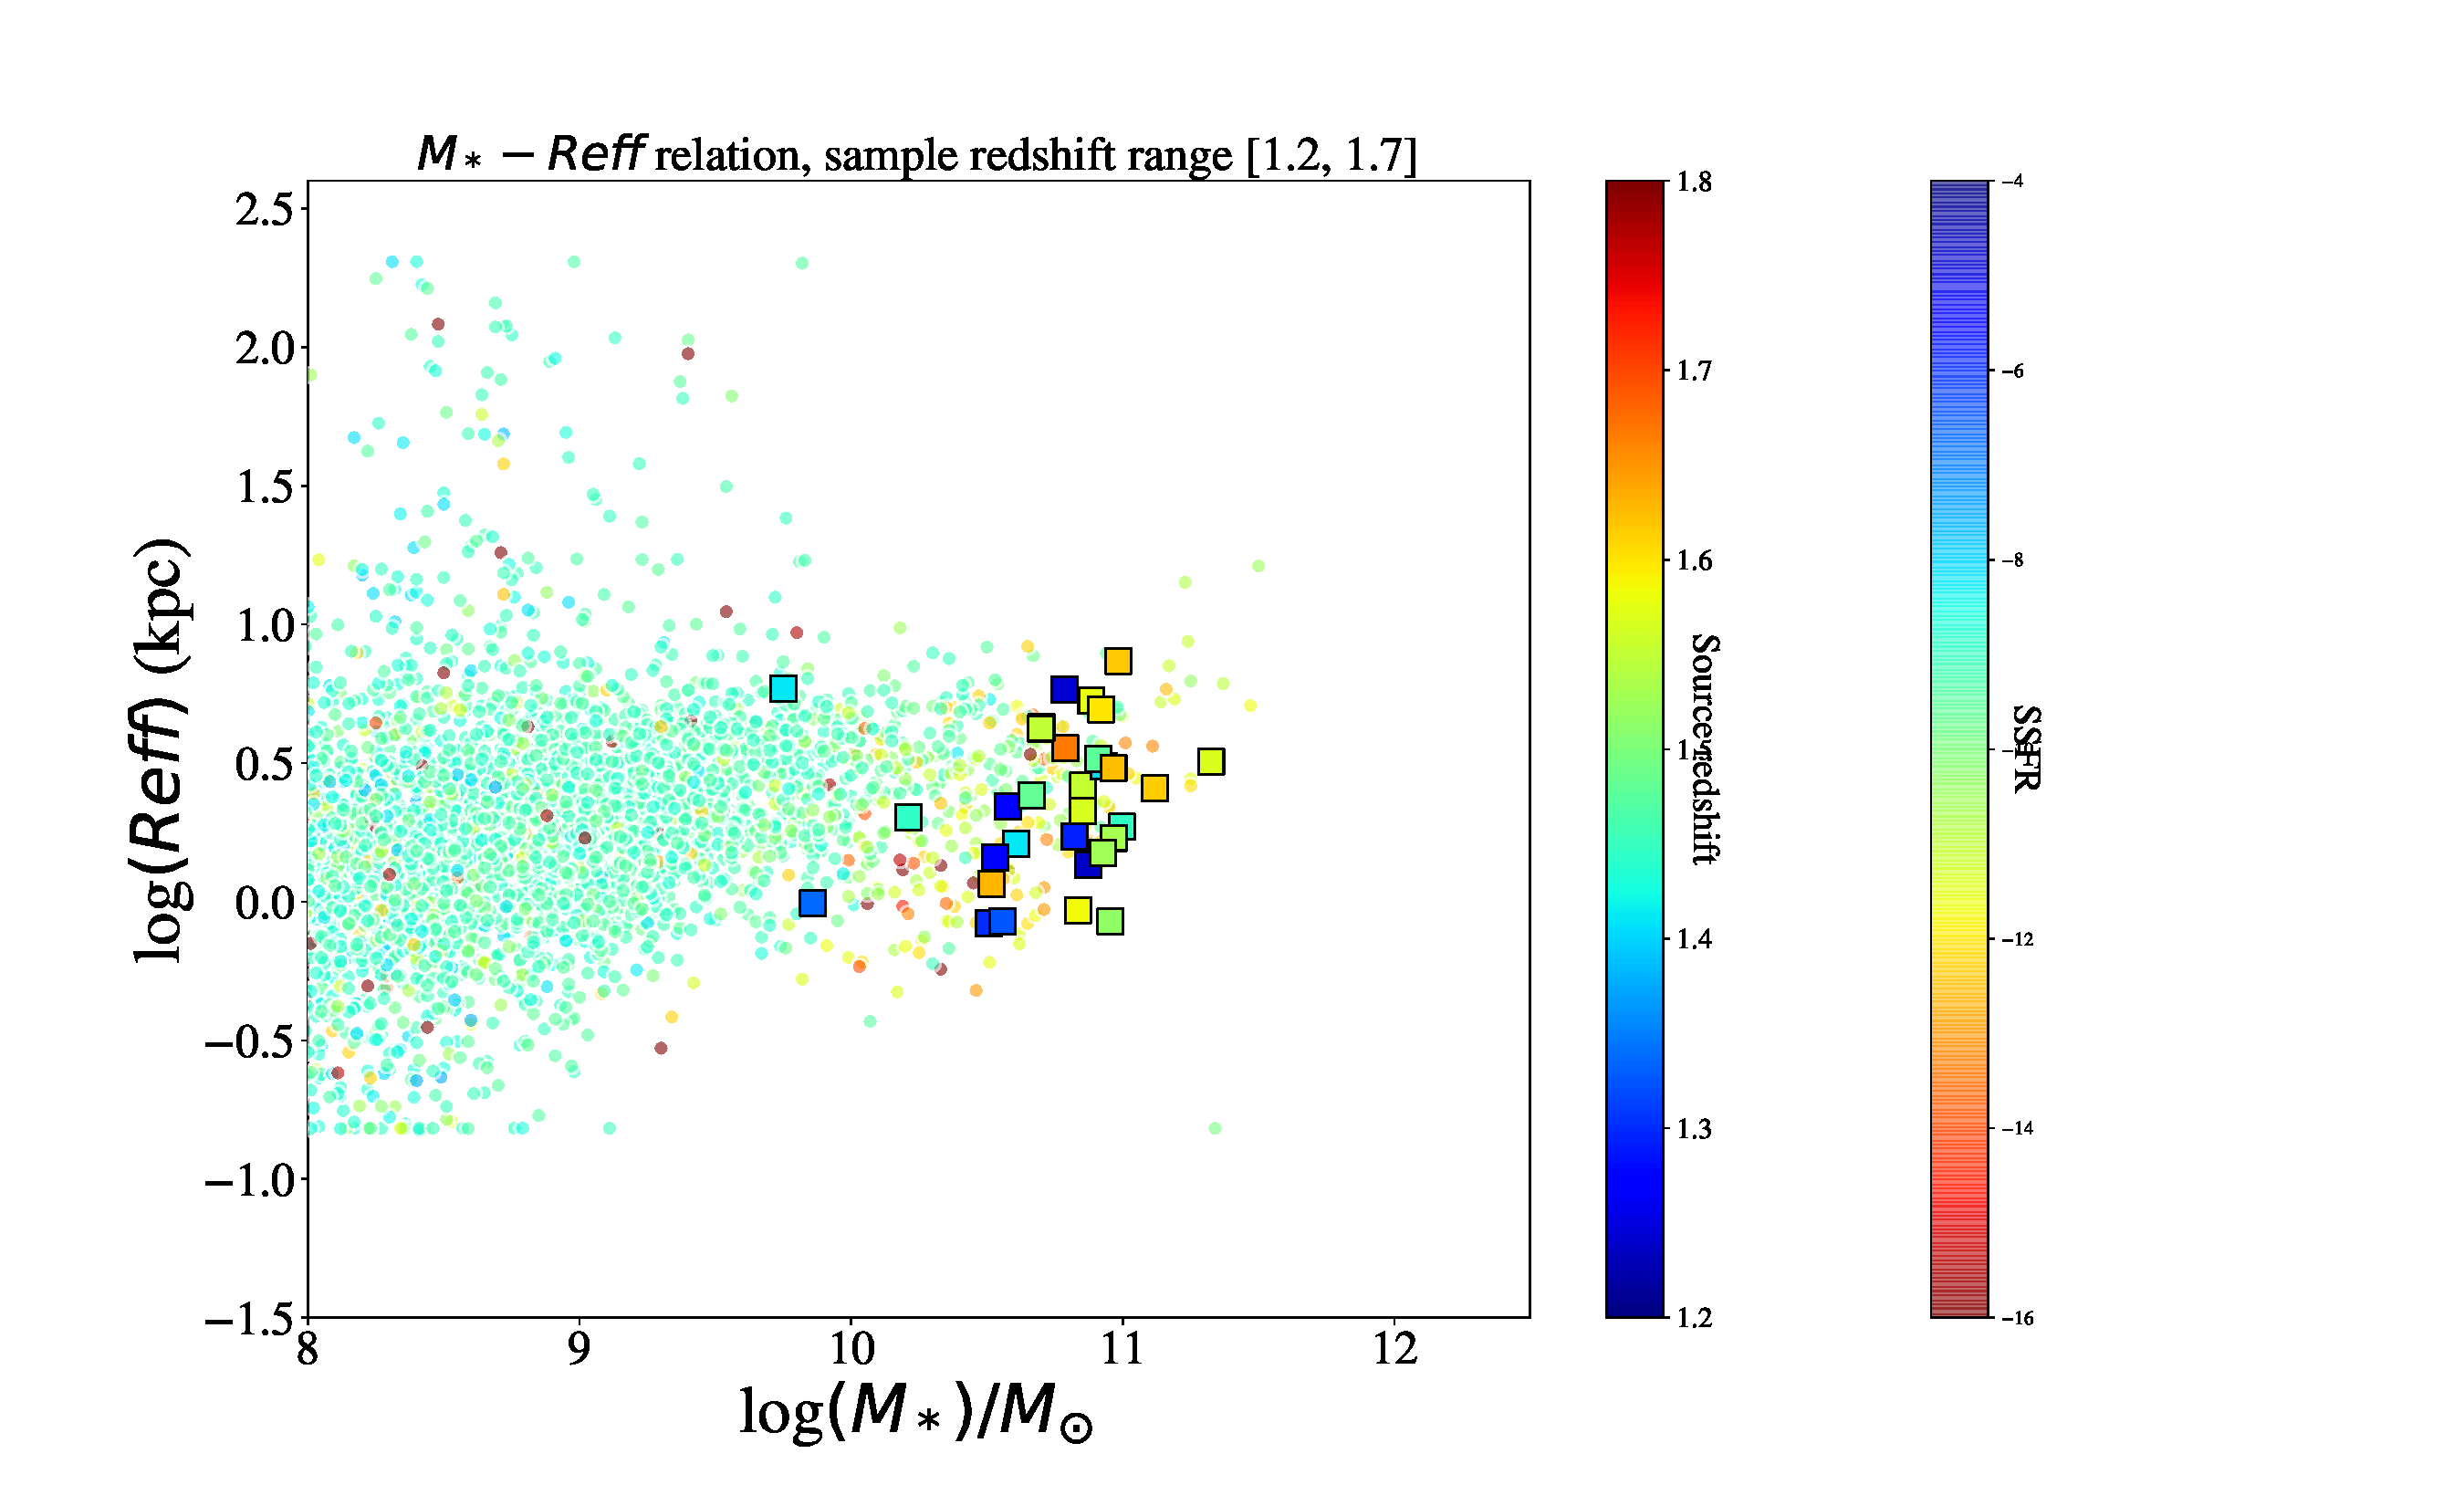
\includegraphics[trim = 0mm 0mm 90mm 0mm, clip, height=0.45\textwidth]{fig/Mstar-Reff.pdf}}&
{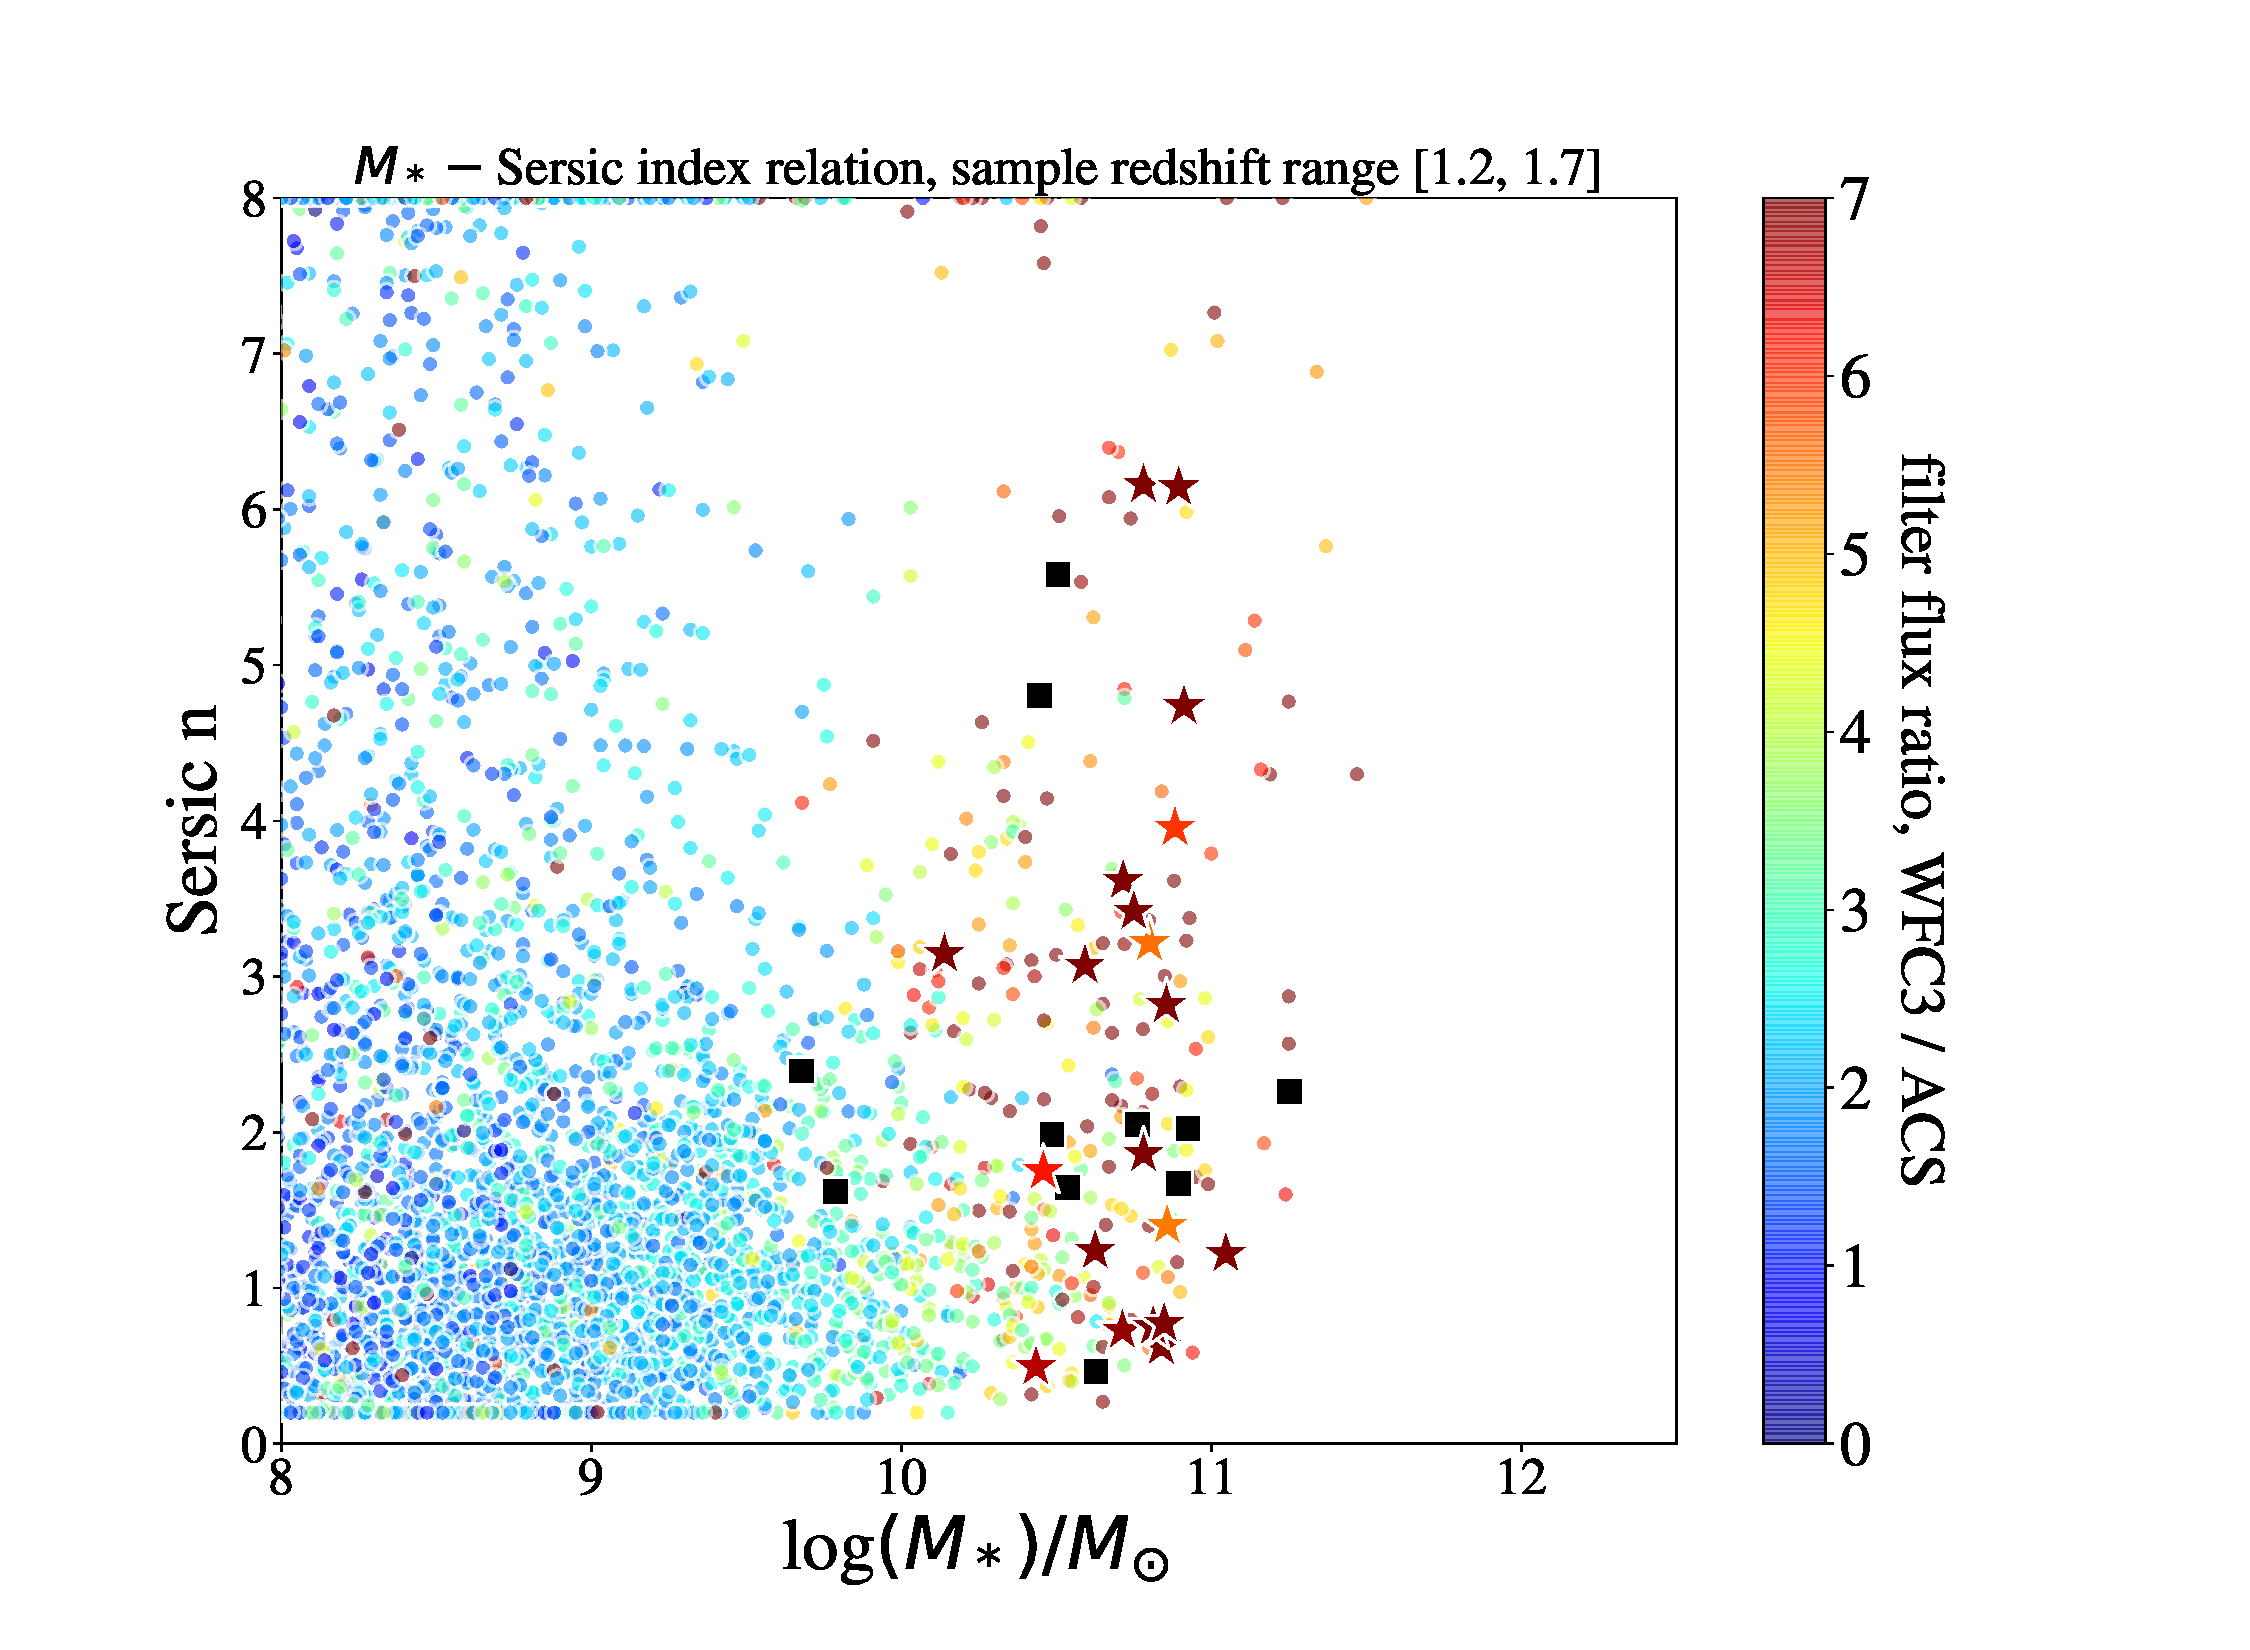
\includegraphics[ height=0.45\textwidth]{fig/Mstar-Sn.pdf}}\\
\end{tabular}
\caption{\label{fig:Mstar-rn} 
The comparison of the galaxy properties between our 32 AGNs' hosts to the 4401 CANDLES inactive sample (circles). The color coding is based on the filter flux ratio between WFC3 and ACS. For CANDLES sample, the WFC3/F125W flux is taken. The black squares are the AGN samples with only WFC3 band observation.
}
\end{figure*} 

\begin{figure*}
\centering
{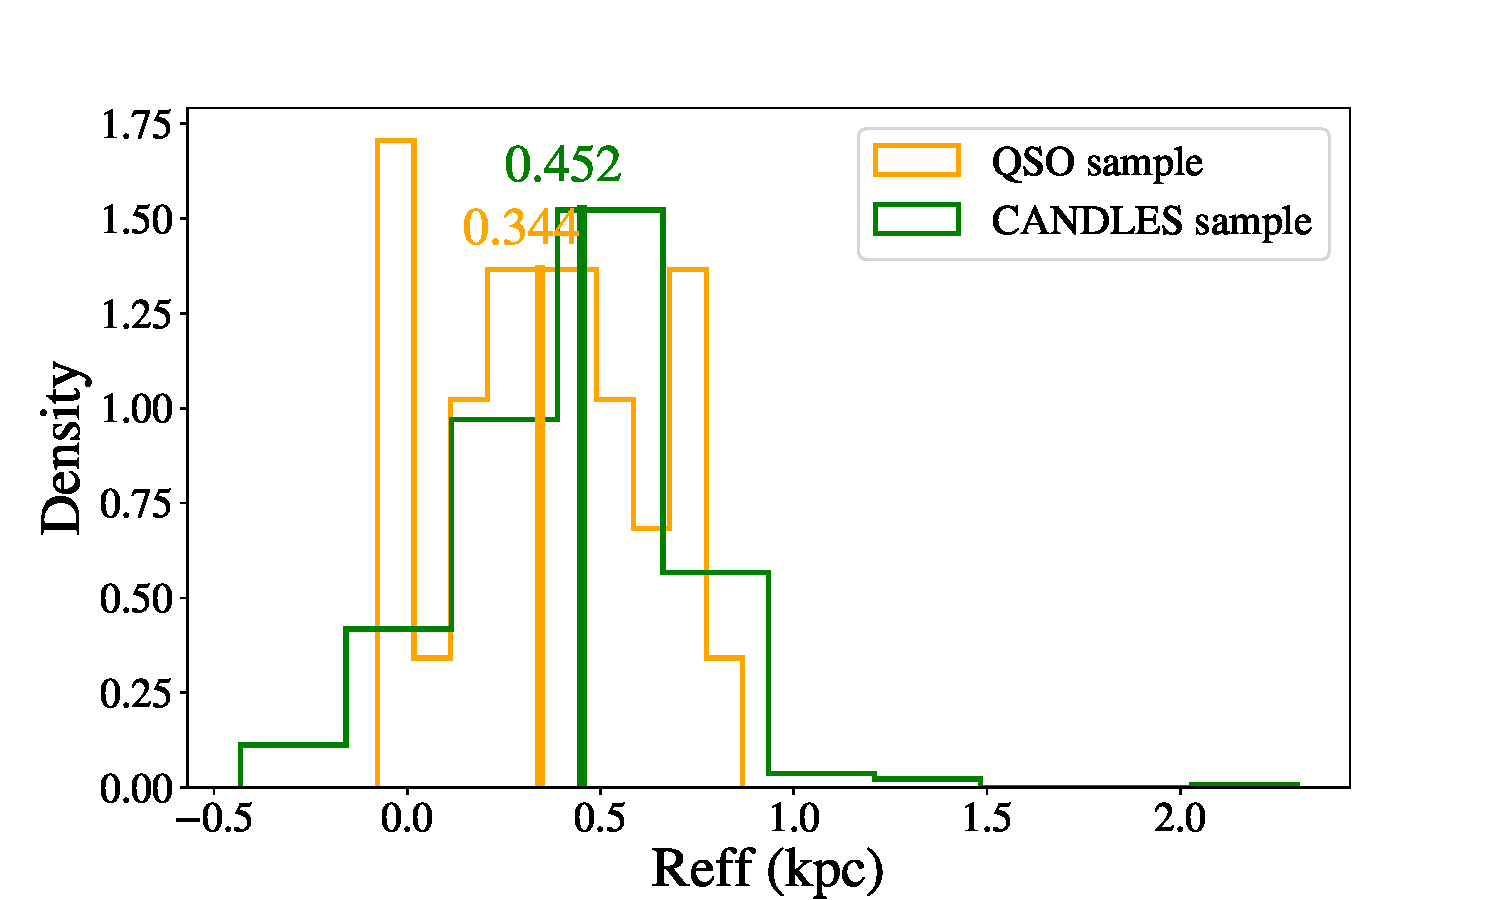
\includegraphics[ height=0.35\textwidth]{fig/Hist_Reff.pdf}}\\
{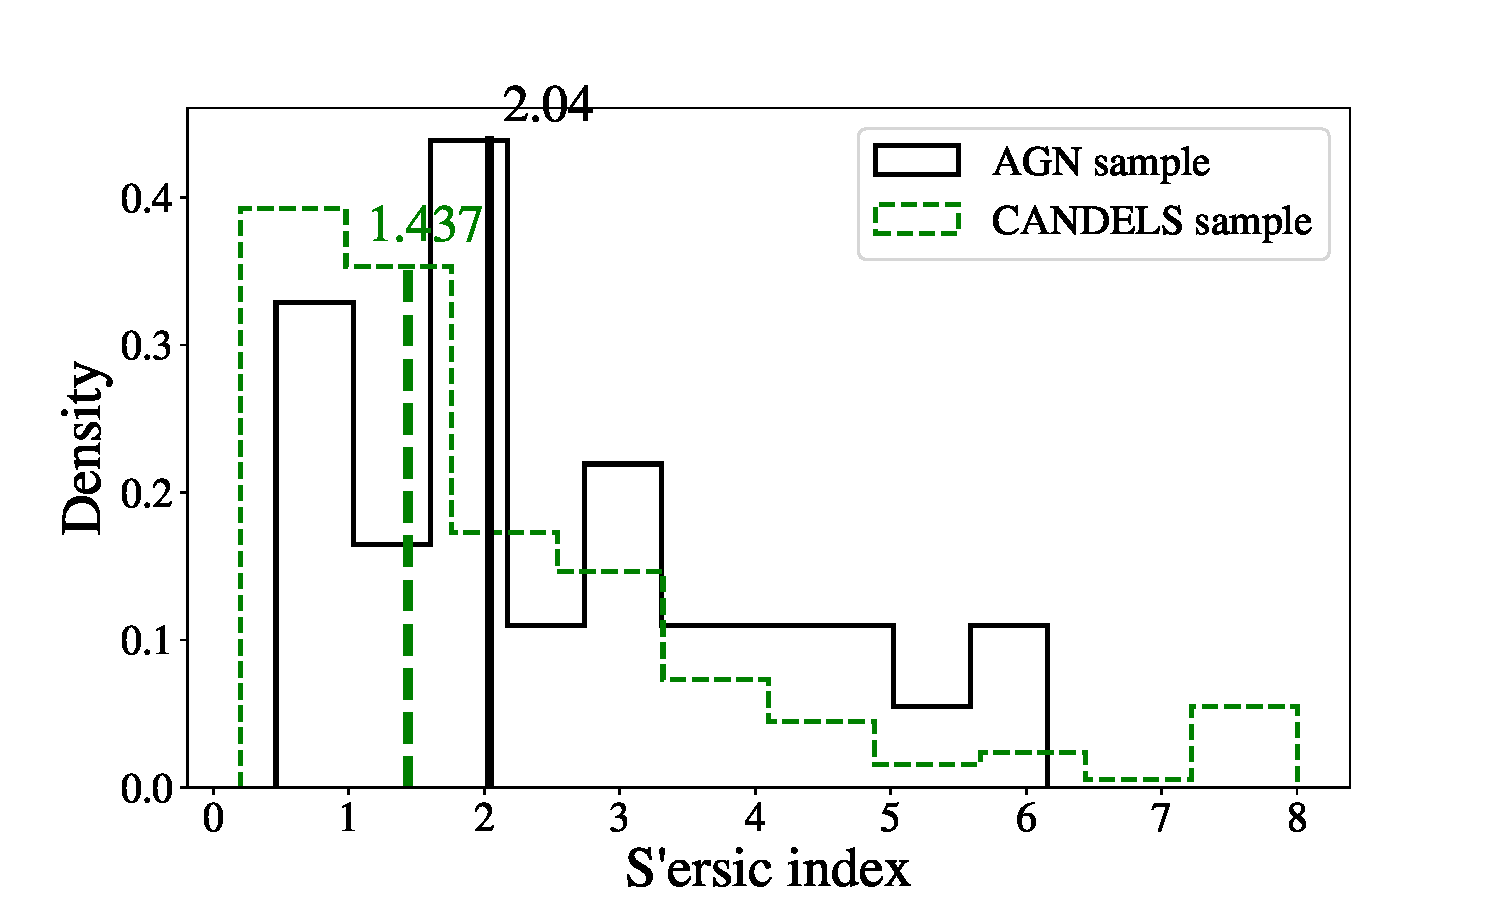
\includegraphics[ height=0.35\textwidth]{fig/Hist_Sn.pdf}}
\caption{\label{fig:hist_rn} 
The comparison of the histogram of the \Reff\ and \sersic\ n, with median value indicated.}
\end{figure*} 


%\appendix
%\section{If needed}
%\label{app:warp}

\end{document}